%------------------------------------------------------------
%                              Header
% -----------------------------------------------------------

% Document is double-sided, default font 11 points, documentclass is report
\documentclass[a4paper,11pt,twoside,final]{report}

% MY OWN SETTINGS %%%%%%%%%%%%%%%%%%%%%%%%%%%%%%%%%%%%%%%%%%%
\usepackage[utf-8]{inputenc}
\usepackage{ae,aecompl}

%palatino
% \usepackage[T1]{fontenc}
% \usepackage[sc]{mathpazo}
% \linespread{1.05}         % Palatino needs more leading (space between lines)

%day roman
%\usepackage[T1]{fontenc}
%\renewcommand*\rmdefault{dayrom}

%bera serif
%\usepackage[T1]{fontenc}
%\usepackage{bera}

%utopia (wie im neuen Tagi fuer Lauftext verwendet)
%\usepackage[T1]{fontenc}
%\usepackage{fourier}

%% Garamond Expert with NewTX Math
%\usepackage[T1]{fontenc}
%\usepackage{garamondx}
%\usepackage[garamondx,cmbraces]{newtxmath}

%\usepackage[urw-garamond]{mathdesign}
%\usepackage[T1]{fontenc}

%% times
%\usepackage{mathptmx}
%\usepackage[T1]{fontenc}

%\usepackage[Adobe Garamond]{mathdesign}

% Set section heading font
\usepackage{titlesec}
\usepackage{helvet}

\titleformat{\chapter}
  {\bf\sffamily\LARGE}
  {\thechapter}{1em}{}
\titleformat{\section}
%  {\normalfont\sffamily\Large\bfseries}
  {\normalfont\sffamily\Large}
  {\thesection}{1em}{}
\titleformat{\subsection}
%  {\normalfont\sffamily\large\bfseries}
  {\normalfont\sffamily\large}
  {\thesubsection}{1em}{}

\titleformat{\subsubsection}
%  {\normalfont\sffamily\large\bfseries}
  {\normalfont\sffamily}
  {\thesubsubsection}{1em}{}

\titleformat{\paragraph}[runin]
%  {\normalfont\normalsize\bfseries}{\theparagraph}{1em}{}
  {\normalfont\normalsize\sffamily}
  {\theparagraph}{1em}{}

\titleformat{\subparagraph}[runin] 
%  {\normalfont\normalsize\bfseries}{\thesubparagraph}{1em}{}
  {\normalfont\normalsize\sffamily}
  {\thesubparagraph}{1em}{}

\newcommand{\myparagraph}[1]{\paragraph{#1}\mbox{}\\}

\usepackage{gensymb} %provides e.g. celsius sign
\usepackage{textcomp} %provides additional signs
\usepackage{booktabs,url,array}
\usepackage[colorlinks=false]{hyperref}
\usepackage{natbib}
\usepackage{lscape}
\usepackage{multicol}
\usepackage{german}
%\usepackage[english]{babel}
\selectlanguage{english}
\usepackage{graphicx}
\setcounter{secnumdepth}{3}             % Ebenennummer, die noch nummeriert wird
\setcounter{tocdepth}{2}                % Ebenennummer, die ins Inhaltsverzeichnis 
\usepackage{pifont}                     % provides funny symbols

% Line spacing utilities
\usepackage{setspace} 

% um paper als pdf einzubauen
\usepackage{pdfpages}

% use loops to load single pdf pages
\usepackage{forloop}
\newcounter{ct}

% use package to include background image on title page
\usepackage{wallpaper}

%%%%%%%%%%%%%%%%%%%%%%%%%%%%%%%%%%%%%%%%%%%%%%%%%%%%%%%%%%%%%%%


% Use the language package german. Do not enlarge space when a new sentence starts.
%\usepackage{german}
%\frenchspacing

% Use the package dcolumn for decimal columns in tables
\usepackage{dcolumn}

% Use the package for A4 paper
\usepackage{a4wide}

% Use the AMS-LaTeX package for enhanced mathematical capabilities 
\usepackage{amsmath}

% Some more symbols (e.g., check marks)
\usepackage{amssymb}
\usepackage{pifont}
\newcommand{\cmark}{\ding{51}}%
\newcommand{\xmark}{\ding{55}}%


%-------------
% Use the fancyhdr-package and redefine headings, page numbers, etc.
%\usepackage{../sty/fancyhdr/fancyhdr}
\usepackage{fancyhdr}
% Use the pagestyle of this package
\pagestyle{fancy}
% Redefine the mark for the even side: chapternumber + chaptername in uppercase letters
%\renewcommand{\chaptermark}[1]{\markboth{\small\MakeUppercase{\thechapter.\ #1}}{}}
%\renewcommand{\chaptermark}[1]{\markboth{\small\MakeUppercase{CHAPTER \thechapter}}{}}
\renewcommand{\chaptermark}[1]{\markboth{\small\textsl{\MakeUppercase{\chaptername\ \thechapter}}}{}}
%\renewcommand{\chaptermark}[1]{\markboth{\small\textsc{\chaptername\ \thechapter}}{}}

% Redefine the mark for the odd side: sectionnumber + sectionname in uppercase letters
\renewcommand{\sectionmark}[1]{\markright{\small\textsl{\MakeUppercase{\thesection.\ #1}}}{}}
%\renewcommand{\sectionmark}[1]{\markright{\small\textsc{\thesection.\ #1}}{}}

% Clear all headings
\fancyhf{}
% Pagenumber on the left of even and on the right of odd pages
\fancyhead[LE,RO]{\thepage}
% Chapter on the right of even pages
\fancyhead[RE]{\leftmark}
% Section on the left of odd pages
\fancyhead[LO]{\rightmark}
% Draw line below heading
\renewcommand{\headrulewidth}{0.5pt}
% No footer, no line at the bottom of the page
\renewcommand{\footrulewidth}{0pt}
% Redefine pagestyle 'plain' for starting chapters: all empty
\fancypagestyle{plain}{\fancyhead{}\renewcommand{\headrulewidth}{0pt}}
% Incrase height of head a little bit
\addtolength{\headheight}{2pt}
% End of fancyhdr-Definitions
%--------------

% Use the graphicx package with the PostScript Driver dvips
%\usepackage[dvips]{graphicx}

% Redefine: minimum fraction of text on a page 
\renewcommand{\textfraction}{0.2}
% Redefine: maximum fraction of floating objects on top of page
\renewcommand{\topfraction}{0.8}
% Redefine: maximum fraction of floating objects on bottom of page
\renewcommand{\bottomfraction}{0.6}
% Redefine: minimum fraction of page that must be filled when containing only floating objects 
\renewcommand{\floatpagefraction}{0.70}

% Use the xspace package to provide a space after user defined abbreviations if one is necessary (if a word follows) and to supress the space at the end of the sentence. See the definition of \COO below.
%\usepackage{xspace}

% Define table environment modifications
\newcommand{\tophline}{\hline\noalign{\vspace{1mm}}}
\newcommand{\middlehline}{\noalign{\vspace{1mm}}\hline\noalign{\vspace{1mm}}}
\newcommand{\bottomhline}{\noalign{\vspace{1mm}}\hline}
\newcommand{\specialcell}[2][c]{%
  \begin{tabular}[#1]{@{}c@{}}#2\end{tabular}}


% Use the booktabs package to make nice lines in tables
\usepackage{sty/booktabs}

% Use the package caption2 for captions in smaller font
\usepackage[footnotesize]{caption2}
% possible options: see 'Using imported graphics in LaTeX2e, p.52
% Indent captions at each side
%\setcaptionmargin{1cm}
% Write 'Figure' and 'Table' in bold font
\renewcommand*{\captionlabelfont}{\small\bfseries}
\renewcommand\captionfont{\small\sffamily}

% Use the package flafter to make sure floating objects appear after their declaration in the text
\usepackage{flafter}

% Use the package endfloat to move all figures to the end of the text
% 
% \usepackage{endfloat}
% \nofiglist
% \notablist
% \renewcommand*{\figureplace}{%
%    \begin{center}[\figurename~\thepostfig\ etwa hier.]\end{center}}%
% \renewcommand*{\tableplace}{%
%    \begin{center}[\tablename~\theposttbl\ etwa hier.]\end{center}}%

% Enlarge line spacing (doppelter Zeilenabstand => 1.6)
% \linespread{1.6}

% Use the Journal of Geographical Research package to make the bibliography
% Note: in 'jgr_g' (german version of 'jgr') the 'and' is changed to 'und' (e.g. Stocker und Stauffer 98 instead of Stocker and Stauffer 98)
%\usepackage{../sty/jgr}

% Set indent(Einzug) = 0 at the beginning of new paragraphs
\setlength{\parindent}{0cm}

% Change the \paragraph{} style (see LaTeX Begleiter, p. 26)
% \makeatletter
% \renewcommand{\paragraph}{\@startsection
% {paragraph}% Name
% {4}% Ebene
% {0mm}%Einzug
% {0.7\baselineskip}%Vorabstand
% {-0.00mm}%Nachabstand
% {\normalfont\normalsize\bfseries}}%Stil
% \makeatother


% New user-defined commands
% =========================

% \clearemptydoublepage: start a new page on the right side of the book (odd page number).
% Used before the \chapter command and in similar cases
\newcommand*{\clearemptydoublepage}{\newpage{\pagestyle{empty}\cleardoublepage}}%

% Text aliases
\newcommand{\coo}{CO$_{\text{2}}$}
%\newcommand{\chh}{\ensuremath{\mathrm{CH}_4}}
\newcommand{\nno}{N$_{\text{2}}$O}
\newcommand{\chh}{CH$_{\text{4}}$}
\newcommand*{\kgpmmm}{kg\,m$^{{\text{-3}}}$\xspace}%
\newcommand*{\mmps}{m$^2$\,s$^{-1}$\xspace}%
\newcommand*{\mmmps}{m$^3$\,s$^{-1}$\xspace}%
\newcommand*{\mmpy}{mmJahr$^{-1}$\xspace}%
\newcommand*{\wpmm}{Wm$^{-2}$\xspace}%
\newcommand*{\wpmmpk}{Wm$^{-2}$K$^{-1}$}%
\newcommand*{\albedo}{$\alpha$}
\newcommand{\degC}{$^{\circ}$C}
\newcommand{\ud}{\,\mathrm{d}}
\newcommand{\dBC}{\ensuremath{\delta^{13}}C}
\newcommand{\dc}{\ensuremath{\Delta}C}
\newcommand{\degrees}{\ensuremath{^{\circ}}}
\newcommand{\PG}[2]{\mbox{\ensuremath{#1\;\mathrm{#2}}}}% Physikalische Groesse
\newcommand{\ooot}{O$_{\text{3}}^{\text{tropos.}}$}
\newcommand{\ooos}{O$_{\text{3}}^{\text{stratos.}}$}
\newcommand{\nox}{NO$_{\text{x}}$}
\newcommand{\nhy}{NH$_{\text{y}}$}
\newcommand{\nr}{N$_{\text{r}}$}
\newcommand{\nn}{N$_{\text{2}}$}
\newcommand{\nhhh}{NH$_{\text{3}}$}
\newcommand{\nhhhh}{NH$_{\text{4}}^+$}
\newcommand{\nooo}{NO$_{\text{3}}^-$}
\newcommand{\noo}{NO$_{\text{2}}^-$}
\newcommand{\rh}{R$_{\text{h}}$}


%-------------------------------------------------------------
%              Beginning of document
% ------------------------------------------------------------

\begin{document}

%================================ Cover page =================

%================================================= Title page ==========================================
\begin{titlepage}
\ThisLRCornerWallPaper{1.0}{fig/coverstyle_front.pdf}
\begin{center}
\mbox{}\\
{
\Huge\sf %\bfseries
{Climate Forcings and Feedbacks\\\vspace{4pt}
from the Terrestrial Biosphere}\\\vspace{10pt}
\Large{From Greenhouse-Gas Emissions\\\vspace{4pt}
to Anthropogenic Land Use Change}\\
}
%====================
\vspace*{1cm}
%====================
{\sf
\textbf{Inauguraldissertation}\\\vspace{3pt}
der Philosophisch-naturwissenschaftlichen Fakultät\\\vspace{3pt}
der Universität Bern
}\\
%=====================
\vspace{4.cm}
%=====================
{\sf
vorgelegt von\\\vspace{6pt}
{\Large \sf %\bfseries 
Benjamin Stocker}\\\vspace{4pt}
von M\"{o}hlin (AG)
}\\
%=====================
\vspace{4.5cm}
%=====================
{\sf Leiter der Arbeit:\\\vspace{4pt}
Prof. Dr. Fortunat Joos}
%=====================
\\\vspace{0.5cm}
%=====================
{\sf Abteilung für Klima- und Umweltphysik\\\vspace{4pt}
Physikalisches Institut der Universität Bern}\\

\mdseries 
\end{center}
% \end{table}
\end{titlepage}

\newpage
\clearpage
\thispagestyle{empty}
\cleardoublepage
\newpage

%================================ Title page =================

%================================================= Title page ==========================================
\begin{titlepage}
\begin{center}
\mbox{}\\
{
\Huge\sf %\bfseries
{Climate Forcings and Feedbacks\\\vspace{4pt}
from the Terrestrial Biosphere}\\\vspace{10pt}
\Large{From Greenhouse-Gas Emissions\\\vspace{4pt}
to Anthropogenic Land Use Change}\\
}
%====================
\vspace*{1cm}
%====================
{\sf
\textbf{Inauguraldissertation}\\\vspace{3pt}
der Philosophisch-naturwissenschaftlichen Fakultät\\\vspace{3pt}
der Universität Bern
}\\
%=====================
\vspace{4.cm}
%=====================
{\sf
vorgelegt von\\\vspace{6pt}
{\Large \sf %\bfseries 
Benjamin Stocker}\\\vspace{4pt}
von M\"{o}hlin (AG)
}\\
%=====================
\vspace{3cm}
%=====================
{\sf Leiter der Arbeit:\\\vspace{4pt}
Prof. Dr. Fortunat Joos}
%=====================
\\\vspace{0.5cm}
%=====================
{\sf Abteilung für Klima- und Umweltphysik\\\vspace{4pt}
Physikalisches Institut der Universität Bern}
%=====================
\\\vspace{0.5cm}
%=====================
{\sf Von der Philosophisch-naturwissenschaftlichen Fakult\"{a}t angenommen.}\\
\mdseries 
\end{center}
%=====================
\vspace{1cm}
%=====================
{\sf Bern, den 13.~Dezember 2013}
\hfill
\parbox[b]{4cm}{\sf
  Der Dekan: \\
  Prof.~Dr.~S.~Decurtins
}

\end{titlepage}

\newpage
\clearpage
\thispagestyle{empty}
\cleardoublepage
\newpage

\thispagestyle{empty}
\begin{figure}[ht!]
\begin{center}
  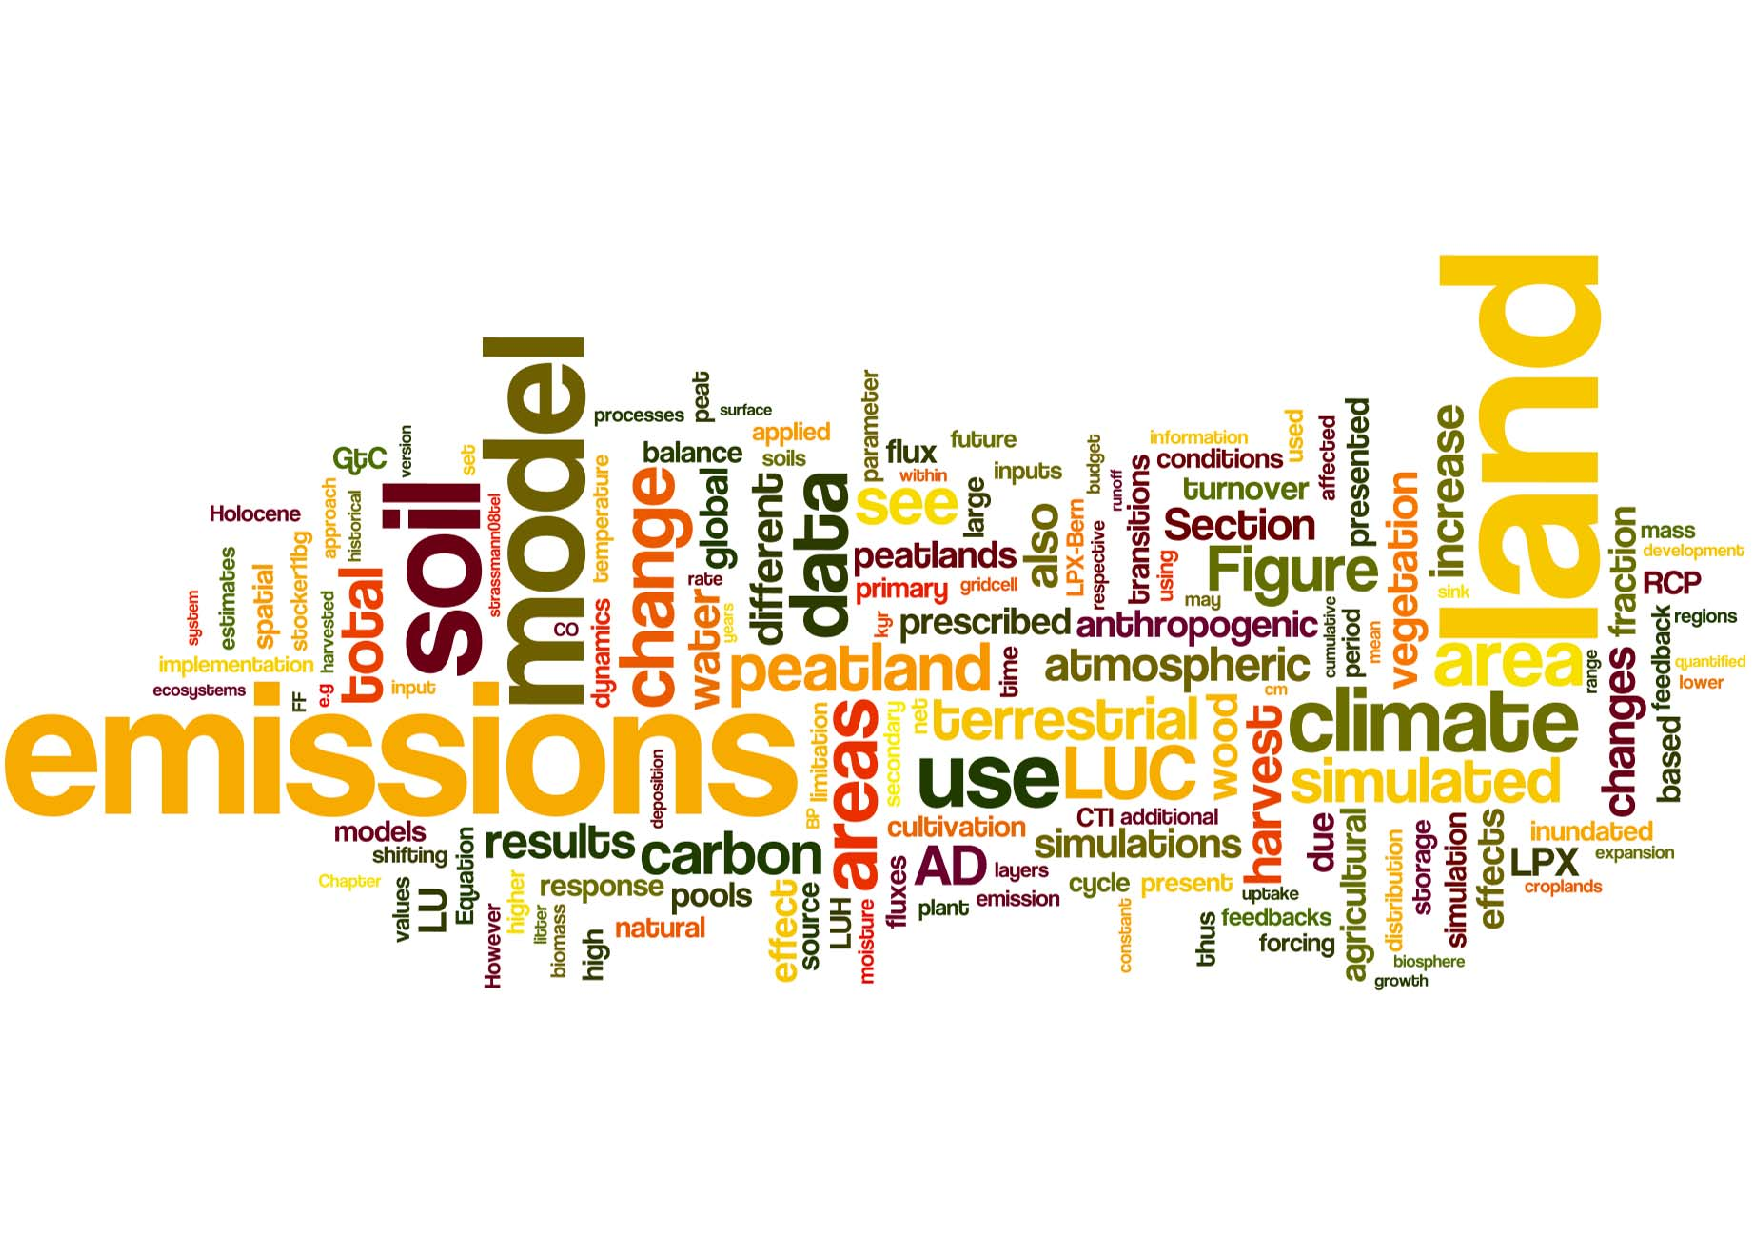
\includegraphics[width=\textwidth]{fig/wordcloud.pdf}
\end{center}
\end{figure}

%============================= Abstract ======================
\pagenumbering{Roman}
\addcontentsline{toc}{chapter}{Thesis summary}
\include{abstract}
\newpage
\thispagestyle{empty}

%============================= Table of contents  =============
\newpage
\thispagestyle{plain} \hspace{1cm}
\thispagestyle{empty}

% Make a table of contents
\clearpage
\addcontentsline{toc}{chapter}{Table of Contents}
\textsf{\tableofcontents}

\newpage
\clearpage
\thispagestyle{empty}
\cleardoublepage
\newpage

\pagenumbering{arabic}

% %===========================================================

\chapter{Introduction}
\label{sec:intro}

% In this thesis, I present results from modelling studies investigating the strength of climate feedbacks involving the terrestrial biosphere and the effect of land use change on terrestrial C storage and atmopsheric CO2. The following section shall serve as an introduction into the role of the land biosphere in the Earth system, and shall provide a conceptual framework for the quantification ...
% The main task of my work as a Ph.D. candidate was the implementation of a terrestrial N cycle model and its coupling with the C cycle, as represented in a DGVM. In the following section, I will thus put a special focus on the role of the Nitrogen cycle in modifiying land's response to climate change and will briefly discuss the implementation of N and C cycle interactions in DGVMs. 
% This intro focuses on the current state of the system and it's response to anthropogenic climate change. 
% Paleo: see chapter XXX.

% xxx footnote explaining GtC and PgC

\section{The terrestrial biosphere as an element in the Earth system}
The Earth system can be regarded as a coupled system in which its elements (atmosphere, ocean, cryosphere,  biosphere, lithosphere) are interacting on various time scales. A primary goal of Earth System research is to understand the interactions occurring on time scales that are relevant for society in the context of anthropogenic climate change. It is now established with overwhelming evidence that anthropogenic \coo\ emissions from the combustion of fossil fuels have caused a rise in atmospheric concentrations beyond levels reached over the past 800,000 years, and that this concentration increase is the dominant driver of climate change as observed over the last decades \citep{ciais13ipcc}. \\

Any prediction of climate change in the coming decades, centuries and millennia relies on an understanding of the processes that are key to the questions {\it How fast will anthropogenic \coo\ emissions accumulate in the atmosphere? What is the climate response to changes in atmospheric \coo\ and other drivers? What mechanisms does the rise in \coo\ and the change in climate set in motion and how do they feed back to climate change?}\\

This thesis focuses on the terrestrial biosphere and how it affects atmospheric \coo\ and climate change through feedbacks and in direct response to anthropogenic impacts. The land carbon cycle, nitrous oxide (\nno ) emissions from soils, methane (\chh ) emissions from peatlands and inundated soils, and a multitude of other processes \citep{arneth10ngeo} respond to a changing climate and atmospheric composition. At the same time, emissions of these greenhouse-gases, as well as direct anthropogenic impacts on terrestrial ecosystems through land use change affect climate. In this thesis, I present results from Earth system modeling studies that addressed above mentioned impacts and mechanisms and provide a quantification of their relative potency in affecting future climate change. The conceptual framework of forcings and feedbacks and the quantification formalism adopted and extended here will serve as a guide to describe and quantify the myriad interactions and feedbacks in the terrestrial biosphere. Before turning to the introduction of this framework in Section \ref{sec:concepts}, I will provide a brief introduction into the processes that shape the role of the terrestrial biosphere in the Earth system and will focus in particular on the interaction of the carbon and nitrogen cycle. 

\section{The terrestrial biosphere in equilibrium (?)}
The terrestrial biosphere being in equilibrium with climate and atmospheric \coo\ is an approximative concept often used as a description for its pre-industrial state. It is motivated by the finding that atmospheric \coo\ \citep{siegenthaler05, macfarling06grl} and climate have been remarkably stable during the pre-industrial Holocene ($\sim$11 ka BP -- $\sim$1750 AD) and that the terrestrial carbon (C) and nutrient balances and other ecosystem properties (greenhouse-gas emissions, surface energy and water exchange, see Figure \ref{fig:bonan}) adjust to perturbations and re-equilibrate on time scales of decades to millennia. These time scales are determined by vegetation dynamics and related shifts in carbon and nutrient cycling (decades to centuries), and the relatively slow turnover times of soil organic matter pools (centuries to millennia).
 
\begin{figure}[ht!]
\begin{center}
  \includegraphics[width=\textwidth]{../fig/forests_bonan.pdf}
\end{center}
  \caption[Interactions of terrestrial ecosystems with climate]{Interactions of terrestrial ecosystems (here, in particular forests) with the climate system via surface energy exchange (A), the water cycle (B), and the carbon cycle (C). Diffuse and direct solar radiation is partially reflected or absorbed, as determined by the surface albedo. Energy absorbed from shortwave and longwave radiation, in combination with water available for transpiration and evaporation determines fluxes of heat into the soil, sensible, and latent heat fluxes. Available water is determined by the soil water balance of inputs (infiltrating precipitation and snow melt) and outputs (evaporation, transpiration, surface runoff, drainage, and submilmation). Available water limits the rate of photosynthesis, which acts as the fixation of atmospheric \coo\ and provides C used for the assimilation of foliage, stem, or root biomass, exudates (not shown) or is directly respired (autotrophic respiration). Assimilated biomass turns over as litterfall, feeds the soil carbon pool, and is remineralized by microbial activity, mobilising nutrients essential for the assimilation of new tissue. Figure from \citet{bonan08}.}
\label{fig:bonan}
\end{figure}
The equilibrium concept implies that no net C fluxes occur between the terrestrial biosphere, the ocean and the atmosphere, and that all other properties remain constant. This is remarkable in the view of the vast C reservoirs on land and the large gross exchange fluxes (see Figure \ref{fig:ccycle}). Globally, $\sim$120 PgC/yr\footnote{Unless referenced otherwise, values are from \citet{ciais13ipcc} and represent present-day conditions. C fluxes and stocks are given in units of PgC$=$petagramm carbon. 1 PgC = 1 GtC = 10$^{15}$gC} are assimilated by terrestrial photosynthesis (gross primary production, GPP), and $\sim$60 PgC/yr are retained to assimilate vegetation biomass (net primary production, NPP) \citep{gruber04book}. The vegetation C stock amounts to 350 to 550 PgC and is turned over on time scales of years (grass, leaves) to centuries (stems). Turnover feeds soil C stocks (1500 to 2400 PgC), where it is retained for centuries to millennia, and is ultimately respired back to the atmosphere as \coo\ (heterotrophic respiration, \rh ). Peatland C stocks ($\sim$600 PgC, \citet{yu10grl}) have even longer lifetimes due to anaerobic soil conditions inhibiting decomposition. The turnover time (lifetime) of a given C reservoir determines its time scale of response to a perturbation. Large C stocks are contained in permafrost soils ($\sim$1700 PgC, including yedoma and deltaic deposits, \citet{tarnocai09gbc}) where C is practically locked away from the C cycle but can be re-mobilised upon thawing.\\
\begin{figure}[ht!]
\begin{center}
  \includegraphics[width=0.95\textwidth]{../fig/ccycle_ipcc.pdf}
\end{center}
  \caption[The carbon cycle]{Terrestrial and oceanic carbon cycle. Reservoirs (boxes), gross, and net exchange fluxes, and their anthropogenic perturbation given in red. Figure from \citet{ciais13ipcc}}
\label{fig:ccycle}
\end{figure}

Note that on millennial time scales, the C cycle has only very minor long-term sinks (e.g., oceanic sediment burial, peat buildup), and that any perturbation of the equilibrium induces a {\it redistribution} of C within the different reservoirs. Until equilibration, net fluxes between reservoirs occur mostly in the form of gaseous \coo . In contrast, other greenhouse-gases (e.g., \nno , \chh ) have considerable sinks in the atmosphere and, to a lesser degree, in soils. Thus, net land-to-atmosphere and ocean-to-atmosphere fluxes persist also in a C cycle equilibrium and scale atmospheric concentrations.\\

The concept of a pre-industrial land C cycle equilibrium is approximative because {\it (i)} climate and \coo\ conditions were not perfectly stable but responded to volcanic activity, changes in solar radiation, and slow changes in orbital configurations \citep{wanner08}, {\it (ii)} anthropogenic land use change has had profound impacts on local ecosystem functioning since its first appearance at the turn of the Neolithicum and caused significant global impacts on the carbon cycle and climate probably as early as $\sim$1000 BC (see Chapter \ref{sec:holoLU}), {\it (iii)} a small net C sink in peatlands has persisted even millennia after their establishment at the end of the Last Deglaciation due to the extremely slow turnover rates of soil organic matter under anaerobic conditions (see Chapter \ref{sec:topmodel}), {\it (iv)} dynamics of permafrost buildup are likely to evolve on multi-millennial time scales as well, implying long-term disequilibrium fluxes, and {\it (v)} a small burial flux of terrigenous organic matter in inland lakes and coastal zones causes a continuous sink of C (see Figure \ref{fig:ccycle}).

\section{The terrestrial response to the anthropogenic perturbation}
The pre-industrial ``equilibrium'' has been dramatically perturbed since fossil energy sources have been used and have enabled the development of industrial production and the modern lifestyle. The \coo\ emitted from the combustion of fossil fuels has accumulated in different reservoirs of the land and ocean carbon cycle (see Figure \ref{fig:ccycle}) and has wide ranging consequences for climate, ocean acidification, primary productivity of the biosphere, and the cycling of nutrients. The industrialisation has been accompanied by an increase in global population, a shift in consumption patterns and a growing demand for food. The associated expansion of agricultural land  has transformed $\sim$30\% of the land surface (\citet{hurtt06gcb}, see Chapter \ref{sec:lutrans}), while the production of mineral fertilisers, necessary to support today's agricultural production, has fundamentally disrupted the natural nutrient cycles and, e.g., amplified soil \nno\ emissions (see Chapter \ref{sec:multiGHG}). This has led to the accumulation of an array of radiatively active substances in the atmosphere and has contributed to anthropogenic climate change, eutrophication of ecosystems, loss of biodiversity, and impacts on human health \citep{ena_all}.\\
%\begin{figure}[ht!]
%\begin{center}
%  \includegraphics[width=1.1\textwidth]{../fig/rf_ipcc.pdf}
%\end{center}
%  \caption{}
%\label{fig:rf_ipcc}
%\end{figure}

The terrestrial biosphere affects the most important drivers of the radiative forcing responsible for observed anthropogenic climate change \citep{spm13ipcc}. Part of the land-mediated radiative forcings are the direct result of anthropogenic impacts on terrestrial ecosystems. For example, fertilising agricultural soils with reactive N (\nr )\footnote{\nr\ refers to all reactive mineral N species (most importantly \nhy , \nox ) and N bound in organic compounds.} causes an increase in \nno\ emissions. However, \nno\ emissions are also amplified by changes in climate and atmospheric \coo\ (see Chapter \ref{sec:multiGHG}). It is thus crucial to conceptually distinguish external forcings and feedbacks. An external forcing is defined here as a perturbation of the Earth system associated with a radiative forcing and not affected by the state of the Earth system. In the context of Earth system modeling, the ``forcing part'' of the \nno\ emission change in the example given above can be assessed when changes in climate and \coo\ (blue and red arrows in Figure \ref{fig:schematic_fb_frc}) are {\it not} communicated to the land model. In contrast, a feedback is triggered by an initial perturbation of the state (e.g., atmospheric \coo\ or climate) and feeds back to modify the ultimate response of the system to an external forcing (see also Section \ref{sec:concepts}). Following again above example, including the feedbacks requires a coupled model setup where the land module ``sees'' changes in climate and \coo . The ``feedback part'' is then captured by the difference of the coupled and un-coupled simulations. The mathematical framework of the feedback quantification is explained in Section \ref{sec:concepts}.
\begin{figure}[h]
\begin{center}
  \includegraphics[width=\textwidth]{../fig/schematic_feedback_forcing_newstyle-crop.pdf}
\end{center}
  \caption[Schematic of forcings and feedbacks related with terrestrial biosphere]{Schematic of forcings and feedbacks related with terrestrial greenhouse gas emissions and biogeophysical changes. External forcings to this system are given in yellow, and act either on the terrestrial biosphere directly (land use and land use change, LU and LUC; \nr -deposition; air pollution (\ooot, sulphate deposition, etc.) or modify the atmospheric composition (direct anthropogenic emissions). Land biogeochemical (greenhouse-gas) emissions and biogeophysical changes are affected by external forcings acting on the land, as well as by the feedback drivers (atmospheric \coo and climate). Changes induced by these drivers imply feedbacks because drivers are mediated by the Earth system response to external forcings.}
\label{fig:schematic_fb_frc}
\end{figure}

\subsection{Climate forcings from the terrestrial biosphere}
\label{sec:terrforc}
The terrestrial biosphere acts as a forcing element in direct response to anthropogenic land use (LU) and land use change (LUC), \nr -deposition, and air pollution (tropospheric ozone, \ooot ; sulphate deposition, etc.). As a consequence, land ecosystems emit radiatively active compounds and affect the surface-atmosphere energy exchange. Effects of LU and LUC on climate are manifold, but are dominated globally by changes in the carbon cycle and the surface albedo. Global modeling results for their respective total historical forcings suggest that on the global scale, the warming effect of \coo\ emissions (biogeochemical) dominates over the cooling effect of albedo (biogeophysical) changes \citep{pongratz10grl}. % Uncertainties in respective numbers for the biogeochemical effect are linked to uncertainties in cumulative LUC-related \coo\ emissions for which the reported range is between 171 and 284 PgC (\citep{stocker11bg}, see Chapter \ref{sec:holoLU}). The range of reported biogeophysical effects is -0.05 to -0.25 Wm$^{-2}$ \citep{ciais13ipcc}.
\\

The biogeochemical effect of LU and LUC is addressed in this thesis. In particular, historical \coo\ emissions since the development of early agriculture and their effect on atmospheric concentrations is assessed in Chapter \ref{sec:holoLU}. Chapter \ref{sec:lutrans} presents results from a further development of the representation of LUC, in which the area transitions between different types of land use are simulated in a global vegetation model. Estimates from this study are at the upper range of results presented in earlier studies from our group \citep{strassmann08tel, stocker11bg} due to the additional C source from effects of wood harvesting and shifting cultivation-type agriculture, effects not included before.\\

%The conversion of natural ecosystems to croplands is generally associated with a removal of natural vegetation, a disruption of the soil structure by tillage and leads to a net loss of C. The conversion to pasture impacts C stocks depending on the extent of the associated removal of natural vegetation and on the intensity of grazing. Wood harvesting removes biomass from the natural cycling of C in natural forests and causes a general reduction of C stocks. 

Different types of models have been applied to simulate the impact of LU and LUC and to quantify related global C emissions \citep{houghton12bg,baccini12,harris12,houghton12bg}. Latest estimates from the Global Carbon Project are in the range of 1.0$\pm$0.5 PgC/yr for the period 2002-2011 \citep{lequere13essd}, which is about 10\% of total anthropogenic \coo\ emissions at present. Other direct impacts of anthropogenic activities on the carbon cycle (e.g., fire suppression, peat burning) have not yet been implemented in models used for global LUC emission quantifications. \\

The climate forcing by LU and LUC is not fully captured by its effect on the terrestrial C balance and surface albedo. Deforestation by purposely set fires is associated with emissions of a range of radiatively active compounds (e.g., \chh , CO, \nox ). Furthermore, the application of mineral fertilisers and manure on agricultural land causes a large fraction of \nr\ to be lost from soils. This sets in motion a cascade of detrimental environmental effects \citep{galloway03}, many of which (e.g., \nno\ emissions) directly or indirectly affect climate \citep{erisman11}. This will be further discussed in the context of the N cycle in Section \ref{sec:ncycle}.\\

Anthropogenic LU and LUC affects climate not only through its direct effects (as a forcing), but also by modifying the land response to changes in \coo\ and climate (by modifying terrestial feedbacks). E.g., the replacement of woody vegetation with crops implies a reduction in the mean ecosystem turnover time of C and thus reduces the \coo -driven fertilisation sink. This effect can be quantified as a flux (``replaced sources/sinks flux'', see Section \ref{sec:lucdef}) and is often counted towards LUC emissions. In contrast, ``primary LUC emissions'' as reported in \citet{pongratz09}, \citet{stocker11bg}, or in \citet{strassmann08tel} as ``book-keeping flux'' exclude any feedback effects and can be regarded as a mere forcing. This conceptual difference of the quantification of LUC fluxes implies considerable differences in reported values and has caused confusion in the scientific community as discussed in recent papers \citet{pongratz13, gasserciais13}. This highlights the importance of a conceptual framework to distinguish forcings from feedbacks. While such a distinction can neatly be achieved in the context of Earth system modeling by coupling and de-coupling model components (see Section \ref{sec:concepts}), it is often impossible in reality, as ecosystems and their observable properties are inevitably affected by changes in climate and \coo .\\

Deposition of \nr\ and air pollution are listed in Figure \ref{fig:schematic_fb_frc} as an external forcing directly acting on the terrestrial biosphere, although the strength of this forcing is determined by atmospheric concentrations of \nox , and \nhy . This is because the effect of climate on atmospheric chemistry is relatively small \citep{dentener06} and thus changes in \nr\ deposition are mainly driven by anthropogenic activities (combustion of fossil fuels, industry) rather than changes in climate. The same is (approximately) valid for \ooot , sulphate, and other reactive substances. This neglects potential feedbacks, e.g., between climate and \nox\ emissions, a precursor for \ooot , mediated through the response of wildfires or the nitrogen cycle \citep{arneth10ngeo}.\\

The \nr\ forcing (atmospheric deposition and fertiliser application) induces a net climate effect that is mainly determined by the stimulation of land C storage (negative forcing) versus its amplification of \nno\ emissions (positive forcing). Amplified \nox\ emissions also affect climate by its impacts on aerosols, \ooot , and \chh\ \citep{erisman11}. A modeling study \citep{zaehle11ngeo} and meta-analyses of observational studies indicate an overall negative \citep{vangroenigen11, liugreaver09} or a small non-significant positive net effect of \nr\ on climate \citep{zaehle11ngeo} (see also Section \ref{sec:ncycle}).\\

Other direct effects on terrestrial biospheric processes are induced by air pollution. E.g., tropospheric ozone has been shown to have detrimental effects on photosynthetic tissues and plant productivity with presumably large implications for the global terrestrial C storage \citep{sitch07}; sulphate deposition can induce carbon cycle effects through soil acidification; and increased atmospheric aerosol loadings affect the photosynthetically active radiation and the fraction of direct and diffuse radiation and may thereby stimulate canopy photosynthesis \citep{mercado09}.

\begin{samepage}
\subsection{Feedbacks from the terrestrial biosphere}
\label{sec:terrfb}
Feedbacks are triggered by terrestrial biogeochemical and biogeophysical effects in response to changes in atmospheric \coo\ and changes in climate (including all its aspects affecting terrestrial ecosystems, e.g., changes in extremes or cloud cover which affects photosynthesis through modifying share of diffuse versus direct radiation \citep{mercado09}, see Figure \ref{fig:schematic_fb_frc}). The context of anthropogenic climate change since the industrial era implies large changes in atmospheric \coo . In a narrower sense as outlined in Section \ref{sec:fbmaths}, feedbacks are triggered only by the change in global mean temperature ($\Delta T$ in Equation \ref{eqn:fbpaper}). However, the uptake of anthropogenic \coo\ by land and ocean is commonly treated as a negative feedback \citep{gregory09jclim}, since increases in atmospheric \coo\ are an inherent feature and the dominant cause of anthropogenic climate change. In future climate change scenarios, the strength of this negative feedback is thus ultimately determined by the relative share of \coo\ versus non-\coo\ forcings (see Section \ref{sec:sensitivities}).\\

\citet{arneth10ngeo} provided a comprehensive overview of different feedbacks from land ecosystems and estimated rough values for their strength. \citet{ciais13ipcc} updated this compilation with different model estimates which have become available since then. According to these results, the positive feedback from permafrost thaw may have a particularly strong effect in amplifying climate change. Results presented in Section \ref{sec:multiGHG}, in line with \citet{arneth10ngeo}, suggest that climate feedbacks from the terrestrial biosphere are dominated by the negative feedback from the \coo -induced land C sink, and the positive feedback from the temperature-driven land C source. However, this assessment did not include effects of permafrost thaw and assumed a constant extent of wetlands based on present-day observations, which primarily affects the feedback from wetlands \chh\ emissions. Chapter \ref{sec:topmodel} presents the development of a model that dynamically simulates the spatial extent of wetlands and peatlands in response to variations in climate and \coo , an important mechanism for predicting the \chh\ feedback \citep{melton13}. Results presented in Section \ref{sec:multiGHG} further indicate that today, the negative land C sink feedback is dominating and that under a business-as-usual future climate change scenario, the negative total feedback will decline due to saturating sinks and decreasing radiative efficiency of \coo\ under high concentrations.\\
\end{samepage}

A strong terrestrial C sink has been observed over the past decades (1.5$\pm$1.1, 2.7$\pm$1.2 and 2.6$\pm$1.2 PgC/yr for the 1980s, 1990s, and 2000s) \citep{ciais13ipcc}. This corresponds to 25 to 35\% of total anthropogenic \coo\ emissions. These numbers are directly linked to LUC emission estimates and their uncertainty since they are commonly derived as the difference of the total terrestrial C balance and LUC emissions. However, C sink estimates are also supported by an atmospheric inversion \citep{gurneyeckels11} and by process-based models \citep{lequere13essd}. The latter study provides a thorough account of updated results and applied methodologies for the quantification of the present-day C budget. The land's role in absorbing fossil fuel \coo\ emissions and the interannual variability of this sink is impressively illustrated by Figure \ref{fig:cbudget}.\\
\begin{figure}[ht]
\begin{center}
  \includegraphics[width=0.8\textwidth]{../fig/cbudget.pdf}
\end{center}
  \caption[The anthropogenic carbon budget (1960-2012 AD)]{The anthropogenic carbon budget (1960-2012 AD, in PgC/yr). Emissions to the atmosphere are given in the upper panel. Carbon (C) accumulation in the ocean, on land, and in the atmosphere is given in the lower panel. Cumulative emissions and total accumulation is represented by the areas between curves. The total area between curves in the upper panel and curves in the lower panel is equal and corresponds to cumulative fossil fuel, land use, and ``other emissions''. Uncertainties in each term are given by the vertical bars on the left side inside the figure. Figure from \citet{lequere13essd}.}
\label{fig:cbudget}
\end{figure}

The mechanisms behind the land C sink are not well constrained. Short-term (year-to-year) variability of the atmospheric \coo\ growth rate is to a large degree determined by the interannual variability of the terrestrial sink which, in turn, has been related to ENSO \citep{raupach08}, and volcanic activity \citep{mercado09}. This relationship has been used as a constraint for global vegetation model's sensitivity of C storage to climate change \citep{cox13}, and has been interpreted as an indication that tropical forest dieback - a positive climate feedback previously suggested as a tipping element in the system \citep{lenton08} - poses less of a threat than suggested by some of the models. Using such global scale observations as an ``emergent constraint'' for models is promising since field studies are generally limited to examining small scale ecosystem processes, while the interplay between different processes and the extrapolation of findings to the global scale often remain elusive. \\

Our own results illustrate the effect of uncertainty in climate projections on the land C sink. Depending on the magnitude (global mean) and the spatial pattern of predicted climate change under a future business-as-usual scenario, the land will turn into a sizable net C source (160 PgC) or remains largely neutral with respect to C storage (see Figure 3.c, \citet{stocker13natcc}, Chapter \ref{sec:multiGHG}). A recent inter-comparison of coupled Earth system models revealed a considerable spread of results with regard to how much additional C will be sequestered in land ecosystems by the end of the 21st century \citep{arora13}. To a large degree, this uncertainty appears to be related to the land C cycle response itself. How can processes responsible for the C sink be constrained? What processes are responsible for this sink? The persistence of the negative feedback from the terrestrial C sink depends on its response to the combination of climate change and \coo\ increase and the validity of projections of the sink strength into the future rests on the process understanding determining the currently observed sink flux. Therefore ...

\subsection{Why the sink?}
\label{sec:sink}
A range of mechanisms have been discussed to explain the current land C sink. \coo\ fertilisation, relief of nitrogen limitation by increased \nr\ deposition \citep{norby98, thornton07, zaehledalmonech11, thomas10}, forest regrowth and afforestation, changes in forest management and reduced harvest rates \citep{nabuurs13}, and the lengthening of the growing season in temperature limited ecosystems probably all play a role, but their relative contribution remains debated. The sink induced by \nr -deposition has been quantified at 0.2-0.4 PgC/yr by a range of observation-based estimates and modeling studies \citep{nadelhoffer99, liugreaver09, thomas10, zaehledalmonech11}, but uncertainties remain with regard to the C:N ratio of the sink (see Section \ref{sec:ncycle}). \\

Above all, \coo\ fertilisation of photosynthesis and gross primary productivity (GPP) is the main suspect for driving the sink. Improved light use efficiency of photosynthesis under elevated \coo\ enables enhanced \coo\ fixation rates \citep{haxeltine96}, potentially leading to more C being stored in plant biomass and soil organic matter. Criticism has been raised concerning the link between changes in GPP and the change in C storage. While models commonly assume that turnover times of individual reservoirs do not depend on \coo\ and GPP, it has been suggested that subtle shifts in the tree age distribution, disturbance regimes, and tree mortality may have an overriding effect on the terrestrial C balance, compensating for the stimulation of GPP \citep{koerner09}. Such effects are not captured by Dynamic Global Vegetation Models, the main working horses in the quantification of the land carbon budget.\\

Increased water use efficiency of C3 photosynthesis and associated C3 trees' competitive advantage over C4 grasses likely contributes to the positive response of GPP under elevated \coo . In manipulative field experiments, this effect accounted for a large part of the positive NPP response; it has been suggested as the main driver of observed ``woody thickening'' and ``greening'' in water-stressed ecosystems \citep{donohue13, wigley10}, and is key to explaining the large reconstructed expansion of tropical forests over the Last Deglaciation \citep{bragg13}, when \coo\ was rising from 190 ppm to 260 ppm \citep{monnin01}. Such observational evidence from a real ecosystem responding to a large and long-term \coo\ rise appears to lend unique support for the \coo -fertilisation hypothesis.\\

Free Air \coo\ Enrichment (FACE) experiments investigate the ecosystem response under conditions that are presumably the closest equivalent to a natural ecosystem responding to rising \coo . Only few such studies have been realized to date. \citet{norby05} documented a robust initial enhancement of NPP by 23\% across a broad range of productivity. The responses diverged after several years and declined to 9\% seven years after the start of the experiment at one site \citep{norby10}, while it was sustained at another site \citep{drake11}. Declining N availability was argued to progressively limit the initial positive response \citep{norby10}. \citet{finzi07} also pointed out the crucial role of the N cycle in determining the persistence of the positive response to \coo , and showed that either increased N uptake or better N use efficiency supported the positive NPP response over several years.\\

The key importance of C and N cycle interactions has also become evident in the context of the argument about C sink projections by C4MIP models \citep{friedlingstein06}. These models have been used for carbon cycle projections as presented in the IPCC's AR4 \citep{denman07ipcc} but do not include terrestrial N cycling. \citet{hungate03} argued that such models' prediction of 350-890 PgC sequestered by 2100 AD in a  \coo -only model setup (no climate change) would have to be countered with an uptake of 7.7 to 37.5 PgN, assuming a constant C:N ratio in trees and soils. They further argued that their estimated possible range of future N supply of 1.2 to 6.1 PgN sets a hard upper limit for C sequestration and that the models' C sink predictions are therefore not plausible. This warrants a closer look at what processes determine the cycling of N in land ecosystems in the following Section. 


\section{The terrestrial nitrogen cycle}
\label{sec:ncycle}
Nitrogen (N) is an essential nutrient for the assimilation of biomass where N is required in a relatively constant ratio to C (C:N ratio), depending on the type of tissue. Furthermore, N is required in high amounts for rubisco, the enzyme responsible for \coo\ fixation. C:N ratios are around 31$\pm$7 in herbaceous biomass, 169$\pm$43 in wood, and are as low as 15-20 in humic substances in the soil \citep{esser11}. Although C:N ratios within these pools are more flexible than the rigid Redfield ratios in oceanic living organisms, they appear to vary little also under changing environmental conditions \citep{norby01}. Any increase in the size of the C pool in the terrestrial biosphere has thus to be countered with a respective uptake and immobilisation of N in organic material. However, due to low atmospheric N inputs, high energetic costs to acquire reactive N, and the continuous and (partly) unavoidable losses, N is often limiting in ecosystems.\\

An increasing terrestrial C stock requires either that N inputs have to exceed N losses, and/or a shift of C sequestration to pools with a high C:N ratio. Otherwise, the assimilation and immobilisation of additional N induces a decline in inorganic soil N and ultimately sets an upper limit to C sequestration. Will such a "progresive nitrogen limitation" (PNL) \citep{luo04} limit the C sink? And what mechanisms determine N inputs and losses?

\subsection{Nitrogen inputs}
N cycles through terrestrial ecosystems in gaseous forms (\nn , \nox , \nhhh ), dissolved in the soil solution (\nooo\, \nhhhh ), or bound in organic compounds. The atmospheric N$_2$ reservoir is practically inexhaustible but due to the high energy requirement to break its triple-bond and convert it into reactive forms, it is like the ocean's salty water to a human dying of thirst. Ecosystems have evolved mechanisms of biological N fixation (BNF) to convert N$_2$ under high energetic requirements into reactive forms, available for the assimilation of organic material. BNF is done as a symbiosis of plants (mostly leguminoses) with soil bacteria (e.g., rhizobium), in free-living soil bacteria (cyanobacteria, heterotrophs, autotrophs) \citep{vitousek02}, or by cryptogamic covers \citep{elbert12}. In the pre-industrial era, BNF was quantitatively the main pathway of N accrual by ecosystems. Today, this may still be the case only for pristine ecosystems, not affected by the increased \nr -deposition \citep{cleveland99}. Global estimates of BNF are associated with large uncertainties and have been quantified to be between 100 to 290 TgN/yr \citep{cleveland99}, with a recent ``trend'' towards the lower end (40 to 100 TgN/yr) and a ``best estimate'' of 58 TgN/yr \citep{vitousek13}. BNF is generally viewed as being resource-intensive and is limited by low levels of available energy, high levels of \nr\ in the soil, and low availability of other nutrients (phosphorous, iron, potassium, molybdenum) \citep{vitousek13}.\\

N also enters ecosystems directly in reactive forms (\nr ) through atmospheric deposition (preindustrial $\sim$30 TgN/yr) and lightnings ($\sim$5 TgN/yr) \citep{galloway04}. In the atmosphere, \nr\ has a short  lifetime (hours - days) \citep{galloway03}, and the main sink is depostion, mostly on land \citep{dentener06}. \nr\ sources to the atmosphere are \nox\ emissions from the combustion of fossil fuels, \nox , \nno , and \nhhh\ from wildfires, and \nox , NO, \nhhh\, and \nno\ from  soils. In agricultural regions, ammonium (\nhhhh ) is the dominant form of \nr\ and originates from agricultural \nhhh\ emissions. Since the invention of the Haber-Bosch process in the 1920s to convert \nn\ into ammonium, the increase in fossil fuel burning, and the widespread cultivation of N$_2$ fixing crops, the anthropogenic production of \nr\ has soared (156 TgN/yr) and now outweighs natural terrestrial BNF \citep{galloway04}. This \nr\ enters land ecosystems either directly via mineral fertilisers on croplands (today $\sim$100 TgN/yr, \citet{galloway04, zaehle11ngeo}), or indirectly via atmospheric deposition (today $\sim$65 TgN/yr, \citet{galloway04, lamarque11cc}). 

\subsection{Nitrogen losses}
\label{sec:nlosses}
N is lost from ecosystems through microbial denitrification, leaching, volatilisation, the removal of biomass by harvest, and fires. Microbial processes have evolved to gain energy by oxidizing or reducing N compounds. Volatile forms, produced by these transformations, may be lost to the atmosphere. Leaching along hydrological pathways affects dissolved organic N (DON), nitrate (\nooo ) and nitrite (\noo ) and generally increases with increasing \nr\ inputs \citep{ena}. N bound in biomass may also be removed from the system via harvest on managed lands, and fires associated with the emissions of a range of different N species (\nn , \nox , \nno , \nhhh ) \citep{ena}.\\

Gaseous N losses via microbial processes broadly scale with the size of \nr\ pools in the soil \citep{esser11}, while the loss rates are governed by soil environmental conditions. Denitrification is the main loss pathway of \nr\ and occurs under oxygen-limited, anaerobic conditions. It is governed by the availability of \nooo\ and labile C as a energy-providing substrate for the redox-process and shows a strong temperature response, partly owing to the enzymatic response but also due to increased anaerobiosis as a result of amplified heterotrophic activity under higher temperatures \citep{butterbachbahl11}. \citet{seitzinger06} suggested that 40\% of the total \nr\ input of 270 TgN/yr (natural plus anthropogenic) is lost via denitrification and that nearly half of this ocurrs in freshwater systems. However, using data on ecosystem $\delta^{15}$N, \citet{houltonbai09} estimated the total denitrification N loss to be much lower (28 TgN/yr).\\

Nitrification is the biological oxidation of \nhhhh\ or \nhhh . It affects how much \nr\ is lost due to the susceptibility of end-products (\nooo\ and \noo ) to hydrological leaching and further reduction and gaseous loss via denitrification. The fact that \nhhhh\ is preferentially taken up by plants over \nooo\ adds to that \citep{ena}. Note that the end-product of nitrification itself (\nooo ) is still in a reactive form, for which reason nitrification is usually not referred to as a \nr\ loss pathway. Nitrification occurs in well-aereated soils but is limited by low soil moisture \citep{barnard05}. Under high soil pH, loss as \nhhh\ can become important and \nhhh\ is mainly emitted from agricultural soils with high inputs of animal manure and/or urea.\\

In general, the rate of \nr\ loss in gaseous, as well as leached forms, is an indicator for ecosystem N status \citep{davidson07, ena}. Under increasing N scarcity, more \nr\ is retained and the ratio of internal recycling versus losses (in equilibrium balanced by inputs) is high. Such conditions occur, e.g., during forest stand development after abandonment of agricultural land on highly weathered tropical soils \citep{davidson07}. When \nr\ becomes increasingly available, the N cycle becomes more "leaky", or more "open", and losses increase \citep{barnard05}. The anthropogenic acceleration of N cycling by the dramatic increase in ecosystem \nr\ inputs induces a more leaky N cycle and amplifies \nr\ losses.\\

\citet{galloway03} have documented how every molecule of \nr\ lost can cause a range of detrimental environmental effects as it is transformed within and transported between different landscape elements. The critical step is the initial formation of \nr . In the atmosphere, \nox\ and \nhhh\ contribute to aerosol formation and tropospheric ozone. \nno\ acts as a greenhouse-gas and depletes stratospheric ozone. An increasing amount of \nr\ is transferred to the hydrosphere (wetlands, rivers, estuaries), causes eutrophication and acidification and is converted back to N$_2$ by denitrification with a fraction lost as \nno\ to the atmosphere. This N cascade thus has consequences for biodiversity, human health and climate.  

\subsection{Carbon and Nitrogen cycle interactions determine N availability and uptake}
\label{sec:cncoupling}
A plant's demand for N is driven by the growth in different stores with their respective C:N ratios and is limited by the availability of N. While the ecosystem N balance is governed by inputs and losses, a plant's actual N availability under natural conditions is to a large degree determined by the decomposition (and mineralisation) rate of litter and soil organic matter. While the "classic" N cycle paradigm centers on the mineralisation rate as the bottleneck-process governing N limitation, more recent research has documented the uptake of organic N (monomers and amino acids) \citep{nasholm98,schimel04,nasholm09} and views N uptake in the light of a plant's resource economics \citep{fisher10, phillips13}. This view suggests, that under increasingly N limited conditions, a plant's allocation of C dynamically adjusts to improve its access to N (and other nutrients). 
%N uptake is thus a process associated with a cost of fixed C, while the price of N depends on the degree of N scarcity.
\\

Indeed, allocation to root growth has been documented to increase under elevated \coo\ and N limitation \citep{pregitzer08, iversen12, vangroenigen11}. Contrarily, fine root mass decreased in a warming experiment, where increased soil turnover improved N availability \citep{melillo11}. Access to N not only depends on root mass and the soil exploration by fine roots, but also on the efficiency of mycorrhizal fungi in providing mineral N to the plant. Mycorrhiza live in association with the plant and have a more efficient access to mineral N (arbuscular mycorrhiza) than roots alone and can even access organic N (ectomycorrhiza). They satisfy their energetic demands from labile C exuded by the roots \citep{phillips13}. Thereby, fungal, as well as microbial activity, fuelled by readily available energy from exuded labile C, induces a "priming effect" of (otherwise recalcitrant) soil organic matter \citep{fontaine07, cheng13, drake11}. This not only mobilises N but also affects the soil C balance.\\

Also \nn\ fixation has been suggested as a costly facultative plant strategy, deployed under N-scarce conditions, but omitted when N is abundant \citep{hedin09, barron11}. The same principle applies on the ecosystem level, where plants capable of fixing N have a competitive advantage under strong N limitation but are outcompeted when N is abundant. This dynamic adjustment of processes responsible for overcoming ecosystem N deficiency and making N available for plant uptake has been documented for forest stand development in tropical ecosystems after disturbance \citep{davidson07, yang11, batterman13}. Whether these mechanisms may prevent a "progressive N limitation" under rising \coo\ and relieve the observed N shortage after the initial NPP stimulation in FACE experiments remains to be shown.\\

While the effect of C-N interactions on the terrestrial response to \coo\ is unclear, the response to warming appears more robust. Accelerated decomposition mobilizes N \citep{bai13} and alleviates N limitation in temperate and boreal ecosystems. In a soil warming experiment, this led to an initial negative soil C balance, compensated later by a stimulation of plant growth due to the release of additional inorganic N from soil organic matter decomposition \citep{melillo11}.\\

Atmospheric deposition of reactive N generally attenuates N shortage, induces a reduction of plants' investments into N uptake and frees resources to invest into the access to other limiting factors (e.g., light). This has a positive effect on C sequestration \citep{magnani07, thomas10}. Trees with arbuscular mycorrhizal associations have been shown to benefit most from increased inorganic N pools under elevated \nr\ deposition \citep{thomas10}. But how much additional C is stored for each N added? \citet{magnani07} suggested a large \nr -deposition driven C sink with seemingly no detrimental effect under even the highest observed deposition rates. Their calculation implied a C:N ratio of 470 for this sink. A high value, that was later critisized and corrected downwards. Accounting for bulk (including dry) \nr\ deposition alone would decrease the value by \citet{magnani07} to 175 \citep{devries08}. Regarding the C:N ratios of plant pools and assumptions on allocation patterns of sequestered C reduces the ratio further to 30-70\citep{devries08, sutton08, thomas10}. Plot-level $^{15}$N tracer experiments show that most N is retained in soils, where C:N ratios are even lower \citep{nadelhoffer99, liugreaver09}. The strong positive effect of \nr\ deposition on C sequestration suggested by \citet{magnani07} has also been critisized due to their neglection of a possible upper limit \citep{deschrijver08}. Ecosystem N oversaturation under continuous high \nr\ inputs increases \nooo\ leaching and can thereby lead to soil acidification with detrimental effects on plant growth and may turn ecosystems into a source of C \citep{ena}.\\

The N cycle differs markedly between natural and agricultural ecosystems \citep{ena, butterbachbahl11}. N cycling on agricultural land is governed by fertilizer N inputs and harvest N removal, while on non-agricultural land, it is determined by the subtle balance of inputs by \nr -deposition and BNF and the losses. The pools of inorganic N is increased on managed land by the application of fertilisers and on non-agricultural land by \nr -deposition. This over-supply negatively affects N retention processes and induces an amplification of N losses and associated \nno\ emissions (see Section \ref{sec:n2o}). E.g., \citet{barton99} showed that denitrification rates are one order of magnitude higher on agricultural land than in forests. While climate and \coo\ are inducing gradual changes in the cycling and the stocks of N in terrestrial ecosystems, direct anthropogenic impacts thus have an overriding effect via controlling ecosystem inputs of \nr\ \citep{butterbachbahl11}. 

\subsection{Nitrogen limitation controls \nno\ emissions from soils}
\label{sec:n2o}
Atmospheric \nno\ concentrations have increased from $\sim$270 to $\sim$320 ppb since pre-industrial times \citep{meure06} and now contribute about 7.4\% to the total anthropogenic radiative forcing \citep{ciais13ipcc}. \nno\ has an atmospheric lifetime of about 122 years and has its sink in the troposphere where it also contributes to ozone depletion \citep{hirsch06gbc}. Today, the relative share of terrestrial to total (including oceanic) \nno\ emissions is roughly 64-74\% \citep{hirsch06gbc}. Atmospheric inversions cannot constrain this split more precisely and suggest global emissions of 14.1-17.8 TgN/yr\footnote{Numbers reported here refer to the mass of \nno -N.} \citep{huang08}, in line with a top-down estimate of 15.7$\pm$1.1 TgN/yr \citep{prather12}. Bottom-up estimates have a much higher uncertainty  (8.1-30.7) TgN/yr with a ``best'' estimate of 17.9 TgN/yr \citep{ciais13ipcc}.\\

Over Glacial-Interglacial cycles, as well as with millennial-scale climate variability (Dansgaard-Oeschger events), atmospheric \nno\ varied between $\sim$220 and $\sim$280 ppb \citep{schilt10qsr}. While \citet{schmittnergalbraith08nat} suggested that the \nno\ changes related to millennial-scale climate variability during the last Glacial (Dansgaard-Oeschger events) can be fully explained by oceanic source changes, land modeling studies found a considerable positive feedback between terrestrial \nno\ emissions and climate \citep{xuri12nphyt, stocker13natcc} (see also Chapter \ref{sec:multiGHG}), which likely contributed to the variations of atmospheric concentrations on these time scales.\\

Land sources of \nno\ are denitrification and nitrification by bacteria, archaea, and fungi in soils. Along the nitrification pathway, where \nhhh\ is oxidized to \nooo , \nno\ is produced as a by-product. Under denitrification, \nooo\ is sequentially reduced to \noo , NO, \nno , and N$_2$, the latter being most reduced form. The ratio of volatile losses of \nn\ versus \nno\ depends on the soil oxygen status \citep{simek02}. In the reduction of \nooo , denitrifying bacteria rely on labile C as a source of energy. Given the control of N limitation on root exudation of labile C, this represents a possible negative feedback on N shortage.\\

Under natural conditions, soil \nno\ emissions are often reported to be driven by high soil temperatures and to peak at soil moisture levels of around 70\% water-filled pore space \citep{davidson91, schilt10qsr}. This has been interpreted that \nno\ emissions ``essentially depend on precipitation and temperature and are therefore closely linked to climatic changes'' \citep{fluckiger04}. However, apart from the variable ratio of N lost as \nno\ versus \nn , \nno\ emissions are primarily governed by the amount of N denitrified and nitrified, thus ultimately by the size of the inorganic N pools. Soil moisture and temperature exert a control solely by modifying the nitrification/denitrification {\it rates}, while oxygen availability determines the loss pathway (denitrification versus nitrification). The size of the inorganic N pool can be viewed as a measure for N limitation. Under N scarcity, inorganic N availability decreases and N tends to be retained within the system, rather than being lost. Hence, \nno\ emissions decrease with increasing N limitation and vice versa \citep{davidson07}.\\

How does climatic change affect N limitation? The decomposition of soil organic matter (SOM) is generally accelerated under warmer soil temperatures \citep{knorr05}. In a N-limited temperate ecosystem, a soil warming experiment found that the faster SOM decomposition alleviates N limitation by releasing more inorganic N and results in an enhanced above-ground tree growth after 7 years \citep{melillo11}. However, the effect on N losses and \nno\ emissions were not reported and ultimately depend on the subtle balance between changes in decomposition and N mobilisation rates and changes in N demand and uptake by stimulated growth. Meta-analyses found that elevated \coo\ had a positive, or no significant effect on \nno\ emissions, and relatively large uncertainties remain \citep{vangroenigen11}.\\ 

% ena (varying deposition effects {on what?} interpreted as initial N status)

In agricultural soils and in ecosystems affected by enhanced anthropogenic \nr\ inputs, N limitation is relieved and \nno\ emissions increased \citep{barnard05}. This direct anthropogenic impact has an over-riding effect on \nno\ emissions, dominating the more subtle responses to changes in climate and \coo\ under natural conditions \citep{barnard05, butterbachbahl11}. The fraction of \nr\ added that is lost as \nno\ is commonly referred to as the \nno\ emission factor and quantified at 1\% \citep{IPCC2006} to 5\% \citep{crutzen08atmchemphys,davidson09natgeo}. Our own results presented in Section \ref{sec:multiGHG} suggest that the effect of climate and \coo\ in controlling \nno\ emissions from agricultural soils are substantial and might amplify this \nno\ emission factor in a high-warming scenario. Thus, terrestrial \nno\ emissions as a ``climate feedback element'' might gain in importance relative to terrestrial \nno\ emissions being primarily a ``climate forcing'' controlled solely by anthropogenic \nr\ inputs. 

\section{N cycle representations in global vegetation models}
\label{sec:nmodels}
A range of global vegetation models simulating the coupled cycling of carbon and nitrogen have been presented since the multi-model carbon cycle projections in the IPCC AR4 \citep{denman07ipcc}. These models differ with respect to the implementation of particular N cycle processes, as well as in their focus on which processes are resolved in what detail. No concerted model inter-comparison of this generation of models has been conducted to date. However, \citep{zaehledalmonech11} provide a thorough account of available models and their individual implementations. Here, I will briefly touch upon some of the features which, in my view, are key to generating long term N limitation and determining the long-term C sink. Section \ref{sec:dyn} then provides a brief description of the N cycle implementation in DyN-LPJ, the ``template'' for LPX-Bern, the model applied for the studies presented in this thesis.\\

As discussed in Section \ref{sec:cncoupling}, the long-term effect of C-N coupling on terrestrial C sequestration is primarily controlled by the balance of N losses and inputs and whether N can be retained under N limitation or whether more N can be made accessible either through upscaling BNF or mining additional SOM to satisfy the increasing demand. On the input side, some models \citep{zaehle10ocn1, jain09} formulate BNF as being constant based on climatic variables. This is likely to lead to conditions of progressive N limitation. On the other extreme, BNF scales with plant productivity and should thus tend to satisfy an increasing demand \citep{xuri08gcb, thornton07}. Resource limitation on the capacity of plants to acquire N through BNF, a concept with strong observational support (see Section \ref{sec:cncoupling}), is treated only by few models \citep{fisher10, esser11, gerber10}. Interestingly, one such model suggests no long-term N deficiencies under elevated \coo\ with 8.5 PgN additional BNF \citep{esser11}. This is beyond the upper limit of total additional N inputs suggested by \citep{hungate03}. Explicit interactions with the rhizosphere through labile C exudation and energy limitation of SOM decomposition is not implemented in any global model.\\

On the loss side, simple representations are based on a hole-in-the-pipe approach, where a constant fraction of mineralized N is lost \citep{gerber10, wang10}. This implies that N losses are independent of N limitation and the size of inorganic N pools. Thus, no N retention mechanism is at play, unless N is retranslocated within the plant before leaf abscission \citep{fisher10}. More sophisticated parametrisations of nitrification and denitrification explicitly treat a varying inorganic N pool \citep{thornton07} and few \citep{zaehle10ocn1, xuri08gcb} have adopted simplified versions of complex site-scale models (DNDC-type, \citet{li00}) where nitrification, denitrification, leaching, and volatilisation are simulated with an explicit treatment of the most relevant substrate pools (\nooo , \noo , NO, \nhhh , labile C). These models are also able to capture effects on \nno\ emissions assuming constant ratios of N lost as \nno\ versus \nn . To date, only O-CN \citep{zaehle10ocn1} and LPX-Bern \citep{stocker13natcc} have been applied to simulate the dynamics of C and N cycling, effects on \nno\ emissions, and their feedback with climate and the carbon cycle. \\

Observational evidence for flexible C:N stoichiometry is somewhat inconclusive \citep{norby01, finzi07, norby05}, potentially causing considerable uncertainty in C sink projections. Most models assume a constant C:N ratio in individual plant pools, and few allow for flexibility within constraints \citep{xuri08gcb}, restricted elasticity \citep{zaehle10ocn1}, or by the buffering of short-term fluctuations in N availability by a temporary storage pool \citep{gerber10}. However, small changes in C:N ratio over the 21st century are predicted by one model which allows for flexibility \citep{esser11}.\\

Key results of this generation of global vegetation models are that (i) the positive response of terrestrial C storage to \coo\ is reduced, and that (ii) land C losses caused by warmer temperatures are attenuated. The latter effect is found in all models and is due to the additional N released by enhanced SOM decomposition, an effect robustly backed by observational studies \citep{melillo11}. C-N effects on the response to \coo\ show a large spread, probably due to the models' different implementations of mechanisms determining N limitation. The C sequestration by 2100 AD is reduced by effects of C-N interactions by 31\% in O-CN \citep{zaehle13}, by 74\% in CLM-CN \citep{thornton07} and by less than 10\% in LPX-Bern. 

\section{N cycle representation in DyN-LPJ}
\label{sec:dyn}
The DyN-LPJ (Dynamical Nitrogen cycle-LPJ) by \citet{xuri08gcb} has been adopted in LPX-Bern to capture C-N coupling effects, soil inorganic N dynamics and associated \nno\ emissions. This is a further development of the Lund-Potsdam-Jena Dynamic Global Vegetation Model LPJ-DGVM \citep{sitch03gcb}. Dynamic Global Vegetation Models (DGVMs) represent not only terrestrial C (and N) cycling but also the vegetation dynamics based on plant functional types (PFTs) in response to climate. A full account of the equations and parameter values implemented in DyN-LPJ is provided in the original publication \citep{xuri08gcb}. Figure \ref{fig:dyn} serves as a graphical illustration and represents the most important flows, stocks, and transformation processes of N in DyN-LPJ. A documentation of the adoption of DyN-LPJ into LPX-Bern and the necessary modifications is provided in Appendix \ref{sec:app.lpx}. This version of LPX-Bern (version 1.0) has been used in \citet{stocker13natcc} to quantify different feedbacks between land and climate (see Chapter \ref{sec:multiGHG}).\\ 
 
Dynamics of soil inorganic N are resolved in DyN-LPJ with relatively high process detail following a scheme of DNDC-type (\citet{li00}, see Section \ref{sec:nmodels}). On the other hand, its C-N coupling can be loosely described as ``weak''. E.g., inputs of N (a surrogate for all types of BNF) indirectly scale with plant productivity, as the soil C:N ratio is held constant and an implicit N influx is governed by the soil C inputs from litter decomposition  (see Figure \ref{fig:dyn}). Although on the short term, N limitation can occur as N uptake is limited by the availability of inorganic N, the system tends to bring in additional N on the long-term when productivity is enhanced (e.g., under elevated \coo ). In DyN-LPJ, soil temperature and soil moisture govern N availability which can induce N limitation under cold temperatures. Compared to the C-only model setup (in LPX-Bern), this leads to significantly reduced productivity and C stocks at high northern latitudes and required some adjustments to bring soil stocks back to better agreement with observations (see Appendix \ref{sec:app.lpx}).\\

\begin{figure}[ht!]
\begin{center}
  \includegraphics[width=\textwidth]{../fig/DyN_schematic_newstyle.pdf}
\end{center}
  \caption[Simplified schematic of the N cycle in DyN-LPJ]{Simplified schematic of the N cycle in DyN-LPJ. Flow of organic N mass is given in blue arrows, stocks are represented by rectangles. Inorganic N dynamics are in red. C flows and stocks are in green. Important information flow is given by dashed arrows. N uptake is driven by the N demand and limited by the availability of inorganic N (\nhhhh , \nooo ), temperature, and soil moisture (not shown). The N demand is determined by NPP and the constant C:N ratio of new tissue. NPP is downscaled so that the demand is met by the availability. C allocation to leaves, sapwood, and roots is not affected by N availability, while N is allocated according to constant relative C:N ratios in leaves vs. sapwood, and leaves vs. roots. Litterfall determines the C:N ratio in litter, and a constant fraction of litter turnover enters the soil pool, the remainder C is respired (R$_{\text{h}}$) and N mineralised to \nhhhh . The soil organic N stock is determined based on a constant prescribed soil C:N ratio and the soil organic C stock, which receives inputs from litter decomposition. As soil C:N ratios are generally smaller than those of litter decomposition, this implies an additional N input to the system, indicated by the '?'. SOM mineralisation feeds the \nhhhh\ pool, where it is subject to volatilisation as \nhhh , or nitrification to \nooo\ with associated \nno\ emissions. The fraction of leached \nooo\ is determined by surface plus drainage runoff as a fraction of total soil water content. Denitrification rates depend on temperature (like nitrification), as well as on labile C availability, here given by the daily litter decomposition. The partinitioning of substrate pools subject to nitrification versus denitrification is determined by soil moisture, assuming that both processes occur in parallel in aerobic and anaerobic microsites. Complete equations and parameter values are given in \citet{xuri08gcb}.}
\label{fig:dyn}
\end{figure}

Generally put, N limits C sequestration in DyN-LPJ on the short-term, and predominantly via temperature. Elevated \coo\ stimulates NPP and ultimately the turnover of litter and SOM. This releases more \nr\ and amplifies \nno\ emissions. The effect of \nr -deposition is weak for C sequestration as the model tends not to be N limited. Thus, \nr\ additions primarily increase the inorganic N pools with direct effects on N losses and \nno\ emissions. These model characteristics are reflected in published results \citep{xuri12nphyt, stocker13natcc} and in Figure \ref{fig:betagamma}, Section \ref{sec:multiGHG}. \\

DyN-LPJ and LPX-Bern results can be compared to the results of the O-CN model presented in \citet{zaehle11ngeo}. 
%Do date, the O-CN model is the only other coupled global carbon cycle-climate model that has been applied to investigate effects of anthropogenic \nr\ inputs on C sequestration and \nno\ emissions. 
In their study, \nr\ addition induces an additional cumulative C sink of 12 PgC, or 0.2 PgC/yr for the period 1996-2005 AD. In LPX-Bern, this effect is almost negligibly small (see Figure \ref{fig:betagamma}). Respective observational studies tend to support the findings by \citet{zaehle11ngeo}. On the other hand, O-CN simulates small effects of 20th century-climatic change and \coo\ increase on \nno\ emissions. LPX-Bern and DyN-LPJ suggest a positive response to both drivers, in line with findings of a meta-analysis of observational studies \citep{vangroenigen11}, and compatible with atmospheric growth rate changes during the 20th century \citep{xuri12nphyt}. Using further constraints from benchmarking with more observational data sets will be inevitable for future model development.\\


\clearpage

\section{Feedback quantification}
\label{sec:concepts}
As discussed in Sections \ref{sec:terrforc} and \ref{sec:terrfb}, the terrestrial biosphere affects climate via its feedbacks and in response to anthropogenic external forcings acting directly on land ecosystems. It is often challenging (if not impossible) to disentangle the respective effects from observations. E.g., the quantification of the share of atmospheric \nno\ increase that is due to higher anthropogenic \nr\ inputs versus the share triggered by climatic and \coo\ concentration changes is notoriously uncertain \citep{xuri12nphyt, zaehle11ngeo}. In an Earth system modeling context, this separation can be achieved by coupling and de-coupling model components. This section introduces the mathematical framework and model setups applied for the quantification of greenhouse gas feedbacks as presented in \citet{stocker13natcc} (Chapter \ref{sec:multiGHG}) and discusses the relation between different feedback parameters used in the literature \citep{friedlingstein06, gregory09jclim, arora13}. The contents of Section \ref{sec:fbmaths} and \ref{sec:couplings} have been published in the Supplementary Information of \citet{stocker13natcc} and are included here almost unchanged, while Section \ref{sec:sensitivities} is new.

% In this case, the mere ``forcing'' part of the atmospheric \nno\ increase and its radiative forcing can be quantified in a model setup, where no {\it changes} in climate and \coo\ relative to a baseline (e.g., pre-industrial) are communicated to the land model component and terrestrial greenhouse-gas emissions and biogeophysical changes are forced only by direct anthropogenic external forcings. The ``feedback'' part is then derived as the difference to the fully coupled setup, where the land is forced by external forcings, as well as changes in climate and \coo .\\

% A small array of key variables can be used to characterize the response of the Earth System to its external forcings (xxx footnote: an external forcing is defined here as a perturbation of the Earth system associated with a radiative forcing and not affected by the state of the Earth system.) and provide answers to above questions, although with notorious uncertainty. The {\it climate sensitivity} quantifies the response of the global mean temperature, a measure for 'climate' with all its facettes (variability, precipitation, etc.), to an initial radiation imbalance at the top of the atmosphere (radiative forcing, RF). It thus subsumes all feedbacks operating in the Earth System (see Section \ref{xxx}). The {\it airborne fraction} of \coo\ emissions quantifies how much of the emitted \coo\ is left in the atmosphere at a given point in time and captures the response of the oceanic and the terrestrial carbon cycle. 

% The two topics (greenhouse gas feedbacks and land use change) serve as an example to make the distinction between feedbacks and forcings. While greenhouse gas feedbacks shape the response of the climate system to an external forcings, land use change can be considered as an external forcing - not dependent on the state of the climate (Earth) system. However, as will be highlighted in Section\ref{xxx}, land use change, e.g., also acts to reduce the \coo\ fertilisation effect by replacing forests by grassland-type vegetation, and therefore modifies the feedback element "terrestrial biosphere".\\

\subsection{Mathematical formalism}
\label{sec:fbmaths}
 The framework to quantify feedbacks between land and climate follows the formalism applied in physical climate science as presented, e.g., in \citet{roe09annrev} and \citet{gregory09jclim}. The latter also address feedbacks between climate and the carbon cycle. For the study presented in Chapter \ref{sec:multiGHG}, this concept is  extended to other radiative agents mediated by the terrestrial biosphere (e\nno , e\chh\footnote{e\chh\ refers to the {\it emissions} of \chh , while c\chh\ refers to {\it concentrations}. The same goes for other greenhouse-gases.}, and albedo) and affected by environmental conditions (climate; and atmospheric \coo\ concentrations, c\coo ). I start with a brief introduction into the feedback formalism. Consider the Earth's climate to be a system responding to a radiative forcing $F$ with a radiative response $H$, so that in equilibrium, the net energy flux into the system $N$ is zero and no warming or cooling occurs.
 \begin{equation}
   N = F - H\;,\; N = 0 \; \Rightarrow \; F = H
 \end{equation}

Observations confirm that $H$ can be linearized with respect to the temperature change $\Delta T$ \citep{gregory09jclim}, so that

\begin{equation}
   F = \lambda \cdot \Delta T %\; \Rightarrow \; \lambda = \frac{F}{\Delta T} 
 \end{equation}

$\lambda$ is the climate feedback factor given in \wpmmpk\ and is equal to the inverse of the climate sensitivity factor. $\lambda$ is thus the basic quantity to describe the temperature change of the climate system in response to a given radiative forcing. However, $\lambda$ summarizes all feedbacks operating. To quantify an individual feedback, we define a reference system, in which the feedback of interest is not operating. The most basic reference system is to consider the Earth as a Black Body. For the study presented in Chapter \ref{sec:multiGHG}, we chose the reference system to represent the ocean-atmosphere climate system without any interaction with the land. This is the control simulation (termed 'ctrl'), in which the radiative forcing $F$ leads to a temperature change $\Delta T^{\text{ctrl}}$ (see Figure 4 in \citet{stocker13natcc}, bottom right, dashed line).

 \begin{equation}
   \Delta T^{\text{ctrl}} = \frac{F}{\lambda_0}
 \label{eqn:fb0}
 \end{equation}

Here, $\lambda_0$ is the sum of all non-land feedbacks operating in the control simulation (the Black Body response or Planck feedback (BB), water vapor (WV), ice-albedo ($\alpha$ ), lapse rate (LR), cloud (C), etc.: $\lambda_0 = \lambda_{\text{BB}} + \lambda_{\text{WV}} + \lambda_\alpha + \lambda_{\text{LR}} + \lambda_{\text{C}} + ... $). Note, that the radiative forcing $F$ depends on the reference system chosen. Note also that in our reference system, the land is still affected by external forcings (land use, \nr\ inputs), which leads to terrestrial greenhouse-gas (GHG) emissions and albedo change, eventually affecting $\Delta T^{\text{ctrl}}$.\\

 When a feedback is included, the system adjusts to a different temperature $\Delta T$ because it now ``sees'' an additional radiative forcing ($\Delta F$) triggered by the feedback. E.g. a warmer climate stimulates terrestrial \nno\ emissions which increase its atmospheric concentration and lead to additionally absorbed energy due to its greenhouse effect. Let us look at ``land'' as a feedback element in the climate system interacting via a multitude of feedbacks. We summarize these as $r_{\text{land}}$. With the additional radiative forcing from all land feedbacks written as $\Delta F = r_{\text{land}} \cdot \Delta T$ we get 

\begin{equation}
    \lambda_0 \cdot \Delta T = F + r_{\text{land}} \cdot \Delta T\;.
 \label{eqn:fb1}
 \end{equation}

Here the land response of all affected GHG and biogeophysical changes is linearized with respect to the global mean temperature. This is a simplification, as all agents are affected by climate in all its facettes (extremes, precipitation, etc.). However, a first-order approximation of climatic changes w.r.t. the global mean temperature is a common simplification across the domain of climatic changes expected for the 21st century \citep{hooss01cd}. In the context of anthropogenic climate change, changes in atmospheric \coo\ are an inherent feature (see Section \ref{sec:terrfb}) and strongly affect terrestrial GHG emissions \citep{vangroenigen11}. This implies a scenario dependency of $r$ and will be furter discussed in Section \ref{sec:sensitivities}.\\

With $r=-\lambda$ we get the form presented in the paper (Eq. 2, \citep{stocker13natcc}, Chapter \ref{sec:multiGHG})
\begin{equation}
  F = ( \lambda_0 + \lambda_{\text{land}}) \; \Delta T \;.
 \label{eqn:fbpaper}
 \end{equation}

This illustrates that the additional radiative forcing per degree temperature change ($r$) caused by the feedback of interest is equal to the the negative of the feedback factor $\lambda$. Equations (\ref{eqn:fb0}) and (\ref{eqn:fbpaper}) are combined to derive  $r$ using a control simulation ('ctrl') and a fully coupled simulation ('CT', see Table \ref{tab:simscouplings}). Equation (\ref{eqn:fb1}) can be rewritten as
 \begin{equation}
   \Delta T = \frac{F}{\lambda_0} + \frac{r}{\lambda_0}\;\Delta T\;,
 \end{equation}

illustrating that the feedback arises because a fraction $f=\frac{r}{\lambda_0}$ of the system output $\Delta T$ is fed back into the input. We can take a different perspective and characterise the effect of a feedback with the gain factor $G=\frac{\Delta T}{\Delta T^{\text{ctrl}}}$. By combining Equations (\ref{eqn:fb0}) and (\ref{eqn:fb1}), the gain factor becomes

 \begin{equation} 
   G=\frac{\Delta T}{\Delta T^{\text{ctrl}}} = \frac{\frac{F}{\lambda_0-\lambda_0f}}{\frac{F}{\lambda_0}} = \frac{\lambda_0}{\lambda_0-\lambda_0f} = \frac{1}{1-f} 
 \end{equation}

Note that $f=\frac{r}{\lambda_0}$ is often referred to as the ``feedback factor'', but not here, where the feedback factor is $r = -\lambda$. The advantage of the formulation of Equation (\ref{eqn:fb1}) and (\ref{eqn:fbpaper}) is that individual feedbacks can be added to derive their combined effect. 
 
\begin{equation}
   \lambda_0 \cdot \Delta T = F + \Delta T \; \sum_i r_{\text{i}}\;,
 \end{equation}
 
or in the form presented in the paper
 
\begin{equation}
   F = ( \lambda_0 + \sum_i \lambda_{\text{i}} ) \; \Delta T\;.
 \end{equation}
 
Note that $f=\frac{1}{\lambda_0}\sum_i r_{\text{i}}$ and that $G\neq\sum_i G_{\text{i}}$.

\subsection{Model couplings}
\label{sec:couplings}
So far, we have been looking at feedbacks arising simply ``from land''. However, a multitude of processes affecting climate are operating in terrestrial ecosystems. One way is to decompose the total land feedback into contributions from individual {\it forcing agents} (here, e\nno , e\chh , \dc , and $\Delta$albedo):

\begin{equation}
  \lambda_{\text{land}} = \lambda_{\Delta\text{C}} + \lambda_{\text{CH}_4} + \lambda_{\text{N}_2\text{O}} + \lambda_{\Delta\text{albedo}} + \delta
\end{equation}

$\delta$ is a non-linearity term. To isolate individual $\lambda$s, the model has to be set up, where only the respective feedback is operating. In practice, we prescribed the time series of global terrestrial emissions from the control run for all non-operating forcing agents. In the case of albedo, we prescribe the monthly two-dimensional field from the control run. Table \ref{tab:simscouplings} provides a full account of all model setups applied. Figure 1 in \citet{stocker13natcc}, Chapter \ref{sec:multiGHG} graphically illustrates the model couplings.\\

\begin{table*}[ht!]\footnotesize
\caption[Couplings overview]{Couplings overview. Columns $\Delta$\coo\ and $\Delta$T indicate which {\it drivers} are communicated to the land model LPX. Columns c\coo , c\chh , c\nno , and $\Delta \alpha$ (albedo) indicate whether variations in the respective forcing agent affect the climate module in Bern3D (\cmark) or if the climate module responds to variations in respective agents prescribed from the control run ('ctrl').}
\sffamily
\label{tab:simscouplings}
\centering
\begin{tabular}{lllllll}
\tophline
name        	        &$\Delta$T$\;\;\;\;$&$\Delta$\coo &c\coo	&c\chh	&cN$_2$O & $\Delta \alpha$ \\
\middlehline
\multicolumn{7}{l}{\sl control} \\
ctrl    	        &\xmark	&\xmark	&\cmark	&\cmark	&\cmark &\cmark \\
\multicolumn{7}{l}{\sl fully coupled} \\
CT      	        &\cmark	&\cmark	&\cmark	&\cmark	&\cmark &\cmark \\
\multicolumn{7}{l}{\sl c\coo -land coupled} \\
C                       &\xmark	&\cmark	&\cmark	&\cmark	&\cmark &\cmark \\
\multicolumn{7}{l}{\sl climate-land coupled} \\
T       	        &\cmark	&\xmark	&\cmark	&\cmark	&\cmark &\cmark \\
\multicolumn{7}{l}{\sl fully coupled - single agent}\\
CT-$\Delta$CO$_2$       &\cmark	&\cmark	&\cmark	        &ctrl	&ctrl &ctrl \\
CT-$\Delta$CH$_4$       &\cmark	&\cmark	&ctrl	& \cmark    &ctrl	&ctrl \\
CT-$\Delta$N$_2$O       &\cmark	&\cmark	&ctrl	& ctrl          &\cmark	&ctrl \\
CT-$\Delta \alpha$	&\cmark	&\cmark	&ctrl	&ctrl   	&ctrl   &\cmark \\
\multicolumn{7}{l}{\sl fully coupled - \coo /albedo only}\\
CT-$\Delta$CO$_2$-$\Delta \alpha$&\cmark	&\cmark	&\cmark	        &ctrl	&ctrl &\cmark \\
\bottomhline
\end{tabular}
\end{table*}

A further decomposition of $\lambda_{\text{land}}$ can be done by {\it drivers} of land feedbacks. Not only climate (superscript 'T') but also atmospheric c\coo\ (superscript 'C') affects terrestrial GHG emissions and albedo. We quantify its effects in the same framework. 

\begin{equation}
\label{eq:rCT}
  \lambda_{\text{land}}=\lambda^{\text{C}}+\lambda^{\text{T}}+\delta \equiv \lambda^{\text{CT}}
\end{equation}

Simulations where only changes of the respective driver is communicated to the land model (see also Figure 1 in \citet{stocker13natcc}) are used to quantify $\lambda^{\text{T}}$  and $\lambda^{\text{C}}$. In ``climate-coupled'' simulations, only feedbacks arising from the sensitivity of forcing agents to climate are taken into account and lead to a temperature change $\Delta T^{\text{T}}$:

\begin{equation}
   F = ( \lambda_0 + \lambda^{\text{T}}) \; \Delta T^{\text{T}} \;,
\end{equation}

In ``c\coo -coupled'' simulation, the land sees only changes in c\coo\ and the system attains a temperature $\Delta T^{\text{C}}$:

\begin{equation}
   F = ( \lambda_0 + \lambda^{\text{C}}) \; \Delta T^{\text{C}} \;,
\end{equation}

Additionally, we quantified the {\it modification} of feedbacks by the individual effects of C-N interactions, peatland C dynamics, anthropogenic land use change, and \nr\ inputs (Figure \ref{fig:feedbacks.supp}). Respective feedback factors are quantified identically but with LPX not simulating respective features (see Tab. \ref{tab:simsfeatures}). This requires the full set of coupled as well as 'ctrl' simulations for each setup. Due to non-linearities in the system, the ``expansion'' with respect to the full setup (by turning one of each feature {\it off} in an individual setup) is preferred over an expansion w.r.t. the ``null-''setup (by turning only one of each feature {\it on}). To quantify the modification by C-N interactions, results from a carbon-only version of LPX are used.

\subsection{Feedbacks versus sensitivities}
\label{sec:sensitivities}
The strength of feedbacks as quantified by the feedback factor $r$ is determined by the vigour of the cause-and-response chain depicted in Figure \ref{fig:schematic_fb_frc}. Feedback factors can be derived as the product of the sensitivity of greenhouse-gas emissions to temperature ($\partial e\text{GHG}/\partial T$), the sensitivity of atmospheric concentrations to emissions ($\partial c\text{GHG}/\partial e\text{GHG}$), and the sensitivity of the radiative forcing to a change in atmospheric concentrations ($\partial F/\partial c\text{GHG}$).

\begin{equation}
\label{eq:fbtrad}
r = \frac{\partial e\text{GHG}}{\partial T} \times \frac{\partial c\text{GHG}}{\partial e\text{GHG}} \times \frac{\partial F}{\partial c\text{GHG}}
\end{equation}

This is a simplification because it neglects that concentrations are also a function of the sinks (not only emissions), which in turn depend on other factors (e.g., $\Delta T$ in the case of \chh ). Furthermore, the $r$ quantified from future RCP scenarios as presented in Chapter \ref{sec:multiGHG} implies that GHG emissions not only respond to changes in climate ($\Delta T$) but also to changes in c\coo , and $\Delta T$ is a function of c\coo\ and other forcing agents. In other words, the $r$ as presented in Equation \ref{eq:fbtrad} is equivalent to $r^{\text{T}}=-\lambda^{\text{T}}$ in Equation \ref{eq:rCT}. To account for the full feedback  $r^{\text{CT}}= r^{\text{C}}+r^{\text{T}}$, the sensitivity of GHG emissions to c\coo\ ($\partial e\text{GHG}/\partial c\text{CO}_2$) has to be included.

\begin{equation}
\label{eq:fbext}
r^{\text{CT}} = (\frac{\partial e\text{GHG}}{\partial T} + \frac{\partial e\text{GHG}}{\partial c\text{CO}_2} \times \frac{\partial c\text{CO}_2}{\partial T} )\times \frac{\partial c\text{GHG}}{\partial e\text{GHG}} \times \frac{\partial F}{\partial c\text{GHG}}\;\,
\end{equation}

where $\partial c\text{CO}_2/\partial T$ is determined by the share of the non-\coo\ forcing in the climate change scenario from which $r^{\text{CT}}$ is derived.\\

In the carbon cycle feedback literature \citep{friedlingstein06, gregory09jclim, arora13}, sensitivities of terrestrial C storage ($\Delta$C) to c\coo\ and climate are often referred to as $\beta$ and $\gamma$ and are directly linked to feedback factors $r_{\Delta\text{C}}^{\text{C}}$ and $r_{\Delta\text{C}}^{\text{T}}$ \citep{gregory09jclim}.

\begin{equation}
  \beta_{\Delta\text{C}}  = \frac{\Delta \text{C}}{\Delta c\text{CO}_2} \sim r_{\Delta\text{C}}^{\text{C}}
\end{equation}
\begin{equation}
  \gamma_{\Delta\text{C}} = \frac{\Delta \text{C}}{\Delta T}            \sim  r_{\Delta\text{C}}^{\text{T}}
\end{equation}

Such $\beta$ and $\gamma$ sensitivities can be quantified also for other forcing agents and can be derived from offline (land-only) simulations by regressing C storage and other GHG emission changes to prescribed temperature or atmospheric c\coo. Thus, more generally:

\begin{equation}
  \beta  = \frac{\partial e\text{GHG}}{\partial c\text{CO}_2} \sim r^{\text{C}}
\end{equation}
\begin{equation}
  \gamma = \frac{\partial e\text{GHG}}{\partial T}            \sim  r^{\text{T}}
\end{equation}

Estimates for $\beta$ and $\gamma$ can then be used to calculate feedback factors $r^{\text{CT}}$ without having to rely on coupled land-climate models \citep{arneth10ngeo}. However, assumptions have to be made.:
\begin{itemize}
\item For the conversion of an emission change to a change in concentrations ($\partial c\text{GHG}/\partial e\text{GHG}$), equilibrium of atmospheric concentration after the perturbation of emissions is usually assumed. For GHGs with a long atmospheric lifetime (e.g., \nno ), such an equilibrium is only reached on time scales of centuries after a stabilisation of emissions. Feedback factors quantified in \citet{stocker13natcc} (Chapter \ref{sec:multiGHG}) are assessed for points in time where no such equilibrium is reached yet, and thus represent {\it transient} feedbacks. For \nno\ this is particularly relevant, as pointed out in Section \ref{sec:outlook.multighg}. For $\Delta$C and associated terrestrial \coo\ emissions, no such equilibrium can be defined as the airborne fraction of a perturbation $\Delta c\text{CO}_2/\Delta e\text{CO}_2$ depends on the time scale of interest. It is 25$\pm$9\% after 1000 yr \citep{joos13} and declines further to $\sim$8\% after several thousands of years as a result of ocean sediment interactions \citep{archer97grl}. Furthermore, the airborne fraction of $\Delta$C depends on the background c\coo\ due to the non-linearity of ocean carbonate chemistry \citep{joos13}. 
\item Relatively simple functions can be applied for $\partial F/\partial c\text{GHG}$ to convert a concentration change into a radiative forcing \citep{joos01gbc}. However, the non-linearity of these functions implies that the background (initial) concentration has to be defined. In other words, the radiative forcing of a unit GHG declines at high concentrations and thus reduces the respective feedback factor.
\item Feedback factors $r$ are expressed with respect to $\Delta T$, while values are often derived from observational records where c\coo\ co-varied with $\Delta T$ (e.g., \citet{tornharte06grl}). Thus, derived values for $r$ are subject to the share of \coo\ versus non-\coo\ forcings (scenario dependence), as expressed by $\partial c\text{CO}_2/\partial T$ in Equation \ref{eq:fbext}. 
\item Atmospheric sink processes of GHGs may depend on climate. This inhibits a linear and constant relationship between emissions and concentrations.
\end{itemize}
Feedback factors $r$ have the advantage that the feedback strengths of different forcing agents to different drivers (climate and c\coo ) have the same units (Wm$^{-2}$K$^{-1}$) and can be compared. Furthermore, effects of terrestrial processes and features (e.g., anthropogenic land use change, fire, peatlands, permafrost) can be quantified by calculating how $r$ is {\it modified} when these are included/excluded in model simulations (see Section \ref{sec:alt.feedb}). However, caveats associated with necessary assumptions as mentioned above may inhibit a comparison of values derived from different simulations and observations. $\beta$- and $\gamma$-sensitivities are more robust in that respect as they are normalised to the change in temperature and c\coo\ individually, but their different units prevent a comparison of their relative importance in the coupled Earth system. \\

A way to address the problem of scenario dependency of feedback factors is to apply standard schematic model setups, e.g., a step increase in atmospheric c\coo , or - when carbon cycle feedbacks should be included - a step increase in radiative forcing. Feedback factors can then be quantified after a new equilibrium is reached (see Section \ref{sec:equil}). However, such setups yield quantities that are not directly indicative for the Earth system response on policy-relevant time scales. Values presented in \citet{stocker13natcc} (Chapter \ref{sec:multiGHG}) represent {\it transient} feedback factors for a business-as-usual scenario (RCP 8.5) featuring a strong \coo\ forcing.


% {\it Sensitivities} of C storage are commonly quantified, e.g., in model intercomparison projects\cite{friedlingstein06jclim}, and are computationally less expensive to derive as values can be calculated from offline simulations by regressing C storage changes to prescribed temperature or atmospheric c\coo . Here, $\beta$ and $\gamma$ are presented for comparison with other studies and are derived from the c\coo -land coupled and the climate-land coupled experiments (online, RCP8.5) as follows:
% \begin{equation}
% \Delta C^{\text{C}} =\beta \cdot \Delta c\text{CO}_2
% \end{equation}
% \begin{equation}
% \Delta C^{\text{T}}  =\gamma \cdot \Delta T^{\text{T}}
% \end{equation}
% $\Delta C^{\text{C}}$ is the change in terrestrial C storage in the respective experiment (again, superscript 'C' represents the c\coo -land coupled and 'T' the climate-land coupled experiment). $\Delta $c\coo\ is the change in atmospheric concentration of \coo\ and $\Delta T$ the change in global mean temperature.

% Both sensitivities exhibit non-linearity pointing to a stronger positive feedback from land under high c\coo\ and temperatures (Figure \ref{fig:betagamma}). The c\coo\ sensitivity ($\beta$) is flatening out towards high c\coo\ levels, while the temperature sensitivity ($\gamma$) is increasing with the magnitude of warming. The single most important model feature reducing $\beta$ is anthropogenic land use change. The replacement of natural vegetation by agricultural land reduces the the ecosystem's sink capacity due to shorter life time of C in grass and crop vegetation as opposed to forests. At the same time, land use change implies a reduction of $\gamma$ due to generally smaller C stocks prone to temperature-driven reduction. To derive the net effect of land use change in a scenario for future temperature and c\coo\ change, one has to turn to the feedback factor as derived above.

% For changes in c\coo\ of less than 200 ppm, C-N interactions is the most important feature reducing $\beta$. This is likely a transient effect of initial N limitation, relieved by higher N remineralization after the system has adopted to high c\coo\ levels and increased the size of total soil organic N. Accounting for C-N interactions reduces the value of $\gamma$ due to higher N availability at warmer soil temperatures. Nr inputs have minor impacts on $\beta$ and $\gamma$ in our model. Additional 100 PgC are lost from peatlands under high temperatures and on long time scales leading to an increase in $\gamma$ .
% \begin{figure}[ht!]
% \begin{center}
% \includegraphics[width=0.45\textwidth]{../fig/betaVS.pdf}
% \includegraphics[width=0.43\textwidth]{../fig/betaVSco2.pdf}\\
% \includegraphics[width=0.45\textwidth]{../fig/gammaVS.pdf}
% \includegraphics[width=0.44\textwidth]{../fig/gammaVSdT.pdf}
% \end{center}
% \caption{{\sl Upper left}: Change in terrestrial C storage vs. atmospheric C (\coo). {\sl Upper right}: $\beta$ vs. atmospheric C. {\sl Lower left}: Change in terrestrial C storage vs. global mean temperature change. {\sl Lower right}: $\gamma$ vs. global mean temperature change.}
% \label{fig:betagamma}
% \end{figure}



% \subsection{Equilibrium climate sensitivity}
% \label{sec:equil}

% Climate sensitivity is conventionally defined as the temperature response to a doubling of c\coo , thus not involving slowly adjusting biogeochemical feedbacks\cite{knuttihegerl08ngeo}. Here, we assess climate sensitivity to a sustained radiative forcing of 3.7 Wm$^{-2}$ , corresponding to a nominal doubling of preindustrial \coo\ levels. Note that the climate sensitivity is inversely proportional to the sum of all feedbacks $1/(\lambda_0+\lambda_{\text{land}})$. Bern3D is tuned to yield a conventionally defined sensitivity of $\sim$2.9\degC . We assess results  for {\it (i)} a simulation with interactive land biosphere and all feedbacks operating (setup like 'CT-LuDyNrPt') {\it (ii)}  a simulation with interactive land biosphere where only feedbacks from albedo and terrestrial C storage are operating (setup like 'CT-$\Delta$\coo-$\Delta \alpha$') and {\it (iii)} a simulation without land-climate interactions (simulation setup like 'ctrl-LuDyNrPt', Tab.\ref{tab:simscouplings}, see Figure \ref{fig:equil}). The coupled Bern3D-LPX model is run for 2000 simulation years. All boundary conditions (Nr inputs, land use, initial atmospheric \coo, initial climatology) are set to preindustrial values. We chose to compare the fully coupled simulation 'CT-LuDyNrPt' with 'CT-$\Delta$\coo-$\Delta \alpha$ because the latter represents a setup commonly represented by latest-generation Earth system models (e.g., CMIP5 models).

% In our simulations, feedbacks from terrestrial C storage and albedo amplify the equilibrium temperature increase by 0.4-0.5\degC , while the combination of all simulated land-climate interactions finally results in 3.4-3.5\degC\ warming, 0.6-0.7\degC\ (or 22-27\%) above the 2.8\degC\ warming when only non-land climate feedbacks are operating (see Figure S7).

% Values for $\lambda_{\text{land}}$ reported here are somewhat higher than derived from the RCP8.5 simulations as presented in the article. Differences are likely linked to total C in the system. In RCP8.5 fossil fuel combustion adds C and stimulates C storage on land, acting as a negative feedback. Applying present-day boundary conditions would enhance the positive feedback from \nno\ due to higher Nr loads in soils. Assumptions regarding the state of land use used for the equilibrium assessment further influence results. This scenario-dependence of any feedback quantification may be interpreted as favouring the use of scenarios with consistent future developments in land use and emissions of GHGs and other forcing agents.

% \begin{figure}[ht!]
% \begin{center}
% \includegraphics[width=0.75\textwidth]{../fig/equil.pdf}
% \end{center}
% \caption{{\sl Upper panel:} Global mean temperature increase in response to a radiative forcing of 3.7 Wm$^{-2}$ . The black curve represents the 'ctrl' simulation, where no feedbacks from land are accounted for. The dotted black curve represents the temperature change in response to a doubling of atmospheric c\coo , the ``conventionally defined'' climate sensitivity as referred to in the main article. The blue range represents a setup where only terrestrial feedbacks from \dc\ and albedo are accounted for. The red range represents a setup where also e\nno\ and e\chh\ are operating (see also Table \ref{tab:simscouplings}). The difference between the red and blue range is due to effects from terrestrial e\nno\ and e\chh . The range of temperature response arises from the sensitivity to different climate change patterns. Abrupt temperature changes (e.g., 'ctrl' in simulation year 1100) are due to abrupt transitions in ocean convection and associated temperature mixing. {\sl Lower panel:} Total land-climate feedback factor ($\lambda_{\text{land}}$) with colors representing the same setups as in the upper panel. All external forcings of the land (land use, Nr) and initial state (c\coo ) are preindustrial conditions.}
% \label{fig:equil}
% \end{figure}

\clearpage




%%%%%%%%%%%%%%%%%%%%%%%%%%%%%%%%%%%%%%%%%%%
% TO DO
% - possible surprises?


%\section{Dynamic Global Vegetation Models}
%In a second part, I will introduce some of the general concepts implemented in Dynamic Global Vegetation Models, how these have been developed to include nutrient cycles and what this has improved. These models have also been subject to criticism which points to several potentially "game chaninging" processes which are ignored by current generation of land vegetation models.

% - include here disagreement of our and Soenke's model w.r.t. sensitivity of N2O to CO2. 
% - BNF not resolved by any model


\newpage
\clearpage
\thispagestyle{empty}
\cleardoublepage
\newpage

\chapter{Multiple greenhouse-gas feedbacks}
\label{sec:multiGHG}
This chapter presents results from the study (published paper in Section \ref{sec:article.multighg}) where LPX-Bern, version 1.0 (model documentation in Appendix \ref{sec:app.lpx}) was applied to simultaneously simulate terrestrial \coo , \nno , and \chh\ emissions and albedo changes in response to climate and \coo , and a comprehensive set of anthropogenic forcings (land use change, \nr -deposition, \nr -fertiliser inputs). The study further includes results from simulations where the coupled Bern3D-LPX EMIC was applied to quantify different climate feedbacks from the terrestrial biosphere. This publication is the outcome of the collaboration in model development at our department (Climate- and Environmental Physics) and the LPX community (Colin Prentice, Xu-Ri). The model, as it was applied here, builds on the original LPJ model \citep{sitch03gcb}. It further includes a C and N cycle interaction and \nno\ emission model by \citet{xuri08gcb} adopted into LPX-Bern by myself; a land use change representation by \citet{strassmann08tel}; peatland C cycling and \chh\ emissions based on \citet{wania09gbca} and \citet{spahni11bg}, implemented by R. Spahni; a land surface albedo scheme by M. Steinacher (unpublished); and was coupled to the Bern3D ocean and atmosphere physical and biogeochemical model by R. Roth. Collaboration with co-authors outside our group (L. Bouwman, S. Zaehle) enabled us not only to benefit from their expertise but also to make use of relevant forcing data, crucial for the simulation of anthropogenic impacts on the N cycle. I had the honour to take the lead in this project and was greatly supported by R. Roth who conducted the coupled Bern3D-LPX simulations and F. Joos and C. Prentice who guided the scientific outline (see also 'Author Contributions' in the original article).\\

Simulating greenhouse-gas (GHG) feedbacks and atmospheric budgets requires to include and prescribe all relevant non-land emissions, separated from terrestrial (land) emissions because the latter are also affected by climate and \coo\ and are simulated interactively by the model. Furthermore, spatially resolved data for external forcings directly acting on terrestrial ecosystems (land use change, \nr -deposition, \nr -fertiliser inputs) had to be prescribed not only for the historical period but also for the different future scenarios. The preparation of the full set of model inputs was challenging, required some assumptions to be made with respect to extrapolations following the RCPs, and is documented in Section \ref{sec:input} (in this form published in the Supplementary Information of the original article). Additional results, also published in the Supplementary Information, are provided in Section \ref{sec:addresults.multighg}.

\section{Input data and model setup}
\label{sec:input}
Figure {\ref{fig:setup}} illustrates the model setup: which variables are prescribed to individual model components and which are simulated interactively. The naming of variables introduced here is followed throughout this chapter. Components in red represent the model parts used for the 'offline' simulations (see Methods, main article). Inputs prescribed to LPX-Bern 1.0 are N-deposition (N$_\mathrm{dep}$) \citep{lamarque11cc}, mineral N-fertilisation (N$_\mathrm{fert}$) \citep{zaehle11ngeo}, distribution of croplands, pastures and urban areas (A$_\mathrm{LU}$) \citep{hurtt06gcb}, fixed distribution of peatland areas (A$_\mathrm{peat}$) \citep{tarnocai09gbc} and seasonally inundated wetlands (A$_\mathrm{inund}$) \citep{prigent07grl}. In offline mode, monthly temperature, precipitation and cloud cover are prescribed from the CMIP5 outputs (temp$^\mathrm{CMIP5}$, prec$^\mathrm{CMIP5}$, ccov$^\mathrm{CMIP5}$, see also Tab.\ref{tab:modls}). In online mode, a spatial pattern per unit temerature change (temp$^\mathrm{ANOM}$, prec$^\mathrm{ANOM}$, ccov$^\mathrm{ANOM}$, derived for each CMIP5 model used, is scaled by the global mean temperature change simulated online by Bern3D ($\Delta T$), see Section \ref{sec:climate}). Simulated terrestrial emissions (e\coo$^\mathrm{LPX}$, e\nno$^\mathrm{LPX}$, e\chh$^\mathrm{LPX}$) are complemented with other sources not simulated by LPX (e\coo$^\mathrm{EXT}$, e\nno$^\mathrm{EXT}$, e\chh$^\mathrm{EXT}$) and an additional flux to close the atmospheric budget in 1900 AD (e\nno$^\mathrm{ADD}$, e\chh$^\mathrm{ADD}$). Atmospheric concentrations (c\coo , c\nno , c\chh , cO$_3^{\mathrm{tropos}}$, rOH) are calculated online in Bern3D using a simplified atmospheric chemistry model (ATMOS. CHEM., \citet{joos01gbc,strassmann09cd}) to simulate variations in the life time of \chh\ and using prescribed emissions of reactive gases from the RCP database (eVOC$^\mathrm{RCP}$, eNOX$^\mathrm{RCP}$, eCO$^\mathrm{RCP}$). c\coo\ evolves as a result of the coupled oceanic and terrestrial C cycle and is communicated back to LPX where it affects plant photosynthesis. The radiative forcing of all agents affected by variations of terrestrial GHG emissions (f\coo , f\nno , f\chh , fO$_3^{\mathrm{tropos}}$, fH$_2$O$^{\mathrm{stratos}}$) are simulated online in Bern3D after \citet{joos01gbc} (Bern3D RADIATIVE FORCING). Radiative forcing from other agents (fAerosol, fCFCs, fHFCs) are prescribed directly from the RCP database. The global mean temperature increase ($\Delta T$) is calculated by Bern3D using a two-dimensional representation of the Earth energy balance \citep{ritz2011a} and a three-dimensional physical ocean model \citep{mueller06}. The top arrow represents the communication of land albedo changes ($\Delta\alpha$) from LPX to the radiative component of Bern3D. The bottom arrow visualizes the feedback from simulated c\coo\ and $\Delta T$ on LPX. Land surface albedo changes in response to vegetation changes and snow cover are simulated based on \citet{otto11cp} and are described in \citet{steinacher11diss}.

\begin{figure}[h!]
  \begin{center}
    \noindent\includegraphics[width=16cm]{/alphadata01/bstocker/multiGHG_analysis/fig/setup_multiGHG_20120716.pdf}
  \end{center}
  \caption[Model setup: Inputs and model components]{Model setup: Inputs and model components.}
  \label{fig:setup}
\end{figure}


%\clearpage

\subsection{Climate}
\label{sec:climate}
In offline mode, monthly climate data is prescribed to LPX. CMIP5 climate output for surface temperature, precipitiation, and cloud cover is applied for all RCP2.6 and RCP8.5 experiments as given in Table \ref{tab:modls}. To correct CMIP5 model output for bias w.r.t. the present-day CRU climatology \citep{mitchelljones05clim}, climate fields are anomalized as follows:
\begin{equation}
\mathrm{CMIP5}^\ast_{x,y,t}=\mathrm{CMIP5}_{x,y,t}-\overline{\mathrm{CMIP5}_{x,y}}+\overline{\mathrm{CRU}_{x,y}} \;,
\end{equation}
where $\mathrm{CMIP5}_{x,y,t}$ is the original and $\mathrm{CMIP5}^\ast_{x,y,t}$ is the offset-corrected CMIP5 climate variable field (surface temperature, precipitation, cloud cover) defined for t = 2005-2100 (2300) AD. Bars denote the mean over the years 1996-2005 AD.\\

In online mode, a spatial pattern per unit temerature change, derived for each CMIP5 model and each month is scaled by the global mean temperature change ($\Delta T$) simulated online by Bern3D. Temperature and precipitation anomaly patterns are illustrated in Figures \ref{fig:tas_anom} and \ref{fig:pr_anom}.

\begin{table*}[ht!]\footnotesize
\caption[CMIP5 ensemble simulations used for offline simulations]{CMIP5 ensemble simulations used for offline simulations. 'r1' refers to the CMIP5 terminology ('r1i1p1'), 'r2' to 'r2i1p1', etc. These are different simulation ensemble members of CMIP5 experiments with equal forcings but slightly different initial conditions.}
\sffamily
\label{tab:modls}
%\vskip1mm
\centering
\begin{tabular}{llll}
\tophline
\textbf{model} & \textbf{RCP2.6}& \textbf{RCP8.5}  & \textbf{Modeling Center}\\
\middlehline
HadGEM2-ES     & r1, r2, r3, r4 & r1, r2, r3, r4      & Met Office Hadley Centre \\
MPI-ESM-LR     & r1, r2, r3 & r1, r2, r3  & \specialcell[t]{Max-Planck Institute\\ for Meteorology}\\
IPSL-CM5A-LR   & r1, r2, r3 & r1, r2, r3, r4   & Institut Pierre-Simon Laplace\\
MIROC-ESM     &  r1  & r1  & \specialcell[t]{Japan Agency for Marine-Earth\\ Science and Technology} \\
CCSM4         & r1, r2, r3, r4, r5 & r1, r2, r3, r4, r5 & \specialcell[t]{National Center for\\ Atmospheric Research}\\
\bottomhline
\end{tabular}
\end{table*}

\begin{figure}[ht!]
\noindent\includegraphics[width=16cm]{/alphadata01/bstocker/multiGHG_analysis/fig/tas_anom_small.pdf}
\caption[Annual mean temperature anomaly patterns]{Annual mean temperature anomaly patterns per \degC\ global temperature change used for coupled simulations [$^\circ$C/(global mean $^\circ$C)]. Note that values above 1 represent locations where regional temperature change is larger than on global average.}
\label{fig:tas_anom}
\end{figure}

\begin{figure}[ht!]
\noindent\includegraphics[width=16cm]{/alphadata01/bstocker/multiGHG_analysis/fig/pr_anom_small.pdf}
\caption[Annual mean precipitation anomaly patterns]{Annual mean precipitation anomaly patterns per degree global temperature change used for coupled simulations [mm/month/(global mean $^\circ$C)].}
\label{fig:pr_anom}
\end{figure}

%\clearpage

\subsection{N fertiliser input}
\label{sec:nfert}
Mineral N fertilizer (N$_{\mathrm{fert}}$) is assumed to be added to croplands only. N$_{\mathrm{fert}}$ inputs on pastures, as well as N inputs from manure are not simulated explicitly. Tracking C and N mass flow from harvest on agricultural land to soil application of animal manure and recycling of crop residues, with denitrification, volatilisation, and \nno\ emissions along the pathway, is beyond the the scope of the present study. N$_2$O emissions from manure are prescribed instead (see Section below).\\

Four equal doses of mineral N-fertiliser are added during the vegetation period to the soil nitrate and ammonium pool with a constant respective split of 1:7. For the historical period (1765-2005 AD), N$_{\mathrm{fert}}$ data is from \citet{zaehle11ngeo} (ZAE11), based on country-wise ammonium plus nitrate data from the FAO statistical database (1960-2005) \citep{fao}. For years 1910-1960, an exponential increase was assumed.\\

For the years 2005-2100 AD, spatial N$_{\mathrm{fert}}$ data provided by the the IAM groups (RCP8.5: \citet{riahi11cc}, pers. comm. K. Riahi, January 2012; RCP2.6: \citet{vanvuuren11cc, bouwman09gbc}, pers. comm. L. Bouwman, April 2012) is used to scale the 2005 AD-field from ZAE11 for each continent separately. Thereby, the relative increase in the total amount of annual N$_{\mathrm{fert}}$ inputs in each continent is conserved from the original data delivered by the IAM groups, while the spatial pattern within each continent is conserved from the data of ZAE11 in year 2005 AD (see Figures \ref{fig:nfert_global}, \ref{fig:nfertmaps}). This scaling can be described by
\begin{equation}
N^{\mathrm{RCP}}_{t,i} = N^{\mathrm{ZAE11}}_{2005,i} \,  \frac{\sum\limits_{i\in k} N^{\mathrm{RCP-orig}}_{t,i} }{\sum\limits_{i\in k} N^{\mathrm{RCP-orig}}_{2005,i} } \, ,
\end{equation}
where $N^{\mathrm{RCP}}_{t,i}$ is the harmonized RCP N$_{\mathrm{fert}}$ scenario, $N^{\mathrm{ZAE11}}_{2005,i}$ is the spatialised (index $i$) field of ZAE11 in year 2005 AD. $N^{\mathrm{RCP-orig}}_{t,i}$ is the original spatialised RCP scenario data for each time $t$ and grid cell $i$. The sum over all grid cells $i$ belonging to continent $k$ is used to scale $N^{\mathrm{ZAE11}}_{2005,i}$. For RCP8.5, the scaling factor is corrected to guarantee that the total N$_{\mathrm{fert}}$ input in 2100 and in each continent is identical as in the original data.
\begin{figure}[ht!]
\begin{center}
\noindent\includegraphics[width=0.45\textwidth,angle=0]{/alphadata01/bstocker/multiGHG_analysis/fig/nfert.pdf}
\noindent\includegraphics[width=0.45\textwidth,angle=0]{/alphadata01/bstocker/multiGHG_analysis/fig/ndep.pdf}\\
\noindent\includegraphics[width=0.45\textwidth,angle=0]{/alphadata01/bstocker/multiGHG_analysis/fig/co2_rcp.pdf}
\noindent\includegraphics[width=0.45\textwidth,angle=0]{/alphadata01/bstocker/multiGHG_analysis/fig/landuse.pdf}
\end{center}
\caption[Time series of external forcings]{{\it top left:} Global mineral nitrogen fertilizer input (N$_{\mathrm{fert}}$) [TgN/yr] for the historical period (black), RCP2.6 (blue) and RCP8.5 (red). {\it top right:} Global atmospheric N deposition from \citet{lamarque11cc} [TgN/yr] for the historical period (black), RCP2.6 (blue) and RCP8.5 (red). {\it bottom left:} Atmospheric \coo\ concentration as prescribed in offline simulations for the historical period (black), RCP2.6 (blue) and RCP8.5 (red). {\it bottom right:} Global land use area from \citet{hurtt06gcb} [TgN/yr] for the historical period (black), RCP2.6 (blue) and RCP8.5 (red).}
\label{fig:nfert_global}
\end{figure}
%
\begin{figure}[ht!]
\begin{center}
\noindent\includegraphics[width=16cm]{/alphadata01/bstocker/multiGHG_analysis/fig/Nfert_map_small.pdf}
\end{center}
\caption[N fertiliser application maps]{N$_{\mathrm{fert}}$ input [gN m$^{-2}$ yr$^{-1}$], RCP2.6. ({\sl Left}) and RCP8.5 ({\sl Right}), for years 2005, 2030, 2050 and 2100 (top to bottom). Fertiliser is applied to croplands. These are defined by \citet{hurtt06gcb}.}
\label{fig:nfertmaps}
\end{figure}

\subsection{N deposition}
\label{sec:nfert}
Annual fields for atmospheric NHx and NOy deposition are from \citet{lamarque11cc}, generated by an atmospheric chemistry/transport model and provided for the historical period as well as for RCP scenarios of the 21st century. NHx and NOy are added to the ammonium and nitrate pool in LPX along with daily precipitation. For the present study, we treat N deposition as an external forcing, meaning that it is not affected by climate or \coo . The assessment of a feedback between climate and \coo , emissions of NO, NO$_2$ and NH$_3$ from soils, atmospheric transport and chemical reactions, deposition and radiative forcing is beyond the present study. We summarize the sum of N deposited and N$_{\mathrm{fert}}$ as ``reactive N inputs'' (Nr).


\subsection{Land use change}
\label{sec:landuse}
Anthropogenic land use change (LU) is treated as an external forcing (see Figure 1 in the main text) and is prescribed also in the 'ctrl' online and offline simulations. LU is prescribed as maps for each year from \citet{hurtt06gcb}. Resulting \coo\ emissions from deforestation are simulted by the model. A thorough description can be found in previous publications \citep{strassmann08tel,stocker11bg}. Note that LU also has indirect effects by changing the C sink capacity under rising c\coo  \citep{strassmann08tel}. This is reflected in a stronger negative feedback factor $r^{\mathrm{C}}_{\Delta\mathrm{C}}$ (Figure \ref{fig:feedbacks.supp}) when the model is set up without accounting for LU (simulation DyNrPt, Table \ref{tab:simsfeatures}). 


\subsection{\nno\ and \chh\ emissions not simulated by LPX}
\label{sec:eghgext}

For e\nno$^{\mathrm{EXT}}$ we use historical emission data for domestic/industrial sources, fire, and manure as described in \citet{zaehle11ngeo} (Figure \ref{fig:eN2Oext}). Domestic/industrial emissions were derived from \citet{vanaardenne01gbc} giving a flux of 1.2 Tg\nno -N/yr in 2005 AD. The biomass burning estimate (0.5 Tg\nno -N/yr in 2005 AD) is from \citet{davidson09natgeo}. Manure-\nno\ flux is taken as a fraction of global manure-N input yielding 2.2 Tg\nno -N/yr in 2005 AD. To extend \nno\ emissions to 2100 AD, we scale the total of domestic/industrial plus fire plus manure emissions in year 2005 AD with the relative increase in the sum of respective categories in each RCP scenario. RCP emission data are consistent with the economical, demographic, and political development in the respective RCP scenarios as simulated by Integrated Assessment Modeling.\\

To complete the \nno\ budget and reproduce the atmospheric concentration for pre-industrial conditions, we tuned the oceanic source to 3.3 Tg\nno -N/yr (e\nno $^\mathrm{ADD}$ in Figure \ref{fig:setup}). This is in agreement with the broad range of available estimates (1.2-5.8 Tg\nno -N/yr) \citep{hirsch06gbc, denman07ipcc, rhee09jgr}. The oceanic source is scaled by 3.3$\%$ between 1850 and 2005 AD with the scaling factor following the increase in atmospheric N deposition. This increase reflects the increase in reactive N in oceans due to atmospheric deposition \citep{sunth12grl}. After 2005 AD, the oceanic source is held constant in all scenarios.\\

Non-soil \chh\ emissions are taken from \citet{RCPdatabase}. These include emissions from biomass burning and wet rice cultivation which are not explicitly simulated by LPX. To close the atmospheric \chh\ budget and reproduce the atmospheric concentration in 1900 AD, we tuned the additional prescribed source (representing geological and small oceanic sources) to 38 Tg\chh /yr (e\chh $^\mathrm{ADD}$ in Figure \ref{fig:setup}). This is based on a data spline of southern-hemisphere atmospheric records as provided by \citet{RCPdatabase}.

\begin{figure}[ht!]
\begin{center}
\noindent\includegraphics[width=\textwidth,angle=0]{/alphadata01/bstocker/multiGHG_analysis/fig/eN2Oext.pdf}
\end{center}
\caption[Prescribed external \nno\ emissions]{{\it Left:} \nno\ emissions not explicitly simulated by LPX (e\nno $^{\mathrm{EXT}}$) and oceanic emissions (green). The black line ('Zaehle et al., 2011') is the sum of domestic/industrial, fire, plus manure as given in right plot. {\it Right:} e\nno $^{\mathrm{EXT}}$ by sources. Both are given in Tg\nno -N/yr.}
\label{fig:eN2Oext}
\end{figure}


% \section{Introduction}

% \section{Model documentation}
% % This section serves as a brief documentation of the implementation of DyN-LPJ in LPX-Bern, version 1.0. I will describe the most important equations from Xu-Ri \& Prentice, 2008, and what we adjusted in LPX-Bern to make it compatible with DyN. Then, I will illustrate some of the chages this implies to the simulated vegetation, soil carbon, NPP distribution.\\
% % Unsure about whether to put all model documentations into the Appendix???

% \subsection{The DyN-LPJ model}

% \subsection{LPX-Bern, Version 1.0}
% \label{sec:lpxbernv1}
% DyN-LPJ  \citepp{xuri08gcb} has been implemented in the Bern version of LPJ. The coupling of carbon (C) and nitrogen (N) dynamics considerably affects simulated variables and their response to environmental change. Thus, it appeared timely to re-name the model to LPX-Bern, Version 1.0. The most substantial parameter choices and model adjustments made, that go beyond the mere implementation of the equations presented in  \citept{xuri08gcb}, are documented in Appendix \ref{sec:app.lpx}. 

% \begin{figure}[ht!]
% \begin{center}
%   \includegraphics[width=\textwidth]{../fig/DyN_schematic.pdf}
% \end{center}
% \caption{Schematic illustration of simulated mass and information flow in the DyN model.}
% \label{fig:dyn}
% \end{figure}

% LPX-Bern, Version 1.0, simulates N cycle dynamics as adopted from the DyN-LPJ model  \citepp{xuri08gcb}. A schematic illustration of the model's C and N pools and fluxes is provided in Figure \ref{fig:dyn}. The LPX implementation of DyN-LPJ is extended to include model inputs for atmospheric N deposition and mineral N fertilisers on croplands. Further, the implementation of nitrogen pools and fluxes extended to be compatible with the the land use change and peatland schemes as implemented in earlier versions of LPJ (LPJ 2.0 - 3.2). LPX-Bern, Version 1.0 (thereafter referred to as LPX) thus refers to the model version including the multi-layer soil hydrology and heat transfer scheme of  \citept{wania09gbca, spahni11bg}, the land use change scheme of  \citept{strassmann08tel} and the scheme for carbon dynamics on peatlands  \citepp{wania09gbca}. This model version has been applied in  \citept{stocker13natcc},  \citept{spahni13cp}, and  \citept{lequere13essd}.


\section{Article}
\section*{Multiple greenhouse-gas feedbacks from the land biosphere under future climate change scenarios}
\label{sec:article.multighg}

{Benjamin D. Stocker\footnotemark[1]\footnotemark[2], Raphael Roth\footnotemark[1]\footnotemark[2], Fortunat Joos\footnotemark[1]\footnotemark[2], Renato Spahni\footnotemark[1]\footnotemark[2], Marco Steinacher\footnotemark[1]\footnotemark[2], Soenke Zaehle\footnotemark[3], Lex Bouwman\footnotemark[4]\footnotemark[5], Xu-Ri\footnotemark[6], Iain Colin Prentice\footnotemark[7]\footnotemark[8]}
\bigskip\\
\noindent
{Published in \emph{Nature Climate Change}, Vol. 3, pp. 666-672, 2013}

\footnotetext[1]{Climate and Environmental Physics, Physics Institute, University of Bern, Switzerland}
\footnotetext[2]{Oeschger Centre for Climate Change Research, University of Bern, Switzerland}
\footnotetext[3]{ Max Planck Institute for Biogeochemistry, Department for Biogeochemical Systems, 07745 Jena, Germany}
\footnotetext[4]{Department of Earth Sciences, Geochemistry, Faculty of Geosciences, Utrecht University}
\footnotetext[5]{PBL Netherlands Environmental Assessment Agency, P.O. Box 303, 3720 AH Bilthoven, The Netherlands}
\footnotetext[6]{ Laboratory of Tibetan Environment Changes and Land Surface Processes, Institute of Tibetan Plateau Research, Chinese Academy of Sciences, Beijing 100101, China}
\footnotetext[7]{Department of Biological Sciences, Macquarie University, North Ryde, NSW 2109, Australia}
\footnotetext[8]{Grantham Institute for Climate Change and Division of Ecology and Evolution, Imperial College, Silwood Park, Ascot SL5 7PY, UK}


\setcounter{ct}{1} \forLoop{1}{7}{ct} {
\begin{figure}
\begin{center}
\includegraphics[width=1.00\textwidth, clip]{../papers/stocker13natcc/stocker13natcc_ghg_feedbacks_cropped_\arabic{ct}}
\end{center}
\end{figure}
\clearpage }


\section{Supplementary results}
\label{sec:addresults.multighg}
In the following sections I provide an additional documentation of the results from simulations presented in \citet{stocker13natcc} (Section \ref{sec:article.multighg}). Maps for changes in \nno\ (Figure \ref{fig:mapN2O}) and \chh\ (Figure \ref{fig:deCH4}) emissions and terrrestrial C storage (Figures \ref{fig:dC_CT} and \ref{fig:dC_ctrl}) provide spatial information, given separately for each CMIP5 model's climate input (mean over available ensemble members). Results presented in the article (Section \ref{sec:article.multighg}) focused on separating feedbacks from different forcing agents ($\Delta$C, \nno , \chh , albedo). Additional simulations were conducted where effects of different features (land use, C-N interactions, \nr\ inputs, and peatland dynamics) were investigated (see Table \ref{tab:simsfeatures}) and their effect on carbon cycle sensitivities (see Figure \ref{fig:betagamma}) and the total land feedback was quantified (see Figure \ref{fig:feedbacks.supp}).

\begin{table*}[ht!]\footnotesize
\caption[Features overview]{Features overview. Model features, variably turned on (\cmark) and off (\xmark) are: anthropogenic land use change (LU), interactive carbon-nitrogen cycling (DyN), N-deposition (N$_{\mathrm{dep}}$), N-fertilisation (N$_{\mathrm{fert}}$), and C-N dynamics/CH$_4$ emissions on peatlands (peat). For the model setup with DyN turned off, the carbon-only version of LPX was used.}
\sffamily
\label{tab:simsfeatures}
\centering
\begin{tabular}{llllll}
\tophline
name        	&LU	&DyN	&N$_{\mathrm{dep}}$	&N$_{\mathrm{fert}}$	&peat	\\
\middlehline
LuDyNrPt	&\cmark	&\cmark	&\cmark	&\cmark	&\cmark	\\
LuDyNr 	        &\cmark	&\cmark	&\cmark	&\cmark	&\xmark	\\
LuDyNPt	        &\cmark	&\cmark	&\xmark	&\xmark	&\cmark	 \\
LuPt	        &\cmark	&\xmark	&\xmark	&\xmark	&\cmark	 \\
DyNrPt	        &\xmark	&\cmark	&\cmark	&\cmark	&\cmark	 \\
\bottomhline
\end{tabular}
\end{table*}

\subsection{Terrestrial C balance}
\label{sec:dC}
Changes in terrestrial C storage ($\Delta$C) as illustrated in Figure \ref{fig:dC_CT} are the result of external forcings (land use change, Nr) and the impact of changes in climate and c\coo . Figure \ref{fig:dC_ctrl} shows separated effects of external forcings only (top left) and changes in climate and c\coo\ as the difference to the total effect ('CT-ctrl'). At high northern latitudes, temperature increase acts to relieve the limitation of plant growth by temperature and low nutrient availability and leads increased C storage, while at lower latitudes, warmer temperatures generally reduce soil C storage by enhancing soil C decomposition. The C balance of forest biomes (boreal and tropical) is sensibly affected by vegetation dynamics responding to water stress, exceedance of bioclimatic limits, etc. and exhibits abrupt transitions (collapse of vegetation) leading to a sharp decline in primary productivity and C storage.
\begin{figure}[ht!]
  \includegraphics[width=\textwidth]{/alphadata01/bstocker/multiGHG_analysis/fig/map_dC_r1_small.pdf}
\caption[Maps of future C storage change for different climate change patterns (RCP 8.5)]{$\Delta$C$_{\mathrm{tot}}$, change in total (vegetation, litter, soil) terrestrial C storage [gC/m$^2$], 2100-2000 AD, in RCP8.5, from offline simulation 'CT', and based on different CMIP5 climates. Differences are taken from the means of the years 2006 to 2011 AD and 2095 to 2100 AD. Brown colors represent C release from the terrestrial biosphere.}
\label{fig:dC_CT}
\end{figure}

\begin{figure}[ht!]
  \includegraphics[width=\textwidth]{/alphadata01/bstocker/multiGHG_analysis/fig/map_dC_ctrl_small.pdf}
\caption[Maps of future C storage change, separated by effects from land use change and effects from different climate change patterns (RCP8.5)]{$\Delta$C$_{\mathrm{tot}}$, change in total (vegetation, litter, soil) terrestrial C storage [gC/m$^2$], 2100-2000 AD, in RCP8.5 and based on different CMIP5 climates. {\it upper left: } from offline simulation 'ctrl' where the land model ``sees'' no changes in climate or \coo\ and is affected only by external forcings (land use, N-deposition, N-fertiliser). {\it rest: } difference between 'CT' and 'ctrl' simulation; represents effects due to changes in climate and \coo . Differences are taken from the means of the years 2006 to 2011 AD and 2095 to 2100 AD. Brown colors represent C release from the terrestrial biosphere.}
\label{fig:dC_ctrl}
\end{figure}


\subsection{\nno\ emissions}
\label{sec:eN2O}
Simulated present-day \nno\ emissions from terrestrial ecosystems of 9.1 Tg\nno -N/yr are within the range of other studies \citep{denman07ipcc, hirsch06gbc, sykalia11ggmm, zaehle11ngeo, xuri12nphyt}. The spatial pattern of the \nno\ increase in the 21st century is similar for all prescribed CMIP5 climates (Figure \ref{fig:mapN2O}). CCSM4 shows the smallest increase across different regions. Most of the increase in \nno\ emissions is from agricultural land (cropland and pastures, Figure \ref{fig:eN2Oagrnat}). The amplification of the \nno\ source from agricultural soils (from 1.4 in 1900 AD to 4.9 TgN$_2$O-N/yr in 2005 AD) is a combination of expansion of areas under anthropogenic land use and an increase in fertiliser-N inputs and N-deposition per unit area. Due to the continuous increase of Nr inputs in RCP8.5 throughout the 21st century, \nno\ emissions from agricultural soils reach 9-11 TgN$_2$O-N/yr by 2100 AD.\\

Interestingly, the relative increase in agricultural \nno\ emissions is larger than the relative increase in anthropogenic Nr inputs to agricultural land. We define here a dimensionless \nno\ emission factor as the ratio of \nno\ emissions from agricultural land divided by anthropogenic Nr inputs on agricultural land (N-fertilisation plus N-deposition). Thus the values of the emission factor quantified here cannot be compared directly to results of \citet{davidson09natgeo} and \citet{crutzen08atmchemphys}. Note, that other inputs of fixed N which did not see a magnitude in the relative increase as for N-deposition and fertiliser-N (biological N fixation or manure), are not accounted for here. The temporal evolution of this emission factor for simulations with climate change (r1, red) and a simulation without climate change (r5, red) is illustrated by Figure \ref{fig:emissionfactor}. Two important features of this evolution emerge: (i) A drop of the emission factor from 0.24 to 0.04 from pre-industrial times to present. This is due to the drastic increase in anthropogenic Nr inputs. Nr inputs on agricultural land (N-deposition plus N-fertiliser) increase from 3 TgN/yr in 1850 AD to 131 at present and to 239 TgN/yr in 2100 AD in RCP8.5. Its relative increase is much stronger than the relative increase in \nno\ emissions. (ii) The divergence of emission factors in the 21th century for the RCP8.5 scenario, as climate change is responsible for an increase in the share of reactive N input lost as \nno .

\begin{figure}[ht!]
\begin{center}
  \includegraphics[width=\textwidth]{/alphadata01/bstocker/multiGHG_analysis/fig/map_n2o_r1_small.pdf}
\end{center}
\caption[Maps of future \nno\ emission change for different climate change patterns (RCP8.5)]{$\Delta$e\nno [gN$_2$O-N/m$^2$/yr], 2100-2000 AD, in RCP8.5, from offline simulation 'CT', and based on different CMIP5 climates. Differences are taken from the means of the years 2006 to 2011 AD and 2095 to 2100 AD.}
\label{fig:mapN2O}
\end{figure}

\begin{figure}[ht!]
\begin{center}
\includegraphics[width=0.45\textwidth,angle=0,clip=true]{/alphadata01/bstocker/multiGHG_analysis/fig/eN2O_nat.pdf}
\includegraphics[width=0.45\textwidth,angle=0,clip=true]{/alphadata01/bstocker/multiGHG_analysis/fig/eN2O_agr.pdf}
\end{center}
\caption[Global total \nno\ emissions on natural and agricultural land.]{Global total \nno\ emissions on natural ({\sl left}) and agricultural ({\sl right}) land.}
\label{fig:eN2Oagrnat}
\end{figure}

\begin{figure}[ht!]
\begin{center}
\includegraphics[width=0.45\textwidth,clip=true,angle=0]{/alphadata01/bstocker/multiGHG_analysis/fig/emissionfactor.pdf}
\end{center}
\caption[Future \nno\ emission factor over time (RCP8.5)]{\nno\ emission factor. Defined as the ratio of \nno\ emissions from agricultural land divided by Nr inputs on agricultural land. For a simulation with climate change (r1, black) and a simulation without climate change and c\coo\ changes (r7, red). RCP8.5 climates change from all CMIP5 models is prescribed for the 21st century.}
\label{fig:emissionfactor}
\end{figure}

\subsection{\chh\ emissions}
\label{sec:eCH4}
Modelled \chh\ emissions from natural ecosystems increase from 195 at preindustrial to 219 Tg\chh /yr at present and further to 228-241 in RCP2.6 and 304-343 Tg\chh /yr in RCP8.5 (Figure 2b). Increased substrate availability for methanogenesis due to a strong stimulation of NPP, and faster soil turnover leads to an amplification of \chh\ emissions with the sharpest increase in peatlands (plus 120-200\%). Other \chh -related analyses with the same model are presented in \citet{spahni11bg} and \citet{zuercher12bgd}. Changes in tropical inundated wetland emissions are less pronounced, and perhaps underestimated in our model that does not account for wetland expansion under future climate change \citep{shindell04grl,melton12bgd}. The additional \chh\ release from natural land ecosystems is not accounted for in the climate projections in preparation of the Fifth Assessment Report of the Intergovernmental Panel on Climate Change \cite{RCPdatabase, CMIP5}. In our simulations c\chh\ rises up to 4500 ppb in RCP8.5 by 2100 AD (see online simulation, below), about 800 ppb more than in the RCP data.

\begin{figure}[ht!]
\begin{center}
  \includegraphics[width=\textwidth]{/alphadata01/bstocker/multiGHG_analysis/fig/map_ch4_r1_small.pdf}
\end{center}
\caption[Maps of future \chh\ emission change for different climate change patterns (RCP8.5)]{$\Delta$e\chh$^{\mathrm{LPX}}$ [g\chh/m$^2$/yr], 2100-2000 AD, in RCP8.5, from offline simulation 'CT', and based on different CMIP5 climates. Based on different CMIP5 climates. Differences are taken from the means of the years 2006 to 2011 AD and 2095 to 2100 AD.}
\label{fig:deCH4}
\end{figure}
\clearpage

\subsection{Albedo}
\label{sec:alb}
\begin{figure}[ht!]
\begin{center}
  \includegraphics[width=\textwidth]{/alphadata01/bstocker/multiGHG_analysis/fig/map_albedo_small.pdf}
\end{center}
\caption[Maps of future albedo change, separated by effects from land use change, climate, and \coo\ (RCP8.5)]{$\Delta$albedo, 2100-2000 AD, in RCP8.5. Combined effect of climate and c\coo\ (upper left) , effect of climate only (upper right), effect of c\coo\ (lower left); on natural land only (no land use). Map in lower right illustrates effect of external forcings (land use, Nr) for RCP8.5. Differences are taken from the means of the years 2000 to 2010 AD and 2090 to 2100 AD. Negative values (red, decreasing albedo) imply more absorbtion of shortwav radiation at the surface, which leads to warming.}
\label{fig:albedo}
\end{figure}

\subsection{Equilibrium climate sensitivity}
\label{sec:equil}
Climate sensitivity is conventionally defined as the temperature response to a doubling of c\coo , thus not involving slowly adjusting biogeochemical feedbacks \citep{knuttihegerl08ngeo}. Here, we assess climate sensitivity to a sustained radiative forcing of 3.7 Wm$^{-2}$ , corresponding to a nominal doubling of preindustrial \coo\ levels. Note that the climate sensitivity is inversely proportional to the sum of all feedbacks $1/(\lambda_0+\lambda_{\mathrm{land}})$. Bern3D is tuned to yield a conventionally defined sensitivity of $\sim$2.9\degC . We assess results  for {\it (i)} a simulation with interactive land biosphere and all feedbacks operating (setup like 'CT-LuDyNrPt') {\it (ii)}  a simulation with interactive land biosphere where only feedbacks from albedo and terrestrial C storage are operating (setup like 'CT-$\Delta$\coo-$\Delta \alpha$') and {\it (iii)} a simulation without land-climate interactions (simulation setup like 'ctrl-LuDyNrPt', Tab.\ref{tab:simscouplings}, see Figure \ref{fig:equil}). The coupled Bern3D-LPX model is run for 2000 simulation years. All boundary conditions (Nr inputs, land use, initial atmospheric \coo, initial climatology) are set to preindustrial values. We chose to compare the fully coupled simulation 'CT-LuDyNrPt' with 'CT-$\Delta$\coo-$\Delta \alpha$ because the latter represents a setup commonly represented by latest-generation Earth system models (e.g., CMIP5 models).\\

In our simulations, feedbacks from terrestrial C storage and albedo amplify the equilibrium temperature increase by 0.4-0.5\degC , while the combination of all simulated land-climate interactions finally results in 3.4-3.5\degC\ warming, 0.6-0.7\degC\ (or 22-27\%) above the 2.8\degC\ warming when only non-land climate feedbacks are operating (see Figure \ref{fig:equil}).\\

Values for $\lambda_{\mathrm{land}}$ reported here are somewhat higher than derived from the RCP 8.5 simulations as presented in the article. Differences are partly linked to total C in the system. In RCP 8.5 fossil fuel combustion adds C and stimulates C storage on land, acting as a negative feedback. Another reason for differences is the time scale of the simulation in relation to the atmosphric GHG lifetimes and \coo\ redistribution. Applying present-day boundary conditions would enhance the positive feedback from \nno\ due to higher Nr loads in soils. Assumptions regarding the state of land use used for the equilibrium assessment further influence results. This scenario-dependence of any feedback quantification may be interpreted as favouring the use of scenarios with consistent future developments in land use and emissions of GHGs and other forcing agents.

\begin{figure}[ht!]
\begin{center}
\includegraphics[width=0.75\textwidth]{/alphadata01/bstocker/multiGHG_analysis/fig/equil.pdf}
\end{center}
\caption[Time series for temperature and feedback factors in an equilibrium climate sensitivity experiment]{{\sl Upper panel:} Global mean temperature increase in response to a radiative forcing of 3.7 Wm$^{-2}$ . The black curve represents the 'ctrl' simulation, where no feedbacks from land are accounted for. The dotted black curve represents the temperature change in response to a doubling of atmospheric c\coo , the ``conventionally defined'' climate sensitivity as referred to in the main article. The blue range represents a setup where only terrestrial feedbacks from \dc\ and albedo are accounted for. The red range represents a setup where also e\nno\ and e\chh\ are operating (see also Table \ref{tab:simscouplings}). The difference between the red and blue range is due to effects from terrestrial e\nno\ and e\chh . The range of temperature response arises from the sensitivity to different climate change patterns. Abrupt temperature changes (e.g., 'ctrl' in simulation year 1100) are due to abrupt transitions in ocean convection and associated temperature mixing. {\sl Lower panel:} Total land-climate feedback factor ($\lambda_{\mathrm{land}}$) with colors representing the same setups as in the upper panel. All external forcings of the land (land use, Nr) and initial state (c\coo ) are preindustrial conditions.}
\label{fig:equil}
\end{figure}

\clearpage

\subsection{Carbon cycle sensitivities}
\label{sec:sensitivities}
As pointed out in Section \ref{sec:sensitivities}, the feedback factors $r_{\Delta\mathrm{C}}^{\mathrm{C}}$ and $r_{\Delta\mathrm{C}}^{\mathrm{T}}$ are directly linked to the {\it sensitivities} of C stocks to temperature ($\gamma$) and atmospheric c\coo\ ($\beta$) and linear relationships can be established as an approximation \cite{gregory09jclim}.\\

We quantified $\beta$ and $\gamma$ from simulations where different features were included and excluded in the model. Investigated features are anthropogenic land use change (LU), interactive carbon-nitrogen cycling (DyN), N-deposition (N$_{\mathrm{dep}}$), N-fertilisation (N$_{\mathrm{fert}}$), and C-N dynamics/CH$_4$ emissions on peatlands (peat, see Table \ref{tab:simsfeatures}). Both sensitivities exhibit non-linearity pointing to a stronger positive feedback from land under high c\coo\ and temperatures (see Figure \ref{fig:betagamma}). The sensitivity to c\coo\ ($\beta$) is flatening out towards high c\coo\ levels, while the sensitivity to temperature ($\gamma$) is increasing with the magnitude of warming. In our simulations, the single most important model feature reducing $\beta$ is anthropogenic land use change. The replacement of natural vegetation by agricultural land reduces the the ecosystem's sink capacity due to shorter life time of C in grass and crop vegetation as opposed to forests. At the same time, land use change implies a reduction of $\gamma$ due to generally smaller C stocks prone to temperature-driven reduction. To derive the net effect of land use change in a scenario for future temperature and c\coo\ change, one has to turn to the feedback factor (see Figure \ref{fig:feedbacks.supp}).\\

For changes in c\coo\ of less than 200 ppm, C-N interaction is the most important feature reducing $\beta$. This is likely a transient effect of initial N limitation, relieved by higher N remineralization after the system has adopted to high c\coo\ levels and increased the size of total soil organic N. Accounting for C-N interactions reduces the value of $\gamma$ due to higher N availability at warmer soil temperatures. Nr inputs have minor impacts on $\beta$ and $\gamma$ in our model. Additional 100 PgC are lost from peatlands under high temperatures and on long time scales leading to an increase in $\gamma$ .
\begin{figure}[ht!]
\begin{center}
\includegraphics[width=0.45\textwidth]{/alphadata01/bstocker/multiGHG_analysis/fig/betaVS.pdf}
\includegraphics[width=0.43\textwidth]{/alphadata01/bstocker/multiGHG_analysis/fig/betaVSco2.pdf}\\
\includegraphics[width=0.45\textwidth]{/alphadata01/bstocker/multiGHG_analysis/fig/gammaVS.pdf}
\includegraphics[width=0.44\textwidth]{/alphadata01/bstocker/multiGHG_analysis/fig/gammaVSdT.pdf}
\end{center}
\caption[Carbon cycle sensitivities to \coo\ ($\beta$) and climate ($\gamma$) for model setups excluding different features]{{\sl Upper left}: Change in terrestrial C storage vs. atmospheric C (\coo). {\sl Upper right}: $\beta$ vs. atmospheric C. {\sl Lower left}: Change in terrestrial C storage vs. global mean temperature change. {\sl Lower right}: $\gamma$ vs. global mean temperature change.}
\label{fig:betagamma}
\end{figure}

\subsection{Alternative feedback quantifications}
\label{sec:alt.feedb}
Effects of model features (Table \ref{tab:simsfeatures}) on carbon cycle sensitivities do not capture their full effect on climate. The response of other forcing agents (here \nno , \chh , and albedo) also depends on whether these features are included in simulations and modify values for the total climate feedback from land $r_{\text{land}}$ (see Figure \ref{fig:feedbacks.supp}, right). As feedbacks arising from the sensitivity of terrestrial C storage exert the strongest influence, results for $\beta$ and $\gamma$ as presented in Section \ref{sec:sensitivities} are reflected in the result for the total feedback factor.\\

As pointed out in Section \ref{sec:sensitivities}, the values of feedback factors depend on the emission scenario and the time scales. Values presented in the article (Section \ref{sec:article.multighg}) are derived from RCP 8.5 simulations and taken at different points in time where the total forcing has not reached a stabilisation. In contrast to this scenario, RCP 2.6 is a strong mitigation scenario with a limited c\coo\ increase and a stabilisation after the mid 21st century. Implications are most evident for the feedback from terrestrial C storage which remains at a comparatively high level, while it decreases in a quantification based on RCP 8.5. This is linked to the decreasing radiative efficiency of \coo\ at high concentrations and the saturating effects of terrestrial C uptake, also visible in Figure \ref{fig:betagamma}. 

\begin{figure}[ht!]
\begin{center}
\includegraphics[width=\textwidth]{../fig/feedback_bar_supp.pdf}
\end{center}
\caption[Feedback factors derived from a RCP2.6 simulation and an RCP8.5 simulation, given for model setups excluding different features]{{\bf Left:} Feedback factor by forcing agent assessed from simulations following the RCP2.6 scenario. ({\bf a}) Feedback factors in climate-land coupled simulations $r^{\text{T}}_{\text{i}}$, with i=(\coo ,\nno ,\chh , albedo). ({\bf b}) Feedback factors in \coo -land coupled simulations $r^{\text{C}}_{\text{i}}$.  ({\bf c}) Feedback factors in fully coupled simulations $r^{\text{CT}}_{\text{i}}$. Quantified at three time periods: present (mean of 2000-2010 AD), 2100 (mean of 2095-2105), and 2300 (mean of 2290-2300). Rectangles represents minimum (left edge), maximum (right edge), and mean (middle line) of values derived from simulations with different climate change anomaly patterns from the five CMIP5 models applied. Results are from online simulations. {\bf Right:} Feedback factor $r^{\mathrm{T}}$ ({\bf a}), $r^{\mathrm{C}}$ ({\bf b}), $r^{\mathrm{CT}}$ ({\bf c}) evaluated by model features. Feedback factors represent the combined feedbacks from all forcing agents (e\coo , e\nno , e\chh , and albedo). Quantified at three time periods: present (mean of 2000-2010 AD), 2100 (mean of 2095-2105), and 2300 (mean of 2290-2300). Rectangles represents minimum (left edge), maximum (right edge), and mean (middle line) of values derived from simulations with different climate change anomaly patterns from the five CMIP5 models applied. Results are from online simulations.}
\label{fig:feedbacks.supp}
\end{figure}

\clearpage

\section{Outlook on greenhouse-gas feedback modeling}
\label{sec:outlook.multighg}
The methods and formalisms applied in this chapter provide a convenient framework for the quantification of climate feedbacks, in particular those arising from the terrestrial biosphere. This can easily be extended to include additional model features, e.g., a comprehensive wildfire scheme \citep{prentice11gbc}, or a more sophisticated permafrost representation. Their effects on land-climate interactions is captured by their modification of the total feedback $r_{\text{land}}$ (like in Figure \ref{fig:feedbacks.supp}, right).\\
 
For the feedback quantification, our attempt was to assess how anthropogenic impacts modify feedbacks from the terrestrial biosphere. This was clearly demonstrated for the case of \nr\ inputs amplifying the \nno\ feedback. In our setup, \nr\ inputs include both deposition and mineral fertiliser applications on croplands. Somewhat inconsistently, the effect of manure additions on \nno\ emissions was included by directly prescribing related emissions to the atmospheric budget, instead of explicitly adding manure N to the soil. This was chosen because no spatial dataset for manure application was available. Further, it was pointed out by S. Zaehle ({\it pers. comm.}) that N in manure is partly bound to labile organic compounds and and any manure application involves addition of labile C into the soils. This has implications for the C balance and the available energy for denitrifying bacteria which potentially induces additional effects on \nno\ emissions. Future research could aim at closing the agricultural C and N budgets with grass biomass removal on pastures (grazing), N being concentrated in livestock excreta, and their re-introduction into the system through manure application (involving different C:N ratios in manure than in the grazed biomass).\\

Without having to rely on a coupled Earth system model, $\beta$ and $\gamma$ sensitivities can be quantified not only for terrestrial C storage as in Section \ref{sec:sensitivities}, but also for other forcing agents while feedback factors can be derived from sensitivities (see Section \ref{sec:sensitivities}). However, this bears some caveats. E.g., the sensitivity of e\nno\ can be calculated by regressing terrestrial emissions (with and without additional \nr\ inputs) to temperature. From our simulations, we derive a sensitivity of 0.9 TgNyr$^{-1}$K$^{-1}$ (no \nr ). This has also been done by \citet{xuri12nphyt} who found a similar value (from a similar model) of 1 TgNyr$^{-1}$K$^{-1}$ and derived a respective feedback factor of 0.11 Wm$^{-2}$K$^{-1}$. This is about an order of magnitude larger than the feedback factor presented in \citet{stocker13natcc}. Differences are due to the equilibrium assumption implicit in the calculation of \citet{xuri12nphyt} and the non-linearity of the radiative forcing of \nno\ as a function of its concentration. Future feedback quantifications need to declare their approach and clarify whether equilibrium or transient feedbacks are quantified (see also Section \ref{sec:sensitivities}).  

% \begin{figure}[ht!]
% \begin{center}
% \includegraphics[width=0.45\textwidth]{../../presentations/fig/gamma_n2o.pdf}
% \includegraphics[width=0.45\textwidth]{../../presentations/fig/gamma_ch4.pdf}
% \end{center}
% \caption{}
% \label{fig:ghgregr}
% \end{figure}


% - FB quantification depends on time scale (transient vs. equilibrium)
% - FB quantification depends on scenario and state of the atmosphere (background concentration of this and other GHGs)
% - manure data ...
\newpage
\clearpage
\thispagestyle{empty}
\cleardoublepage
\newpage

\chapter{Holocene land use change}
\label{sec:holoLU}

The work published in \citet{stocker11bg} (see Section \ref{sec:holoLU.article}) was initiated in the course of my Master's and finalized after the start of my Ph.D. After its publication, I contributed land use emission estimates to various projects. Original data from \citet{stocker11bg} was used in the IPCC AR5, Chapter 6 \citep{ciais13ipcc}, repeated simulation results conducted with the LPX model version of \citet{stocker13natcc} (LPX 1.0, see Section \ref{sec:multiGHG}) have been used in \citet{lequere13essd}. \\

In spite of our relatively strong statements in \citet{stocker11bg} with respect to the effect of anthropogenic land use change on atmospheric \coo\ on the Holocene time scale, the debate on the Early Anthropogenic Hypothesis \citep{ruddiman03cc} has been all but settled thereafter. Disagreement with the results of \citet{kaplan09} led to lively discussions with J. Kaplan, while W. Ruddiman published a suite of papers \citep{ruddiman11hol, ruddiman13} and a blog post \citep{eah_realclimate} where his original hypothesis was re-stated. This prompted us to writing a direct response and investigating the Holocene carbon budget with its data constraints for the total terrestrial carbon budget \citep{elsig} and peatland C uptake \citep{yu11hol} in more details. A draft is presented in Section \ref{sec:afterword.holoLU} in the form of an article manuscript, but it has never been submitted for publication. \\

Results from more recently conducted simulations with a new version of LPX are briefly discussed in Section \ref{sec:afterword.holoLU} and included in Figure \ref{fig:holoC}. This latest LPX model development additionally includes an interactive nitrogen cycle (see Chapter \ref{sec:multiGHG}), permafrost carbon dynamics, and a scheme dynamically simulating the spatial peatland distribution and carbon dynamics (see Chapter \ref{sec:topmodel}).


\section{Article}
\section*{Sensitivity of Holocene atmospheric CO$_2$ and the modern carbon budget  to early human land use: analyses with a process-based model}
\label{sec:holoLU.article}
{B.~D.~Stocker\footnotemark[1]\footnotemark[2],
K.~Strassmann\footnotemark[1]\footnotemark[2],
F.~Joos\footnotemark[1]\footnotemark[2],
}
\bigskip\\
\noindent
{published in \emph{Biogeosciences} Jan.~2011}

\setcounter{ct}{1} \forLoop{1}{20}{ct} {
\begin{figure}
\begin{center}
\includegraphics[width=1.00\textwidth, clip]{../papers/stocker11bg/stocker11bg_holo_LU_cropped_\arabic{ct}}
\end{center}
\end{figure}
\clearpage }

\section{A d\'{e}j\`{a}-vu on Early Land Use}
\label{sec:afterword.holoLU}
{B.~D.~Stocker\footnotemark[1]\footnotemark[2],
K.~Strassmann\footnotemark[1]\footnotemark[2],
F.~Joos\footnotemark[1]\footnotemark[2],
}
\bigskip\\
\noindent
{\it unpublished, draft from 20th July; 2011, updated \today}


\footnotetext[1]{Climate and Environmental Physics, Physics Institute, University of Bern, Switzerland}
\footnotetext[2]{Oeschger Centre for Climate Change Research, University of Bern, Switzerland}
\bigskip

% Here, I will use the material created as a response to Ruddiman's "re-iteration of his argument". Most importantly, I will show the bar graph where I split up the terrestrial C budget for different periods in the Holocene to compare how much is suggested by the Elsig data, peat buildup from Yu, and simulated peat buildup (latest TOPMODEL results), and net land use emissions.

%%%%%%%%%%%%%%%%%%%%%%%%%%%%%%%%%%%%%%%%%%%%%%%%%%%%%%%%%%%%%%%
% This is copied in and modified from
% ~/Dropbox/projects/response_realclimate/response_Holocene.txt
%%%%%%%%%%%%%%%%%%%%%%%%%%%%%%%%%%%%%%%%%%%%%%%%%%%%%%%%%%%%%%%
% ----------------------------------------------------
% ABSTRACT
% ----------------------------------------------------
\subsection*{Abstract}
\citet{ruddiman11hol,ruddiman13} draw on new results \citep{kaplan11, yu11hol} published in The Holocene special issue to reinstate the Early Anthropogenic Hypothesis \citep{ruddiman03cc}. We challenge various aspects of this interpretation. (i) No scenario for preindustrial land use change reproduces the 20 ppm-\coo\ increase between 7 and 2 kyr BP. (ii) The \citet{kaplan11} estimates for anthropogenic land use emissions are based on extreme assumptions. (iii) Peat buildup and the total terrestrial carbon budget provide no evidence for large anthropogenic carbon emissions before 5 kyr BP.
% ----------------------------------------------------

% MAIN TEXT

% *INTRO 
% ****************************************************
% ----------------------------------------------------
% Erlaeuuterung der Hypothese verkuerzt und und nicht in erster Linie auf den Ruddiman-Graphen ausgerichtet, da diese im Paper nicht herangezogen wird.
% ----------------------------------------------------
% *intro 1 
\subsection*{Introduction}
In a recent set of articles \citep{ruddiman11hol}, a news feature \citet{eah_naturenews}, and a blog post \citep{eah_realclimate} it is argued that new results suggesting surprisingly high preindustrial ALCC emissions \citep{kaplan09} and a matching peat accumulation of similar magnitude \citep{yu11hol} lend fresh support for the Early Anthropogenic Hypothesis \citep{ruddiman03cc}. 

The original hypothesis claims that even before humans started combusting fossil fuels and driving global warming, deforestation by early farmers had drawn up atmospheric \coo\ in amounts high enough to prevent the onset of a new ice age. As is revealed by analyses of ice core records, \coo\ has steadily increased througout the last 7000 years (7 kyr). Compared to previous warm periods, this \coo\ increase is anomalous; arguably 40 parts per million (ppm) off a "natural evolution". If this atmospheric signal was indeed unnatural, it calls for an immense human impact before the Industrial era. 

% *intro 2
% ----------------------------------------------------
% Satz "Unfortunately, this theory has been plagued with a shortcoming: ..." ersetzt durch Referenzen.
% ----------------------------------------------------
However, earlier modeling \citep{strassmann08tel, olofssonhickler2008, pongratz09, stocker11bg} and experimental \citep{elsig} studies have concluded that anthropogenic land use emissions are too small and occur too late to explain the Holocene \coo\ record. The new estimates by \citet{kaplan09} for cumulative preindustrial (pre-1850 AD) carbon emissions related to anthropogenic land cover change (ALCC) take into account the higher per-capita land use of early farmers and suggest strikingly higher preindustrial emissions than previously reported: 340 GtC. Although \citet{ruddiman11hol} claim otherwise, this factor is accounted for in all of the few modeling studies of preindustrial land use impact that cover a substantial part of the Holocene \citep{olofssonhickler2008, stocker11bg}, and its consideration does not invalidate that work; nor does it justify the high emission estimates by \citet{kaplan11}. Other estimates for preindustrial ALCC emissions are in the range of  69-114 GtC \citep{olofssonhickler2008, strassmann08tel, pongratz09, stocker11bg}. Cumulative pre-1850 AD emissions presented in Chapter \ref{sec:lutrans} of this thesis are 71.8 GtC, also in line with these earlier estimates. Hence, the consideration of wood harvesting and effects of shifting cultivation do not alter conclusions drawn from earlier analyses.

% *intro 3
% ----------------------------------------------------
% "Emerging view" ist nicht Thema im Paper, deshalb hier nicht mehr darauf verwiesen.
% ----------------------------------------------------
Further, \citet{ruddiman11hol} and \citet{ruddiman13} invoke new estimates for peat buildup over the Holocene (267 GtC between 7 and 0 kyr BP, \citet{yu11hol}) as evidence for a correspondingly large anthropogenic carbon source under the constraint of the total terrestrial carbon budget as inferred from parallel measurements of \coo\ and its isotopic composition ($\delta^{13}$C) \citep{elsig}. We show that the component of the terrestrial carbon budget left unexplained by peat uptake before 5 kyr BP is small and does not call for an anthropogenic source large enough to explain the \coo\ rise in the respective period.

% *section II
% ****************************************************
% NO SCENARIO FOR PREINDUSTRIAL LAND USE CHANGE REPRODUCES THE RAPID CO2 INCREASE BETWEEN 7 AND 2 KYR BP
% ----------------------------------------------------
% Dies ist ein neuer Abschnitt, der die Zeitreihengrafik (total land use areas, cumulative emissions und CO2-Signal) praesentieren soll.
% ----------------------------------------------------

% *section II 1
% *data sets
\subsection*{Preindustrial ALCC emission estimates}
\begin{figure}
\begin{center}
  \includegraphics[width=\textwidth]{../fig/holoC_tseries.pdf}
\end{center}
  \caption[Time series of total land use area, cumulative C emissions, and atmospheric \coo\ in Holocene land use simulations]{{\it Top:} global total area under anthropogenic land use (sum of cropland, pasture and urban land). {\it Middle:} cumulative net emissions to the atmosphere. Net emissions quantify the amount of carbon remaining in the atmosphere after feedbacks from \coo\ fertlisation effects. {\it Bottom:} Change in atmospheric \coo\ concentration relative to the concentration at the start of the simulation (263 ppm). \coo\ increase without the fertilization feedback is given by the thin lines. \coo\ anomalies relative to 8 kyr BP (259 ppm) measured on the EPICA Dome C ice core \citep{monnin2001sci} (left panel) and Law Dome \citep{etheridge96jgr} (right panel) are depicted by the grey symbols with 2-$\sigma$ error bars. Time series of cumulative emissions and \coo\ anomalies represent 31-yr running averages. The simulated natural interannual variability in response to climatic variations is illustrated by the light grey curve.}
\label{fig:holoC_tseries}
\end{figure}

Different data sets for Holocene ALCC are applied in BernCC-LPJ, a Global Dynamic Vegetation Model, coupled to a simple atmosphere-ocean carbon cycle model. A description of the model setup and analysis is presented in \citet{stocker11bg}. The HYDE data \citep{kleingoldewijk2011geb} features a constant per-capita land requirement throughout the entire simulation period (12 - 0 kyr BP). This assumption has been critisized \citep{kaplan09, stocker11bg} because this is likely to underestimate early ALCC. The KK10 data set \citet{kaplan11} is based on a relationship between population {\it density} and land use as established from European historical documents. This information does not allow a distinction between croplands and pastures. We thus apply different respective shares (50:50\%, 70:30\% and 30:70\% of total land use area), while holding the spatial pattern congruent.


% FIGURE 1 (time series)
 
% *section II 2
% *cumulative emissions
% ----------------------------------------------------
% Mit aktueller trunk-Version sind die Emissionen wiederum ca. 10% geringer. Unschoen. Ursachen dafuer hab ich nicht ergruendet. Koennte ev. wieder tag-Version, die ich fuer Paper gebraucht hab, verwenden.
% ----------------------------------------------------
Striking differences in total land use areas in HYDE and KK10 (Figure \ref{fig:holoC_tseries}a) are mirrored in cumulative emissions. Pre-1850 AD cumulative primary emissions are 158 for KK10 and 58 GtC for HYDE. \coo\ fertilization reduces emissions to 126 and 44 GtC (Figure \ref{fig:holoC_tseries}b).

% *section II 3
% *CO2 increase
% ----------------------------------------------------
% Achtung: Im Jahr 1850 haben auch wir eine airborne fraction von 16%. Wir koennen also die 340 GtC = 24 ppm - Rechnung nicht einfach vernichten. Aber ein bisschen umformulieren...
% ----------------------------------------------------
Slow emission rates in early millennia cause relatively small increases in atmospheric \coo\ (Figure \ref{fig:holoC_tseries}c). The effect before 3 kyr BP (1000 BC) is marginal even when applying the KK10 data and causes only an increase of 4 ppm by 1 AD and 11 ppm by 1850 AD. This corresponds to an airborne fraction of about 13\% at 1 AD. Due to the compensating response of carbonate in ocean sediments \citep{archer97grl}, the airborne fraction is reduced to ~9\% for emissions occurring on multi-millennial time scales \citep{joos96tel, stocker11bg}. This feedback cannot be neglected in the context of Holocene land use emissions.

% *section II 4
% *CO2 increase in Kaplan
Pre-1850 AD primary emissions presented in \citet{kaplan09} amount to 325-357 GtC for the KK10 data set. This exceeds our estimates by more than 100\%. Reasons for this disagreement are discussed in Section \ref{sec:hololu.comparison} and in \citet{stocker11bg}. \citet{ruddiman11hol} equate the emission estimate of \citet{kaplan09} with an increase in atmospheric \coo\ by 24 ppm until 1850 AD, assuming a constant airborne fraction of 15\%. This ignores the temporal evolution of ALCC emissions and the sensitivity of the airborne fraction to the rate of emissions. The present analysis suggests an increase by ~8 ppm until 1 AD even when considering emissions as high as proposed by Kaplan et al. (2010). This falls considerably short of the measured 20 ppm increase in the respective time window. Explaining a 40 ppm "anomaly" relative to previous interglacials appears by far out of reach for any scenario of prehistoric and preindustrial ALCC.


\subsection*{Comparison to Kaplan et al.,  2009 estimates}
\label{sec:hololu.comparison}
% *section III
% ****************************************************
% THE KAPLAN ET AL. (2010) ESTIMATES FOR ANTHROPOGENIC LAND USE EMISSIONS ARE BASED ON UPPER END ASSUMPTIONS. 
% ----------------------------------------------------
% Diese Paragraphen hab ich weitgehend von dejavu-version v. Kuno uebernommen. Dass wir auf pastures so ne Zunahme simulieren, duerfen wir meiner Meinung aber nicht kaschieren. Deshalb ein paar zusaetzliche Saetze.
% ----------------------------------------------------

% *section III 1
% *cropland/pasture
Several indications suggest that the model-based estimate presented by \citet{kaplan09} might be biased high. In their model, no distinction is made between effects of ALCC on carbon stocks on pastures and on croplands. A large fraction of global agricultural land is used for pasture, more than half at present. Therefore, getting the carbon dynamics wrong on pastures will bias emissions. Their model assumes all above-ground biomass to be removed annually from pastures and thus predicts a substantial loss of soil carbon when natural land is converted to pasture. This contrasts field data which report no significant changes or small increases on the order or 10\% \citep{guogifford02gcb, murty02gcb}.

% *section III 2
% *soil depth
On pastures and croplands alike, carbon depletion in their model affects a soil layer of 3 meters. Field data, in contrast, show carbon losses on croplands only within the top meter or less. However, millennial scale processes, not readily recorded by the field data, could potentially affect deeper layers. In any case, assuming effects in a soil column of 3 m yields a high absolute loss, even where the simulated reduction in soil carbon concentration is compatible with other field and modeling studies.

% *section III 3
% *our model
The model applied here simulates a mean reduction in the top 1 m soil column by ~30\% after conversion on croplands and a mean increase by ~8\% on pastures. This agrees well with field data \citep{guogifford02gcb, murty02gcb}.

% *section III 4
% *comparison to other studies
Simulated emissions per unit area land converted for agricultural use can be assessed by comparing results based on the HYDE data or data sets featuring similar land use areas \citep{pongratz08gbc}. The Kaplan emissions are higher by 60 to 280\% than any other estimate published to date \citet{defries99gbc, olofssonhickler2008, pongratz09, strassmann08tel, stocker11bg}. \citet{ruddiman11hol} and \citet{kaplan11} do not address these discords with earlier model and field studies.

\subsection*{The terrestrial carbon budget}
% *section IV
% ****************************************************
% PEAT BUILDUP AND THE TOTAL TERRESTRIAL CARBON BUDGET PROVIDE NO EVIDENCE FOR LARGE ANTHROPOGENIC CARBON EMISSIONS BEFORE 5 KYR BP.
% ----------------------------------------------------
% Hier habe ich einiges umgeschrieben, da ich nun den Plot gemacht hab. Habe hier nicht mehr auf die Falschinterpretation von Elsigs 40 GtC peat durch R. hingewiesen. 
% ----------------------------------------------------
% *section IV 1
% *intro to c-budget
The total terrestrial carbon budget can be inferred from parallel measurements of $\delta^{13}$C and \coo\ \citep{elsig}. Holocene peat buildup acts as a dominant terrestrial carbon sink on millennial time scales. By definition, peat buildup plus other terrestrial processes, e.g., ALCC, add up to the total terrestrial carbon budget.\citet{ruddiman11hol} argue that peat buildup between since 7 kyr BP (267 GtC) justifies an accordingly large anthropogenic source and derive that this supports the 340 GtC ALCC emissions suggested by \citet{kaplan09}.

\begin{figure}
\begin{center}
  \includegraphics[width=0.75\textwidth]{../fig/holoC.pdf}
\end{center}
  \caption[Components of the terrestrial carbon budget for different Holocene  periods]{Components of the terrestrial carbon budget for different periods. The total terrestrial carbon budget (green) is based on $\delta^{13}$C and \coo\ measurements\citep{elsig}. Peat uptake (blue) is given for the data from \citet{yu11hol} (light blue upper end) and ``constructed'' data based on \citet{tarnocai09gbc} (dark blue lower end). Numbers are calculated using a their estimate for the present-day total C stock in northern peatlands and assuming the same accumulation/decomposition rates and the same extra-boreal stock as in \citet{yu11hol}. Yellow bars repersent the component of the total terrestrial budget left unexplained
by peat buildup after \citet{yu11hol} (light yellow) and \citet{tarnocai09gbc} (dark yellow). The range of estimates for land use-related emissions is given by the black (grey) bar, where the upper end represents the HYDE scenario, the lower end of the black bar represents KK10 as simulated by BernCC-LPJ, and the lower end of the grey bar represents values presented in \citet{kaplan09}. Error bars represent the standard error (1$\sigma$) in each direction. Symbols (circles, diamonds, squares) indicate the total terrestrial budget (green) and the peatland C budget (blue) for different LPX simulations based on the HYDE data and further presented and discussed in Section \ref{sec:topmodel}.}
\label{fig:holoC}
\end{figure}


% *section IV 2
% *-5 kyr BP
This reasoning ignores the temporal variations of the carbon sinks and sources in different periods (see Figure \ref{fig:holoC}). There is a significant difference between the ages of 7 kyr and 5 kyr. The trend reversal from falling to rising atmospheric \coo\ concentrations occurred around 7 ka BP, and not, as Ruddiman's iconic graph presented in \citet{eah_realclimate} suggests, at 5 ka. The interval between 7 and 5 ka BP corresponds to the highest rate of increase in the Holocene atmospheric \coo\ record, while human activities during this period are estimated at very low levels in any scenario \citep{olofssonhickler2008, stocker11bg}, including those used by \citet{kaplan11}. The data-based land uptake estimate of \citet{elsig} for the period from 7 to 5 ka BP is close to estimates for peat buildup by \citet{yu11hol} and perfectly compatible with the somewhat smaller estimate of carbon storage in northern peatlands by \citet{tarnocai09gbc}. Consequently, no large anthropogenic source is required to close the carbon budget for this period.

% FIGURE 2 (C-budget)

% *section IV 3
% *5-0 kyr BP
The picture is different in subsequent periods. Between 5 and 2 kyr BP, other processes than peat buildup are responsible for a large source of about 100 GtC. Even high estimates of \citet{kaplan09} do not account for this amount, suggesting other non-anthropogenic processes as important carbon sources, for example changes in the Monsoon system (as documented by \citet{burns11} in the same special issue of Holocene), drying of the Sahara \citep{indermuehle99nat} and a potential loss of former peatlands. \citet{schurgers06cp} simulate a reduction in terrestrial (non-peatland) carbon storage of ~200 GtC after the mid-Holocene. Between 2 kyr BP and present, ALCC emissions appear to be large enough to close the terrestrial budget together with peat uptake. However, upper-end estimates ``over-explain'' the residual component, termed ``other processes'' in Figure \ref{fig:holoC}. However, uncertainties in the observation-derived total terrestrial C budget are considerable.

Results from more recently conducted simulations with a new version of LPX are included in Figure \ref{fig:holoC}. The model applied was forced with HYDE land use data \citep{kleingoldewijk2011geb} and additionally includes an interactive nitrogen cycle (see Chapter \ref{sec:multiGHG}), permafrost carbon dynamics, and a scheme dynamically simulating the spatial peatland distribution and carbon dynamics (see Chapter \ref{sec:topmodel}). Modeling results reveal a general underestimation of the positive C terrestrial balance in the early Holocene (11-7 kyr BP) and suggest a positive C balance throughout the mid- to late Holocene, while observational data points to the land becoming a net source of C after 5 kyr BP. At the same time, the model successfully captures the continuing C sink in peatlands during this period. Hence, the model has deficiencies in capturing other processes responsible for C loss from the terrestrial biosphere. Reasons may include an underestimation of the amplitude of vegetation and associated C changes in response to climate and insolation shifts, an underestimation of the amplitude of climate changes in the prescribed fields (TraCE-21ka, \citet{liu09}), and/or an underestimation of anthropogenic effects through changes in land use and land cover (the HYDE data set \citep{kleingoldewijk2011geb} is applied here). 


\subsection*{Conclusion}
% *section V
% ****************************************************
% CONCLUSION
% ----------------------------------------------------
% Da der "ikonische" Ruddiman-Graph in seinem Paper nicht erscheint, moechte ich par. 15 von Kunos Version nicht 1:1 uebernehmen.
% ----------------------------------------------------
% *section V 1
As outlined by \citet{elsig} and also confirmed by recent carbon cycle-climate model simulations \citep{menvieljoos12}, the Holocene \coo\ evolution results from a subtle balance of various and partly opposing terrestrial as well as oceanic processes including coral reef growth, carbonate compensation of earlier land uptake, ocean-sediment interactions related to the glacial Termination I, and sea surface temperature changes. This balance appears unique for each interglacial with its distinct preceding glacial termination and forcing evolution. On top of these natural processes, ALCC became a driving factor of significant impact on atmospheric \coo\ only in the late Holocene (last 3 kyr). 

% *section V 2
The picture emerging from these considerations is quite different from the one suggested by the Early Anthropogenic Hypothesis. The rapid rise in atmospheric \coo\ between 7 and 5 kyr BP predates any meaningful anthropogenic emissions in any land use change scenario by several thousand years, and therefore cannot be explained with agricultural activities of early civilizations.

\clearpage
\thispagestyle{empty}
\cleardoublepage
\newpage

\chapter{Simulating land use transitions and wood harvesting}
\label{sec:lutrans}

This chapter presents the implementation of gross land use transitions in LPX. This work has been initiated by Kuno Strassmann who proposed a general approach to the model implementation. Fabian Feissli then took on the task as a Master's student to implement such a model in LPX and conduct simulations of historical and future land use emissions. He also took the lead on writing a manuscript which was finally declined for publication in {\it Geophysical Research Letters}. For a re-submission, the wood harvest input data had to be revised after a bug has been identified and all simulations previously conducted by F. Feissli had to be repeated. I also revisited the algorithms used to read in and process (necessary corrections of original data) the land use transitions data. Section \ref{sec:article.lutrans}, the core of this chapter, contains the manuscript, that has been resubmitted to {\it Tellus B}. Additional simulations conducted to explore the implementation of wood harvest are presented in Section \ref{sec:harvest}. Finally, Section \ref{sec:lucdef} contains a discussion of the issue of how to define ``land use change emissions'' in a modeling framework and how to separate component fluxes (replaced sinks/sources, and the land use change feedback flux).

\section{Article}
\label{sec:article.lutrans}
\section*{Past and Future Carbon Fluxes from Land Use Change, Shifting Cultivation and Wood Harvest }
\label{sec:lutrans.article}
{B.~D.~Stocker\footnotemark[1]\footnotemark[2],
F.~Feissli\footnotemark[1]\footnotemark[2],
K.~Strassmann\footnotemark[1]\footnotemark[2],
R.~Spahni\footnotemark[1]\footnotemark[2],
F.~Joos\footnotemark[1]\footnotemark[2],
}
\bigskip\\
\noindent
{Submitted to \emph{Tellus B}, Oct.~2013, in review}


\footnotetext[1]{Climate and Environmental Physics, Physics Institute, University of Bern, Switzerland}
\footnotetext[2]{Oeschger Centre for Climate Change Research, University of Bern, Switzerland}
\clearpage
%\input{../../projects/lutrans/latex/lutrans_article_20131003.tex}
\subsection*{Abstract}
{\sf Carbon emissions from anthropogenic land use change (LUC) are quantified with a Dynamic Global Vegetation Model for the historical period and the 21st century following Representative Concentration Pathways (RCP). Wood harvesting and parallel abandonment and expansion of agricultural land in areas of shifting cultivation are explicitly simulated based on the LUH dataset by \citet{hurtt06gcb} and a proposed alternative method that relies on minimum input data. Cumulative emissions are around 72 GtC by 1850 and 244\,GtC by 2004 and 27 to 151\,GtC for the next 95 years following the different RCP scenarios. In the last decade, shifting cultivation and wood harvest within remaining forests and including slash each contributed 19\% to the mean annual emissions of 1.2\,GtC/yr. Despite the slowing trend of agricultural expansion in all RCPs, these factors, in combination with amplification effects under elevated CO$_2$, make up a large fraction of future emissions from land use and land use change.}

\subsection*{Introduction}

%% generell: wieso wichtig?
Land use (LU), land use change and forestry (LUC) is generally associated with a reduction in vegetation \citep{baccini12, harris12} and - to a varying degree - soil carbon (C) storage \citep{guo02} resulting in carbon emissions to the atmosphere \citep{watson00,mcguire2001gbc,houghton12bg}. LUC and soil cultivation not only affects the cycling of C, but also impacts nutrients, such as nitrogen (N) and phosphorous (P), the emissions of greenhouse gases from soils (e.g., N$_2$O, CH$_4$), and emissions of chemical reactive compounds, in particular by LUC-related fires. The modification of the land surface by LUC also affects biogeophysical properties, such as albedo, water, and energy fluxes \citep{bala07pnas,feddema05,claussen2001grl}. LUC was shown to affect the seasonal variation in temperature, and precipitation patterns, snow cover in high latitude regions, and atmospheric dynamics, and entails consequences on biodiversity and socio-economic aspects \citep{unep2002, iucn2000}.

%% Daten fuer Modelle
\citet{hurtt06gcb} suggest that 42-68\% of the land surface has been affected by conversion to croplands and pastures and by wood harvesting since 1700 AD. Parallel expansion and abandonment of agricultural land (shifting cultivation), afforestation, wood harvesting and successive recovery leaves behind a vast area of secondary land where biogeochemical cycling and biogeophysical properties are altered and only re-genarate to "natural" conditions on time scales of decades to centuries. Such legacy effects co-determine the terrestrial C balance and the human impact on the C cycle, but this complexity is often not or only partly taken into account \citep{brovkin13jclim} due to a lack of information determining the myriad transitions between different land use categories and the methodological challenges of its implementation in land carbon cycle models. % Houghton (2000) indicate that  parallel expansion and abondonment of land is significant. This study shows that the difference between net and gross changes in cropland area in the USA may be on average as large as 35\%.

\citet{hurtt06gcb} combined satellite data, and national forestry and agriculture statistics with assumptions for the land turnover rate and the spatial distribution of shifting cultivation in a dataset (LUH), defining the evolution of the area under LU and all transitions between LU categories. Thus, the LUH data provide information to represent shifting cultivation as bi-directional (gross) land use transitions. For example, the conversions from forest to cropland and vice versa are considered individually, whereas traditional ``static'' LU maps provide only {\it net} changes in area (see Figure \ref{fig:schematic}).
\begin{figure}
\begin{center}
 \includegraphics[width=0.4\textwidth]{../fig/Shifting_cultivation_new-crop.pdf}
 \caption[Schematic illustration of simulating gross versus net land use change]{Schematic illustration of simulating gross versus net land use change. Under a scheme for gross land use change (upper row), land is claimed and abandoned for/from use as cropland in parallel within one gridcell. Under a scheme for net land use change (lower row), only the difference of claimed minus abandend undergoes a transition to use as cropland. In the latter scheme, a smaller gridcell area fraction is affected by land use change.}
 \label{fig:schematic}
\end{center}
\end{figure}

The concept of gross land use transitions can also accomodate wood harvesting as a transition from and to forested (non-agricultural) land, not captured when only accounting for net LU changes. The cumulative removal of harvested biomass was estimated by \citet{houghton1999tel} to 106 GtC (1850-1990 AD), plus 149 GtC of slash that was produced additionally. \citet{hurtt06gcb} (LUH) provide similar estimates for this period. They reconstruct 100 GtC of cumulative harvested biomass, including slash, plus 105 GtC, or 153 GtC, from land conversion to agriculture based on the HYDE and the SAGE/HYDE land use maps. 

Wood harvest results in a C flux out of the terrestrial biosphere on the order of 1 GtC/yr at present. However, land affected by wood harvest and abandoned agricultural land acts as a C sink during vegetation regrowth and the net effect is much smaller. Still, the general reduction of C stocks in forests affected by wood harvest implies an additional C source, which has been estimated by \citet{houghton10tel} to 28\%. \citet{olofssonhickler2008} estimated a contribution by shifting cultivation effects alone of 28\% for the historical period since the appearance of early agriculture. \citet{shevliakova09gbc} applied the LUH dataset for the historical period and suggest an increase of LUC emissions by 40-49\% due to effects of shifting cultivation and wood harvest. 

Other published LUC model simulations based on LUH and covering the Representative Concentration Pathways (RCPs) \citep{vanvuuren11cc} for the 21st century either report LUC-induced changes in above-ground biomass only \citep{hurtt11}, or present global total net ecosystem exchange where LUC emissions are not separated from fluxes resulting from other drivers \citep{lawrence12jclim}. \citet{brovkin13jclim} presented results from six, state-of-the-art, CMIP5 Earth System Models, of which only one model accounted for both wood harvest, and gross transitions. This model suggests the highest future LUC emissions, but effects of shifting cultivation and wood harvest have not been separated from other aspects (e.g., vegetation C density).

Here, we simulate carbon emissions from gross LU transitions in the nitrogen-enabled Land surface Processes and eXchanges (LPX-Bern 1.0) Dynamic Global Vegetation Model. In our analyses, we focus particularly on the contribution of land turnover and wood harvest to LUC emissions and extend the scope of earlier studies by addressing these effects in all four Representative Concentration Pathways based on the LUH dataset.

Historical land use reconstructions are uncertain \citep{gaillard10cp} and assessments of its impact on the preindustrial carbon cycle ideally rely on considering different contrasting reconstructions (HYDE \citep{kleingoldewijk2011geb}, SAGE \citep{ramankutty1999gbc} and \citet{kaplan11}) and multiple scenarios \citep{stocker11bg}. However, the assessment of the impact of shifting cultivation is still restricted by the limited data on bi-directional transitions (so far, only the LUH dataset provides this information), while static LU maps are available for a range of different reconstructions \citep{kleingoldewijk2011geb,pongratz08gbc,kaplan11} and for periods not covered by LUH.

The goal of this study is thus also to develop and apply an alternative method to include shifting cultivation and wood harvest in other, static LU reconstructions. This method avoids problems with artifact fluxes related to model spin-up and varying transition priorities when using the LUH dataset.

\subsection*{Methods}
\subsubsection*{Land use transition model}
The LUH dataset incorporates the HYDE 3.1 static LU maps of cropland, pastures and urban areas. In addition, LUH distinguishes the remaining natural land in primary and secondary, and resolves net LU change into bi-directional area transitions. Secondary land is defined as natural land, previously disturbed by and recovering from anthropogenic activity \citep{hurtt06gcb}. LU areas $A_k^t$ are given as the fraction of each grid cell occupied by LU category $k$, at year $t$, at a $0.5\times0.5^{\circ}$ spatial resolution and will be referred to as 'LU states'. Area transitions $\Delta A_{lk}^t$ denote the fractional areas converted from category $l$ to category $k$ and will be referred to as 'LU transitions'. %We call these bi-directional transitions ``gross LU transitions''. 

The transitions $\Delta A_{lk}^t$ are composed of three components of a transition matrix $\mathbf{\Delta A}$ (Equation \ref{eq:DAmat}) and must satisfy the constraint given in Equation (\ref{eq:lutr}) below:

\begin{eqnarray}
 \mathbf{\Delta A} = \mathbf{\Delta A}_{\mbox{\scriptsize net}} + \mathbf{\Delta A}_{\mbox{\scriptsize lato}} + \mathbf{\Delta A}_{\mbox{\scriptsize harvest}}, \label{eq:DAmat}\\
 \sum_{l=1}^{N_{\mbox{\tiny LU}}} \left(\Delta A_{lk}^t - \Delta A_{kl}^t \right) = A_{k}^{t+1} - A_k^t. \label{eq:lutr}
\end{eqnarray}

$\mathbf{\Delta A}_{\mbox{\scriptsize net}}$ is a matrix describing minimal area transitions to satisfy the net change in LU areas between two time steps (Equation \ref{eq:lutr}). These ``net LU transitions'' are comparable to the representation of LUC in earlier studies \citep{strassmann08tel, stocker11bg}. In contrast, C pools on secondary land are explicitly tracked here. $\mathbf{\Delta A}_{\mbox{\scriptsize lato}}$ represents the additional transitions (land turnover) under shifting cultivation-tpye agriculture, where crop and pasture land is abandoned and re-claimed in parallel. $\mathbf{\Delta A}_{\mbox{\scriptsize lato}}$ does not lead to a net change in area covered by the respective land use category. $\mathbf{\Delta A}_{\mbox{\scriptsize harvest}}$ is a diagonal matrix for area transitions representing wood harvesting. It affects the land use categories "primary" and "secondary" and describes by how much the tree cover and thus the number of trees and carbon stocks in living vegetation are reduced in each of these categories. In other words, $\Delta A_{kk}$ undergoes LUC but does not change the LU category. $\mathbf{\Delta A}_{\mbox{\scriptsize harvest}}$ is determined interactively on the basis of LUH input data for the C mass harvested per gridcell and year and the simulated vegetation C density in LPX. Deforested wood biomass associated with the conversion $\mathbf{\Delta A}_{\mbox{\scriptsize net}} + \mathbf{\Delta A}_{\mbox{\scriptsize lato}}$ is not counted towards satisfying wood harvest statistics.

Vegetation, litter, and soil pools are treated separately in each fractional land area $A_k^t$ (tile) and grid cell. C and N mass of soil and litter pools, and soil water on extending and contracting source area fractions $A_k^t$ are reallocated and mixed with pools on destination land area fractions ($A_l^{t+1}$) to conserve total mass. Vegetation C and N on contracting $A_k^t$ is diminished by reducing the number of individual trees and associated C (N) mass is divided up between product pools (0,\,2,\,20\,yr turnover time) and litter pools of destination land area fractions $A_l^{t+1}$ (see Appendix \ref{app1}). 

Management on agricultural land (crop and grass harvest) is implemented as a fraction of above-ground biomass turnover that is directly oxidized, instead of being diverted to the litter pool. Additionally, the soil turnover rate is increased on croplands to account for accelerated oxidation of soil organic matter due to tilling. This implies a reduction of soil C on croplands on the order of 30\% and no consistent change on pastures and is in general agreement with observational studies \citep{davidson93,guogifford02gcb,murty02gcb,ogle05bgchem}.

The dynamics and interactions of C, N, and water pools are simulated by the LPX-Bern 1.0 Dynamic Global Vegetation Model (DGVM) \citep{spahni12cpd, stocker13natcc} on a $1^\circ \times 1^\circ$ spatial resolution. LPX is based on the Lund-Potsdam-Jena (LPJ) DGVM \citep{sitch03gcb}, includes a dynamical N cycle \citep{xuri08gcb}, and builds on LUC representations as detailed by \citet{strassmann08tel} and \citet{stocker11bg} with harvest on agricultural land as suggested by \citet{shevliakova09gbc}. N limitation is relaxed on agricultural land due to N fertilizer application.

Representing LUC by $\mathbf{\Delta A}$ differs from earlier representations \citep{strassmann08tel, stocker11bg} by accounting for shifting cultivation and harvest, but also implies the distinction between C and N pools on primary and secondary land (the process formulations and parameter values are identical for the two classes).

\subsubsection*{Generated transitions}
Alternative to the LUH data, we calculate  $\mathbf{\Delta A}$ using the maps $A_k^t$ and data on (i) the spatial distribution of shifting cultivation (ii) the land turnover rate, (iii) wood harvest data, (iv) a priority list defining from which LU category area is claimed to satisfy expansion in another LU category to determine $\mathbf{\Delta A}_{\mbox{\scriptsize net}}$ and $\mathbf{\Delta A}_{\mbox{\scriptsize lato}}$ (Table \ref{tab1}). This method is termed ``generated transitions''. It may be applied to any LU dataset $A_k^t$ combined with additional information (i)-(iv). We compare results based on the generated transitions method with the LUH data. Accordingly, for the generated transitions we use data for $A_k^t$ (but not $\Delta A_{lk}^t$) and for the distribution and turnover rate of shifting cultivation areas from LUH. The turnover rate describes the fraction of croplands and pastures abandoned each year and re-claimed from natural land and is set to $1/15$ yr$^{-1}$. Wood is harvested from both primary and secondary land in proportion with priority determined by the LUH input data. All natural land affected by land use at any point during the simulation is considered secondary land. Its extent therefore depends on the starting year of the simulation and the duration of the model spin-up. %A code example for deriving generated transitions is provided in the electronic supplements.
\begin{table}
 \caption{Generated transitions priorities]{Generated transitions priorities. Numbers represent priority of transitions executed to satisfy net land use area changes (transition priorities associated with land turnover are in bold print). Cropland and pasture area abandoned due to shifting cultivation is always transferred to secondary (not shown here). E.g., if between two given years' LU states, cropland expands while primary is reduced, then the respective transition is calculated first and $\mathbf{\Delta A}_{\mbox{\scriptsize net}\;prim,crop}$ is set. If the cropland expansion is not fully met by this transition, then additional land is claimed from secondary, pasture or built-up land in this order, given the respective category is contracting between the two time steps. In a second step, $\mathbf{\Delta A}_{\mbox{\scriptsize lato}}$ is set and involves only transitions numbered 1,2,5,6  in the table and are derived in this order, aplying the same algorithm as described for $\mathbf{\Delta A}_{\mbox{\scriptsize net}}$.}
 \centering
\small\sffamily
\begin{tabular}{lccc}
\hline
 \multicolumn{1}{c}{$\to$} &	croplands &	pasture &	built-up \\
 primary                   &  \textsf{\bf{1}}     &  \textsf{\bf{6}}    &           10   \\
 secondary                 &  \textsf{\bf{2}}     &  \textsf{\bf{5}}    &	    9    \\
 croplands                 &		- &           7 &	    12    \\
 pasture                   &		3 &	      - &	    11    \\
 built-up                  &		4 &           8 &	    -    \\
 \hline
\end{tabular}
% \tablenotetext{}{}
\label{tab1}
\end{table}

\subsubsection*{Modeling protocol}
The model is spun up to equilibrate C pools using $\mathbf{A}$ for 1500 AD, i.e., a fixed distribution of primary, secondary, and agricultural land based on the LUH data, and $\mathbf{\Delta A} = 0$ except for the last 300 years of the spin-up, where a transition matrix $\mathbf{\Delta A}^{\star}$(1500 AD) is applied. $\mathbf{\Delta A}^{\star}$(1500 AD) is derived from $\mathbf{\Delta A}$(1500 AD) but corrected so that no net changes in $\mathbf{\Delta A}$ result. The secondary land fraction is zero during the spin-up and at beginning of the transient simulation, as given by the LUH data. In the generated transitions method, we follow a similar procedure, except that secondary land is created during the last 300 years of the spin-up as a result of continuous land turnover under shifting cultivation.

The LUC-related C flux to the atmosphere is evaluated from simulations with and without LUC ($ e_{\mathrm{LU}} = - \Delta C_{\mathrm{LU}} + \Delta C_{\mathrm{no\,LU}} $), where the carbon uptake by the terrestrial biosphere $\Delta C$ is calculated as the net ecosystem production minus the carbon release from product pools. In the standard setup (gross, including wood harvest) the full transition matrix, $\mathbf{\Delta A}$, is prescribed. Two additional simulations are used to attribute emissions to net area change, to land turnover, and to wood harvest. The effect of land turnover is calculated as the difference from a simulation where $\mathbf{\Delta A}_{\mbox{\scriptsize net}}+\mathbf{\Delta A}_{\mbox{\scriptsize lato}}$ is used and one where land use change is simulated as in \citet{stocker11bg} (similar as using only $\mathbf{\Delta A}_{\mbox{\scriptsize net}}$). The effect of wood harvest is derived as the difference between the standard setup (full matrix $\mathbf{\Delta A}$) and the setup using $\mathbf{\Delta A}_{\mbox{\scriptsize net}}+\mathbf{\Delta A}_{\mbox{\scriptsize lato}}$.

Climate and CO$_2$ are prescribed from observational data up to 2005 AD. Afterwards, CO$_2$ is prescribed from the the RCP data, while climate change is prescribed from the CMIP5 output of the IPSL-CM5A-LR model \citep{dufresne13cd}. This model features a moderate polar amplification of temperature change and yields intermediate results when prescribing its climate change pattern to simulate the terrestial C balance changes and greenhouse gase emissions with LPX \citep{stocker13natcc}. Prescribing changes in climate and CO$_2$ yields {\it total} emissions. Primary emissions are quantified from simulations with constant preindustrial climate (1901-1931 climatology from CRU TS 3.1 \citep{mitchelljones05clim}) and CO$_2$ (278.3 ppm). Individual effects of climate (CO$_2$) are assessed with simulations where only CO$_2$ (climate) is held constant at pre-industrial levels. In all simulations, N deposition from \citet{lamarque11cc} and inorganic N fertilizer inputs from \citet{zaehle11ngeo, stocker13natcc} are prescribed.

\subsection*{Results}
\subsubsection*{Past Emissions}
Total cumulative LUC emissions reach 71.8\,GtC (generated LU transitions: 65.9\,GtC, see section \ref{generated}) by 1850 AD (including pre-1500 AD losses) and 243.7\,GtC (generated: 231.7) by 2004. Total LUC fluxes decrease from 1.55\,GtC/yr and 1.57\,GtC/yr in the 1980s and 1990s to 1.21\,GtC/yr in the 2000s (Table \ref{tab:hist}, Figure \ref{fig:fluc.hist}). These estimates are comparable with other studies \citep{pan11sci,stocker11bg,houghton12bg}. 
\begin{figure}
\begin{center}
 \noindent
 \includegraphics[width=0.8\textwidth]{../fig/fLUC_types}
 \caption[Annual LUC emissions over the historical period]{Annual LUC emissions over the historical period. Splined annual emissions (thick color lines) and year-by-year data for ``gross, incl. wood harvest'' (thin grey line) are shown. The dashed lines (``land turnover contribution'' and ``harvest contribution'') are the differences between the respective curves (``land turnover contribution''$=$ ``gross, no wood harvest''$-$ ``net''; ``harvest contribution''$=$ ``gross, incl. wood harvest''$-$ ``gross, no wood harvest'')}
 \label{fig:fluc.hist}
\end{center}
\end{figure}

\begin{figure}
\begin{center}
 \noindent
 \includegraphics[width=0.8\textwidth]{../fig/map_fLUC_small}
 \caption[Spatial distribution of cumulative historical LUC emissions and its components]{Spatial distribution of cumulative historical LUC emissions and its components. {\it top:} Total (gross, incl. wood harvest) cumulative LUC emissions in kgC/m$^2$ {\it middle:} Cumulative emissions due to wood harvest. {\it Bottom:} Effect of land turnover (including the introduction of secondary land) as the difference between the run with gross LU transitions and a run with net LU transitions; both runs do not consider wood harvest. Note the different color scales in the upper and the lower two panels.}
 \label{fig:fluc.hist.map}
\end{center}
\end{figure}

While land use change represents a source of C on the global scale, the picture is regionally more heterogenous (see Figure \ref{fig:fluc.bycont}). E.g., in Europe land use change represented a source of 15 TgC/yr during the 1980s and was a small sink of 3 TgC/yr over the period 2000-2004 AD. LUC emissions have been increasing in Africa, South Asia, East Asia, and in Central and South America during the first part of the 20th centrury, but levelled off thereafter, showing a declining trend today in Latin America and the Asian regions.
\begin{figure}
 \noindent
 \includegraphics[width=\textwidth]{../fig/fLUC_bycont.pdf}
 \caption[Annual LUC emissions by region]{Annual LUC emissions by region (black curves) and their splined time series (red curve). The regions are illustrated by the map in the middle and correspond to the delineation used in IPCC AR5 \citep{ciais13ipcc}, except that ``Eurasia'' is separated into Europe (everything west of 30$^{\circ}$E), and Russia and the Former Soviet Union (FSU) (everything east of 30$^{\circ}$E).}
\label{fig:fluc.bycont}
\end{figure}


The contribution of land turnover and wood harvest to the total LUC emissions is considerable (Table \ref{tab:hist}). It amounts to 37\% for the pre-1850 period, to 28\% for the period 1850 to 2004 and reaches 38\% during the last decade. These contributions are broadly consistent with earlier estimates \citep{olofssonhickler2008,shevliakova09gbc} and demonstrate that these processes should not be neglected. 

Land turnover and wood harvesting leave a large area of forests affected by and recovering from previous anthropogenic disturbance. Consequently, C pools on natural land are generally smaller in regions where shifting cultivation occurs. This implies larger cumulative net emissions as well as larger gross fluxes (deforestation and regrowth fluxes) between the land and the atmosphere with deforestation. We quantify a ``regrowth''-flux as the amplification of the C fluxes entering the land biosphere (NPP) due to land use change and a ``deforestation'' flux (including the legacy of amplified respiration in response to past land use change) as the land use change-induced amplification of C fluxes leaving the land biosphere (heterotrophic respiration, fire, product decay). These fluxes are 7.4\,GtC/yr (deforestation) and 6.0\,GtC/yr (regrowth) in the standard simulation (mean over 1990-2004 AD), but only 6.2\,GtC/yr (deforestation) and 5.3\,GtC/yr (regrowth) in the simulation where only net land use changes are simulated. Thus, shifting cultivation leads not only to net emissions, but also to an increase in the two-way carbon exchange fluxes between the atmosphere and the land
\begin{table}
 \caption[Cumulative LUC emissions and decadal average annual LUC fluxes]{Cumulative LUC emissions (E) and decadal average annual LUC fluxes (e).}
 \centering
 \small\sffamily
 \begin{tabular}{l r r r r r}
  \hline
   &			\multicolumn{2}{c}{{\bf E} [GtC]} & \multicolumn{3}{c}{{\bf e} [GtC\,yr$^{-1}$]}\\
   \cline{2-3} \cline{4-6}
   &			-1850 &	     1850-2004 &	1980s &	1990s &	2000s \\
  \hline
  total           &      71.8 &            171 &         1.55 &  1.57 &    1.21\\
  primary         &           &            154 &         1.48 &  1.27 &    0.99\\
  \hline
  CO$_2$ effect&               &         +20.7 &       +0.357 &+0.409 &   +0.427\\
  climate effect&              &         -3.59 &       -0.265 &-0.108 &   -0.191\\
  climate \& CO$_2$&           &         +17.3 &       +0.067 &+0.304 &   +0.216\\
  \hline
  wood harvest  &        +7.12 &        +22.8 &        +0.262 & +0.27 &+0.229\\
  land turnover &        +19.7 &        +24.6 &        +0.211 &+0.259 &+0.234\\
  \hline
 \end{tabular}
  \label{tab:hist}
\end{table}

Over the industrial period, shifting cultivation and related emissions occurred predominantly in the tropics (see Figure \ref{fig:fluc.hist.map}). There, the expansion of croplands is also much larger (+183\% in the 20th century) compared to regions without shifting cultivation (+74\%). Largest total emissions by LUC are thus simulated in tropical and subtropical regions.

Simulated cumulative harvested biomass is 126 GtC for the period 1500-2005, somewhat below the number suggested by the LUH data (136\,GtC, see also discussion in Section \ref{sec:discussion}). Wood harvest is generally followed by re-growth, and the net effect on the terrestrial C balance is determined by changes in harvest intensity. In our simulations, the effect of wood harvest on land use-related emissions is most pronounced in a few, mostly extra-tropical regions (Figure \ref{fig:fluc.hist.map}b), but generally represents an additional source in all continents, although with differing trends in the source strength over the last decades. While the source has been steadily increasing in Latin America, it shows a slowly declining trend  after 1980 AD in Europe, while the harvest source in Russia is recovering from a temporary, but large decrease in the 1990s.
%These fluxes are smaller but of the same order of magnitude as a recent estimate of the net uptake by conterminous U.S. forests of 52\,TgC\,yr$^{-1}$, which is not only driven by harvest but by a range of processes \citep{williams12gbc}; larger net uptake estimates are reported by \citet{pan11sci}.

We further distinguish different driving factors by quantifying primary emissions in direct response to land use area and management change from a simulation where CO$_2$ and climate are kept constant, and the indirect effects of changing CO$_2$ and climate in additional runs (Table \ref{tab:hist}, e.g. \citet{strassmann08tel}). Primary emissions explain most but not all of the total LUC emission. The difference between C storage on natural and agricultural land tends to increase under rising CO$_2$ due to its fertilizing effects on trees (``woody thickening''). In contrast, climate warming tends to reduce C storage due to faster soil decomposition and forest decline in some areas and generally reduces the difference between C storage on natural and agricultural land. In our model, the CO$_2$ effect dominates and these indirect effects contribute 24\% to the total emission from 1850 to 2004, in agreement with earlier studies \citep{strassmann08tel}.

\subsubsection*{Projected emissions for the RCP Scenarios}
Total LUC emissions from 2005 to 2099 range between 27 and 151\,GtC for the four RCPs (Tables \ref{tab:hist} and \ref{tab:rcp}). Total emissions decrease to about 0.5\,GtC/yr by 2100 in RCP 2.6 and RCP 6.0 and become negative in the second half of the century in RCP 4.5 (Figure \ref{fig:fluc.rcp}). In contrast, emissions remain around current levels and are generally above 1\,GtC/yr in RCP 8.5.  Differences are due to different LU area and management trajectories but also due to different evolutions of CO$_2$ and climate. As above, we quantify these different driving factors separately (Table \ref{tab:rcp}).
\begin{figure}
\begin{center}
 \noindent
 \includegraphics[width=0.8\textwidth]{../fig/fLUC_rcp}
 \caption[Annual LUC emissions for 1900-2100 and the different RCPs]{Annual LUC emissions for 1900-2100 and the different RCPs. Thick black and colored curves are splined time series of annual data, which is shown in thin solid curves. Dashed and dotted lines represent annual LUC emissions, diagnosed from a simulation without wood harvesting and from a simulation where only net land use change is simulated, respectively.}
 \label{fig:fluc.rcp}
\end{center}
\end{figure}

\begin{figure}
 \noindent
 \includegraphics[width=\textwidth]{../fig/map_fLUC_rcp_small}
 \caption[Spatial distribution of cumulative future (RCPs) LUC emissions and its components]{Spatial distribution of cumulative future (RCPs) LUC emissions and its components. {\it Left:} Total (gross, incl. wood harvest) cumulative LUC emissions in kgC/m$^2$ {\it middle:} Cumulative emissions due to wood harvest. {\it Right:} Effect of land turnover (including the introduction of secondary land) as the difference between the run with gross LU transitions and a run with net LU transitions; both runs do not consider wood harvest. Note the different color scales in the panels.}
 \label{fig:fluc.rcp.map}
\end{figure}

Projected primary emissions due to direct changes in LU area and management are 25\,GtC for RCP 4.5, and range between 86 and 122\,GtC for the other RCPs (Table \ref{tab:rcp}). The global cropland area decreases in RCP 4.5 (see e.g. scenario descriptions by \citet{riahi11cc, vanvuuren11cc}) and, correspondingly, relatively low global primary emissions are simulated. However, the spatial pattern of LUC emissions is heterogenous (see Figure \ref{fig:fluc.rcp.map}). In RCP 6.0, croplands increase, but pasture areas decrease. RCP 8.5 and RCP 2.6 both feature an expansion of cropland areas. This is driven by increasing population in RCP 8.5 and by expanding bio-energy production in RCP 2.6. However, these scenarios differ widely with respect to wood harvest, which causes a source of 26\,GtC in RCP 2.6 and of 53\,GtC in RCP 8.5. Land turnover (shifting cultivation) contributes about equally in all scenarios (13-16\,GtC).
\begin{table}
 \caption[Impact of atmospheric CO$_2$ and climate on cumulative LUC emissions  for 2005-2099 AD]{Impact of atmospheric CO$_2$ and climate on cumulative LUC emissions (E [GtC]) for 2005-2099 AD.}
 \centering
 \small\sffamily
 \begin{tabular}{l l l l l}
  \hline
   &			RCP 2.6 &	RCP 4.5 &	RCP 6.0 &	RCP 8.5 \\
  \hline
  total&                    105 &          27.4 &          97.2 &            151\\
  primary&                   86 &          25.2 &          85.7 &            122\\
  \hline
  climate \& CO$_2$&       +19 &        +2 &         +12 &             +29\\
  \hline
  harvest&                 +26 &        +37 &         +46 &             +53\\
  land turnover &            +16 &        +13 &         +13 &             +13\\
  \hline
 \end{tabular}
  \label{tab:rcp}
\end{table}

CO$_2$ and climate change increase the impact of LU in terms of net emissions (Table \ref{tab:rcp}) in all RCPs and contribute between 8\% and 19\% to total cumulative LUC emissions.

In general, the contribution of wood harvest and shifting cultivation effects on total LUC emissions is considerable for recent decades but increases in magnitude under the future RCP scenarios. Emissions, particularly in RCP 6.0 and RCP 8.5, are underestimated in simulations only accounting for net land use changes and neglecting wood harvest.

\subsubsection*{Generated Land Use Transitions}
\label{generated}
Total e$_{\mbox{\scriptsize LU}}$ for LUH exhibit values of around 0.2-0.3\,GtC\,yr$^{-1}$ during the first decades of the transient simulation (after 1500 AD), declining thereafter (see Figure \ref{fig:fluc.hist}). This variation is a simulation artifact and is not related to the rate of expansion of agricultural area, which increases by 0.12-0.19\%\,yr$^{-1}$ between 1500 and 1650 AD without any change in the long-term trend. This points to a shift in the mean C density of deforested land and is not attributable to changes in climate or CO$_2$ as the effect is seen also for primary emissions (not shown). 

In the LUH data, secondary land is zero by design in 1500 AD. In order to comply with land areas as defined in LUH, land abandonment during spin-up re-enters the ``primary'' LU category. The secondary land area starts growing only after 1500 AD. This shift is associated with a change in vegetation C density from areas claimed: 5.9\,kgC/m$^2$ on primary land in 1500 AD (in grid cells with croplands present in 1500 AD), declining to 5.7\,kgC/m$^2$ on primary and 2.6\,kgC/m$^2$ on secondary land in the same areas in 1650 AD. Considering, that e$_{\mbox{\scriptsize LU}}$ is co-determined by the vegetation C density of deforested land and that at the start of the simulation, land is only claimed from the primary land use class (secondary is zero), while land is also claimed from secondary at later points, this implies an according shift in e$_{\mbox{\scriptsize LU}}$. 

The initially anomalously high flux obtained with the LUH data arises thus from the idealized initialization of LUH with no secondary land at 1500 AD; we note that fluxes after around 1650 are hardly affected by this initialization. The method described here as ``generated transitions'' evades such a shift in transition priorities and mean C density as transition rules are fully maintained between spin-up and the transient simulation. Consequently, land claimed from secondary at 1500 AD is similar to 1650 AD and changes are only due to differences in land conversion rates. Also, the mean vegetation C density (on secondary land) shows no abrupt change with generated transitions (4.7\,kgC/m$^2$ in 1500 vs. 5.6\,kgC/m$^2$ in 1650 AD). This implies stable e$_{\mbox{\scriptsize LU}}$ after the spin-up and no anomalously high fluxes occur (see Figure \ref{fig:fluc.hist}). 

We define rules (i) - (iv) for generated transitions (see methods) following \citet{hurtt06gcb} as closely as possible. e$_{\mbox{\scriptsize LU}}$ from generated transitions compare well with e$_{\mbox{\scriptsize LU}}$ from LUH and generally deviate by less than 0.1\,GtC\,yr$^{-1}$ (splined curve). Total cumulative LUC emissions between 1850 and 2004 AD are 165.8\,GtC, 5\,GtC less than in the simulations with prescribed LUH data. 

\subsection*{Discussion and Conclusion}
\label{sec:discussion}
The LPX-Bern 1.0, a DGVM simulating the coupled cycling of carbon and nitrogen, was applied to estimate carbon emissions from land use and land use change. Emissions include effects from deforestation and shifting cultivation, legacy fluxes, decay of wood products, lost sinks/sources under changing environmental conditions, and wood and crop harvest both for the past and the future. Simulated emissions do not include contributions from peat burning or degradation, anthropogenic fire suppression, and anthropogenically induced fires not aimed at cropland or pasture expansion.

Simulated cumulative historical (1850-2004 AD) total emissions are 171 GtC (154 GtC primary emissions). This is within, but at the upper end of the range of previous studies \citep{houghton12bg,lequere13essd}; also for decadal mean emissions, here quantified at 1.55, 1.57, and 1.21 GtC/yr for the 1980s, 1990s and 2000-2004 AD. In addition to emissions from net land use change, land turnover (shifting cultivation) and wood harvest have caused a cumulative historical source of 25 and 23 GtC, respectively. The contribution of wood harvest to total LUC emissions is expected to increase under all future scenarios and should thus be accounted for in future estimates of LUC emissions. The contribution of total LUC-related CO$_2$ emissions to total CO$_2$ emissions in 2100 AD, including emissions from fossil fuels, is expected to decrease to $\sim$10\% in the high-CO$_2$ scenario RCP 8.5, but makes up as much as $\sim$30\% in the strong mitigation scenario RCP 2.6.

Only few studies are available that addressed LUC emissions under future RCP scenarios \citep{hurtt11,lawrence12jclim,brovkin13jclim}. However, these report emissions from above-ground biomass \citep{hurtt11}, do not separate the LUC flux from other drivers \citep{lawrence12jclim}, or do not separate effects of wood harvest and land turnover \citep{brovkin13jclim}. This prevents a thorough comparison to results presented here. \citep{brovkin13jclim} report cumulative RCP 8.5 emissions of 25-205 GtC and 19-175 GtC for RCP 2.6. Our results (105 GtC for RCP 2.6 and 151 GtC for RCP 8.5) fall inside this range and are closest to the model which includes effects of wood harvest and land turnover and which suggests the largest emissions. Our emission estimates for the RCPs are compatible with, but generally higher than the values provided by the Integrated Assessment Models \citep{ciais13ipcc}.

Total emissions quantified here rely on simulations with prescribed observed atmospheric CO$_2$ in both simulations with and without LUC. This ignores the fact that observational CO$_2$ carries the signal of actual historical LUC, which stimulated terrestrial C uptake. This negative flux termed ``LU feedback'' by \citet{strassmann08tel} should be assigned to LUC emissions, but is not included here. This issue is common to all DGVM-based LUC estimates relying on results from simulations with prescribed CO$_2$ and climate.

Primary emissions without shifting cultivation and wood harvest reported here are approximately a third lower over historical periods than reported by \citet{stocker11bg}, who used an earlier version of LPX. This reduction is primarily due to the inclusion of C-N interactions and changed decomposition rates of soil carbon pools (as described in \citet{spahni12cpd}, Table 1) in the present study, which leads to a reduction of NPP and C pools on natural land particularly in the extra-tropics, where pools have been systematically overestimated in the previous version \citep{stocker11bg}. LPX models biomass before and after deforestation internally and emissions may be biased towards model deficiencies w.r.t. C storage \citep{stocker11bg}. The difference between C storage on natural and agricultural land - a measure for LUC emissions per unit area - is reduced by $\sim$30\% compared to \citet{stocker11bg}. Higher emissions due to land turnover and forest management partially cancel the reduction associated with C-N interactions. Finally, pre-industrial primary emissions are only slightly higher than reported by \citet{stocker11bg}. Effects of accelerated soil turnover due to tillage and crop harvest are simulated and lead to higher emissions compared to, for example, \citet{pongratz09}.

LUC emissions scale with the C density of deforested vegetation. LPX suggests a global total vegetation C stock of 492 GtC in 1500 AD, declining to 316 GtC by 2005 AD. Observation-based global estimates are somewhat higher (466$-$654 GtC for present-day, \citet{prentice01ipcc}), but simulated vegetation C density in areas affected by LUC compares well with observations (see Figure \ref{fig:vegc}).
\begin{figure}
\begin{center}
 \noindent
 \includegraphics[width=0.8\textwidth]{../fig/vegc_benchmark_regrid_map_mod_combined}
 \caption[Simulated and observational vegetation carbon density]{Simulated (map) and observational (dots) vegetation carbon density (gC/m$^2$). The map represents total vegetation C density in the primary land use class at present day, diagnosed from a simulation without any anthropogenic LUC and wood harvest. Observational data are from \citet{luyssaert07gcb} and \citet{keith09pnas} and also represent primary forests.}
 \label{fig:vegc}
\end{center}
\end{figure}

Also the harvested forest {\it area} is determined by vegetation C density, as the LUH input data used here is given on a mass basis. Thus, inconsistencies may arise when the simulated total vegetation C is too small and cannot satisfy the required harvested mass in the respective gridcell, or when prescribed harvest-related wood extraction rates exceeds the simulated annual regrowth (sustainable yield). These effects explain the slight mismatch between prescribed harvest C mass (cumulatively 136\,GtC) and the actually simulated harvested C mass (126\,GtC). We assessed alternative implementations of wood harvest in the model. Using LUH harvest data on an area basis, where the harvested mass is ``translated'' into areas by \citet{hurtt06gcb} using their vegetation model, evades such effects but leads to lower cumulative wood harvest in combination with LPX (83\,GtC, not shown) due to differences in simulated vegetation C density in the two models. Different implementations of wood harvesting imply differences in total LUC emissions on the order of $\pm$5\% of the numbers reported here.

Deforestation due to land conversion is not counted towards fulfilling harvest statistics. This may bias simulated emissions towards high values. We assessed this effect in separate simulations by using deforested (felled) biomass of cropland and pasture expansion to satisfy wood harvest in the respective gridcell (not show). However, this effect is small, partly because of the spatial mismatch between areas of agricultural expansions and areas with substantial wood harvesting.

A further aspect that may bias LUC emissions high is that open grasslands are not preferentially claimed for pasture expansion. Here, transitions between land use categories are independent of the dynamically simulated vegetation distribution. This guarantees consistency with the original LUH data and is in contrast to the approach followed by \citet{reick2013} where transitions are formulated with respect to the  vegetation cover area.

The LUH data are based on the HYDE reconstruction \citep{kleingoldewijk2011geb}, where a constant per-capita land requirement is assumed to back-project LU areas before census data became available. \citet{kaplan11} argue that per-capita land requirements were higher at earlier times, but their land use data do not cover the industrial period. The use of the LUH data likely leads to a low bias in preindustrial emissions and a correspondingly high bias in emissions during the industrial period as any land use history has to converge to the current land use distribution.

We presented a new method to consistently add land turnover and wood harvest to any sequence of static land use maps. Our approach avoids potential problems with model initialization and can easily include spatio-temporal variations in the land turnover rate. This will permit complementing existing land use reconstructions over the Holocene \citep{kleingoldewijk2011geb, kaplan11, pongratz09} and may be useful for Monte-Carlo type simulations with a probabilistic exploration of land use reconstruction uncertainties.

Our results indicate that the quantification of land use and land use change including land turnover and wood harvesting is important to establish the carbon balance over the industrial period and to establish the budget of allowable carbon emissions in order to stabilize atmospheric CO$_2$ and to slow climate change.  

%%% End of body of article:

%%%%%%%%%%%%%%%%%%%%%%%%%%%%%%%%
%% Optional Appendix goes here
%


% %%%%%%%%%%%%%%%%%%%%%%%%%%%%%%%%%%%%%%%%%%%%%%%%%%%%%%%%%%%%%%%%
% %
% %  ACKNOWLEDGMENTS

% \begin{acknowledgments}
% This study received support by the Swiss National Science Foundation through the NCCR Climate and the Sinergia project iTree as well as by the European Commission through the FP7 projects Past4Future (grant no. 243908).
% \end{acknowledgments}


\clearpage



% \section{Afterword}

% First, I will add a brief documentation of problems encountered with the data:
% \begin{itemize}
% \item Inconsistency between states and transitions in original data and how it is corrected to be make consistent (approach in new read\_landuse\_map subourtine).	
% \item Implementation of wood harvest: different options, what happens to vegetation
% \end{itemize}

% Then, I will add the discussion about how to quantify land use change emissions: the decomposition of the flux into its components: primary, replaced sources/sinks, and the feedback flux. Here, I can use the stuff I wrote for the open-discussion review of the Gasser \& Ciais, 2013 paper. 

\section{Supplementary Information: Wood harvest implementation}
\label{sec:harvest}
Wood harvest is implemented in LPX so that the harvested biomass carbon is read in as an input and the harvested gridcell area fraction is calculated online based on the simulated vegetation carbon density in LPX. As mentioned in the manuscript (Section \ref{sec:lutrans.article}), this may cause the prescribed required wood harvest not being fully satisfied by available vegetation C. LUH harvested biomass data is provided in units of MgC as the ``woody biomass harvested from mature secondary (young secondary, primary, primary non-forested, and secondary non-forested) forested land'' \citep{luh}. In LPX, secondary and primary land are distinguished, but not their age classes (mature secondary vs. young secondary), nor are forested and non-forested lands explicitly separated. Thus, there is room for interpretation of how to best implement wood harvest in LPX. I explored different options and investigated in particular the effect on whether the required harvested biomass C can be met and quantified the total land use emissions under the different harvest implementations. The different options are presented in Table \ref{tab:harvest}.\\

\begin{table}
\centering
\small\sffamily
\begin{tabular}{l|cccc}
\tophline
name		&mortality	&cpexpansion		&byarea		&oldgrowth	\\
\middlehline
h2		&			&				&			&			\\
h3		&\cmark			&				&			&			\\
h4		&			&				&			&\cmark			\\
h5		&			&				&\cmark			&			\\
h6		&			&\cmark				&			&			\\
\bottomhline
\end{tabular}
\vskip4mm
\caption[Simulation names of alternative harvest implementations]{Simulation names of alternative harvest implementations and their LPX pre-compiler flag combination. Blank cells denote the flag being turned off. \cmark means that the flag is turned on. 'mortality' refers to whether biomass turnover from natural mortality is counted towards wood harvest and removed from the litter and diverted to the product pools. 'cpexpansion' refers to whether felled biomass in the course of cropland and pasture expansion is counted towards wood harvest. 'byarea' refers to whether input data on the basis of harvested area (instead of harvested mass) is read in. 'oldgrowth' refers to whether data for harvest on non-forested primary, and non-forested and young secondary is ignored, and only biomass from tree PFTs (not grass PFTs) is counted towards wood harvest.}
\label{tab:harvest}
\end{table}

\begin{figure}[ht!]
\begin{center}
  \includegraphics[width=\textwidth]{../fig/harvest_tseries.pdf}
\end{center}
  \caption[Time series of annual and cumulative harvested biomass for different wood harvest implementations]{Left: Annual global harvested biomass (GtC/yr). Right: Cumulative globel harvested biomass (GtC). The harvested mass prescribed from the data is not fully met in neither of the options.}
\label{fig:harvest_tseries}
\end{figure}

The data shown in the article (Section \ref{sec:lutrans.article}) is based on option h2, where harvest on primary (sum of mature and non-forested) and on secondary land (sum of mature, young and non-forested) are satisfied by counting all available biomass C in the respective land use class (leaf, sapwood, heartwood, and roots from all PFTs, including grass PFTs) towards required harvest. If harvest on primary land cannot be fully met, secondary land is harvested to account for the remainder, and vice versa. If unmet harvest still remains, it is left unmet (instead of harvesting neighbouring gridcells). Figure \ref{fig:harvest_tseries} illustrates the harvested biomass C in the prescribed data, in comparison with the actual simulated harvested biomass C. Figure \ref{fig:fluc.harvest} presents the total land use change emissions based on simulations with different harvest implementations.\\

\begin{figure}[ht!]
  \includegraphics[width=\textwidth]{../fig/fLUC_harvestalternatives_final.pdf}
  \caption[Land use emissions time series for different wood harvest implementations]{Land use change flux (left) and cumulative emissions (right) for the simulation with land use transitions and harvest (run\_3A) with different implementations of wood harvest.}
\label{fig:fluc.harvest}
\end{figure}

Our experience with the implementation of wood harvest in a DGVM made it evident that such an approach has limitations when simulated C density and simulated regrowth rates are not consistent with the wood harvest data. Originally, wood harvest data is provided by FAO for the mass of roundwood removals by country. Different steps of data processing are applied to translate the FAO data to spatial datasets as provided by the Land Use Harmonisation project (LUH) \citep{hurtt06gcb} . These steps involve the mapping of country-total harvested mass to forested areas, or - more precisely - to primary and secondary old-growth, young and non-forested areas. Such a mapping is done on the basis of a model's prediction of forested areas. Difficulties may arise when the forested area in the model where the harvest data is applied (here LPX) is significantly different.\\

Also, difficulties arise, when the rate of harvest biomass removals exceeds the internally (here by LPX) simulated regrowth rate (sustainable yield). In such a case, harvest results in a steady decline of vegetation C density over time and a resulting increase in the harvested area necessary to satisfy a constant annual harvested mass.\\

The uncertainty associated with different wood harvest implementations implies an uncertainty of total land use change emissions of around $\pm$10\%. Relying on prescribed harvested {\it area} evades problems related with the exceedance of the sustainable yield, but actually harvested biomass is then $\sim$20\% lower than suggested by the mass-based data. Still, such an approach is conceptually more robust for applications in DGVMs and I thus recommend area-based wood harvest implementations for future modeling efforts.

\section{Supplementary information: Conversion of Land Use Areas}
\label{app1}

This section is adopted from the original work by F. Feissli and describes the conversion of soil, vegetation, litter, and product carbon pools. In any grid cell, the soil C content associated with a LU category $k$ is $S_k^t = s_k^t A_k^t$, where $s_k^t$ is the soil C density. For LU transitions between time $t$ and $t+1$, $s_k$ is updated as
\begin{equation}
 s_k^{t+1}= \frac{1}{A_k^{t+1}} \left(s_k^t A_k^t + \sum_l \left(s_l^t \Delta A_{lk}^t - s_k^t \Delta A_{kl}^t\right)\right), 
\end{equation}
\noindent
where $l$ runs over all LU categories. Thus, soil C is re-averaged over the changed LU areas. For vegetation C, $v_i^t$ is the mass per plant individual of PFT $i$. Vegetation C is removed from converted areas. For grasses and mosses, LU transitions are modeled as
\begin{equation}
 v_i^{t+1}= \sum_k \frac{\zeta_{ik}}{A_{k}^{t+1}} v_i^t \left(A_k^t - \sum_l \Delta A_{kl}^t \right),
\label{eq:vegcdistr}
\end{equation}
\noindent
where $\zeta_{ik}$  is one if PFT $i$ is in LU category $k$ and zero otherwise. For trees, the vegetation C content per individual is unaffected by LU change but the density of individuals $N_i$ is modified:
\begin{equation}
 N_i^{t+1}= \sum_k \frac{\zeta_{ik}}{A_{k}^{t+1}} N_i^t \left(A_{k}^t - \sum_l\Delta A_{kl}^t\right).
\label{eq:ninddistr}
\end{equation}
Removed vegetation enters litter and product pools. Litter $l_i^{t}$ is associated with the PFT of the plant it derives from, while products are associated with LU categories. Distribution of fresh litter, along with the redistribution of old litter is calculated as
\begin{eqnarray}
  l_i^{t+1} = \sum_k  \frac{\zeta_{ik}}{A_{k}^{t+1}}\left( l_i^t \left(A_k^t - \sum_l \Delta A_{kl}^t \right) \right. \nonumber \\
  +\sum_j \sum_l \rho_{ij} \left(v_j^t+l_j^t\right)  \zeta_{jl} \Delta A_{lk}^t \nonumber \\
  +\left.\sum_j \left(\sum_{\hat{i}}\rho_{\hat{i}j}\zeta_{\hat{i}k}-1 \right)^2 \sum_l \frac{v_j^t+l_j^t}{N_{\mbox{\tiny PFT},{k}}} \zeta_{jl} \Delta A_{lk}^t  \right).
\label{eq:litterdistr}
\end{eqnarray}
\noindent
where $\rho_{\hat{i}j}$ is one if PFTs $\hat{i}$ and $j$ are ``related'', meaning biologically identical PFTs associated to different LU categories. For unrelated PFT pairs, $\rho_{ij}$ is zero. The right hand side terms of equation (\ref{eq:litterdistr}) describe, from left to right, change of litter content in analogy to equations (\ref{eq:vegcdistr}, \ref{eq:ninddistr}), litter and vegetation input from related PFTs, and litter input from unrelated PFTs. The latter is distributed among all the PFTs of the respective LU category ($N_{\mbox{\scriptsize PFT},k}$ is the number of PFTs in $k$).\\
Equation (\ref{eq:litterdistr}) applies to leaf and root plant parts, while heartwood and sapwood is not transferred to litter pools but to product pools. Product pools only exist for the LU categories primary and secondary natural land. Carbon entering a product pool is not affected by any further LU transitions and is released to the atmosphere according to product pool-specific decay times (0, 2, and 20 years). The fractional distribution to the different product pools depends on the origin of the wood.



\section{A mathematical formalism for the definition of land use change emissions and its component fluxes}
\label{sec:lucdef}
The simulations presented in Section \ref{sec:lutrans.article} are based on simulations where the land model LPX was used offline, that is, not coupled to an ocean and atmosphere model. In such a setup, atmospheric \coo\ concentrations and climate are commonly prescribed from observations (and from GCM model outputs for future scenarios). This simplifies the required model framework, reduces the computational costs and is widely applied for quantifications of anthropogenic land use emissions using DGVMs \citep{cramer01gcb,sitch2008gcb,lequere13essd}. In this approach, cumulative land use emissions E$'_{\text{LU}}$ are quantified as the difference of the terrestrial C balance in a simulation with land use ($\Delta C_{\mathrm{LUC}}$) and a simulations without ($\Delta C_{\mathrm{no LUC}}$):
\begin{equation}
E'_{\text{LU}} = \Delta C_{\mathrm{no LUC}} - \Delta C_{\mathrm{LUC}}\,.
\end{equation}
In this notation, the applied land use forcing is declared by the subscript. Let's declare the forcings acting upon atmospheric \coo\ and climate in the superscript. By the design of the setup, \coo\ and climate is prescribed from observations, and thus carries the impact of all anthropogenic forcings (including LUC) in both simulations. We would thus write
\begin{equation}
E'_{\text{LU}} = \Delta C^{\mathrm{FF+LUC}}_{\mathrm{LUC}} - \Delta C^{\mathrm{FF+LUC}}_{\mathrm{no LUC}}\,.
\label{eq:fluc.dgvms}
\end{equation}
$\mathrm{FF+LUC}$ means that presribed \coo\ and climate is the results of LUC and forcings by fossil fuel (FF) emissions. FF shall include also all other anthropogenically affected climate forcing agents (aerosol, non-\coo\ GHGs, ozone, etc.). Equation \ref{eq:fluc.dgvms} already illustrates the inconsistency of this definition: The simulation without the land use forcing still carries effects of LUC in its \coo\ and climate. When asking about the effect of anthropogenic LUC on the terrestrial C storage, the reference should be a case where LUC is not ``happening'' and also does not affect \coo\ and climate:
\begin{equation}
E_{\text{LU}} = \Delta C^{\mathrm{FF+LUC}}_{\mathrm{LUC}} - \Delta C^{\mathrm{FF}}_{\mathrm{no LUC}}\,.
\label{eq:fluc}
\end{equation}
As defined above, $E_{\text{LU}}$ will be negative for the historical period, and $\Delta C^{\mathrm{FF+LUC}}_{\mathrm{no LUC}} > \Delta C^{\mathrm{FF}}_{\mathrm{no LUC}}$, due to the additional fertilising effects on terrestrial C storage in response to LUC-induced elevated \coo\ levels \citep{strassmann08tel}. Thus, in terms of absolute values, $|E'_{\text{LU}}|>|E_{\text{LU}}|$. In the following, a rigorous separation of flux components shall serve a more intuitive illustration and the embedding into the definition frameworks outlined by \citep{strassmann08tel} and \citet{gasserciais13}.\\

\subsubsection{Formalism for a unit land area}
Consider a unit land area (not the total terrestrial C balance as above) which is fully converted from natural to agricultural land at time $t=0$. In a world with LUC, the C storage on (now agricultural) land is $C^{\star\,\mathrm{FF+LUC}}_{\mathrm{agr}}$ (the star denoting equilibrium). Again, the superscripts denote what drivers to environmental change (\coo , climate, etc) are acting in the two worlds. In a world that has {\it not} been affected by LUC, but is affected by higher \coo\ levels due to FF emissions, the unit C storage consequently is $C^{\star\,\mathrm{FF}}_{\mathrm{nat}}$. The cumulative emissions of the unit land caused by the LUC disturbance can be quantified as
\begin{equation}
\Delta C^{\star}=C^{\star\,\mathrm{FF}}_{\mathrm{nat}} - C^{\star\,\mathrm{FF+LUC}}_{\mathrm{agr}}
\end{equation}
Both terms on the right-hand-side can be expressed as the sum of the preindustrial equilibrium storage plus the cumulative sink/source flux due to the indirect effects of FF emissions (and LUC).
\begin{align}
C^{\star\,\mathrm{FF}}_{\mathrm{nat}} &= C^{\star\,0}_{\mathrm{nat}}+\int_{0}^{\infty} f^{\mathrm{FF}}_{t'}dt' = C^{\star\,0}_{\mathrm{nat}}+\Delta C^{\star\,\mathrm{FF}}_{\mathrm{nat}}\\
C^{\star\,\mathrm{FF+LUC}}_{\mathrm{agr}} &= C^{\star\,0}_{\mathrm{agr}}+\int_{0}^{\infty} f^{\mathrm{FF}}_{t'}+f^{\mathrm{LUC}}_{t'}dt' = C^{\star\,0}_{\mathrm{agr}}+\Delta C^{\star\,\mathrm{FF}}_{\mathrm{agr}}+\Delta C^{\star\,\mathrm{LUC}}_{\mathrm{agr}}
\end{align}
Combining above equations and re-arranging the terms illustrates different fluxes:
\begin{equation}
\Delta C^{\star} = 
\underbrace{C^{\star\,0}_{\mathrm{nat}} - C^{\star\,0}_{\mathrm{agr}} }_\text{primary}
+ \underbrace{\Delta C^{\star\,\mathrm{FF}}_{\mathrm{nat}} - \Delta C^{\star\,\mathrm{FF}}_{\mathrm{agr}}  }_\text{"lost FF-fert. sinks"}
- \underbrace{\Delta C^{\star\,\mathrm{LUC}}_{\mathrm{agr}}  }_\text{"LUC-fert. feedback"}
\label{eq:components}
\end{equation}
Primary LUC emissions ($C^{\star\,0}_{\mathrm{nat}} - C^{\star\,0}_{\mathrm{agr}} $) are diagnosed before any feedbacks ocurr and can be quantified from simulations, where \coo\ and climate are held at constant (e.g., preindustrial) levels. These have been termed ``book-keeping'' in \citep{strassmann08tel} or ``ELUC$_0$'' in \citet{gasserciais13}. The other component fluxes (lost FF-fert. sinks) and (LUC-feedback flux) are termed as in \citep{strassmann08tel}.\\

By not discriminating the perturbation that is due to FF from what is due to LUC, emissions due to LUC are quantified (analogous to Equation \ref{eq:fluc.dgvms}) as
\begin{equation}
\Delta C'^{\star}=C^{\star\,\mathrm{FF+LUC}}_{\mathrm{nat}} - C^{\star\,\mathrm{FF+LUC}}_{\mathrm{agr}}
\end{equation}
Expanding the components as above yields
\begin{equation}
\Delta C'^{\star} = 
C^{\star\,0}_{\mathrm{nat}} - C^{\star\,0}_{\mathrm{agr}} 
+ \Delta C^{\star\,\mathrm{FF}}_{\mathrm{nat}} - \Delta C^{\star\,\mathrm{FF}}_{\mathrm{agr}}
- \Delta C^{\star\,\mathrm{LUC}}_{\mathrm{agr}} + \underbrace{ \Delta C^{\star\,\mathrm{LUC}}_{\mathrm{nat}} }_\text{additional term}
\label{eq:componentswrong}
\end{equation}
The right-most term does not appear in Equation \ref{eq:components}. For a historical simulation, it will be positive, the flux $\Delta C^{\star}$ derived from Equation \ref{eq:componentswrong} will thus be higher than in Equation \ref{eq:components} where the perturbations caused by LUC and FF are rigorously separated.\\

\subsubsection{Extended formalism}
The formalism presented above is defined for a unit land area fully transitioning from natural to agricultural land and served as an illustration. \citep{gasserciais13} present an extended formalism to account for parallel fluxes on land affected by LUC at different points in the past and land not directly affected by land conversion (only via climate and \coo ). This shall serve here as a more explicit definition of the relevant fluxes, with a clear relation to how these are defined in a DGVM modeling context. \\

 Similar as above, a superscript denotes the sort of environmental condition the fluxes are affected by; and subscripts for the type of land where the flux is ocurring. E.g., $f^0_{\mathrm{nat}}$ is the flux on natural land that would occur under preindustrial conditions, while $\Delta f^{\mathrm{FF+LUC}}_{\mathrm{nat}}$ is change of that flux in response to higher \coo , altered climate, etc. caused by FF and LUC. The $F$s are then the integral of the area-specific fluxes $f$ over the area $A$. We only differentiate between fluxes on natural $f_{\mathrm{nat}}$ and fluxes on agricultural $f_{\mathrm{agr}}$ (including croplands and pastures) land. For simplicity, we assume that C storage was at equilibrium (no net fluxes) at pre-industrial, and that the agricultural area was zero at pre-industrial.\\

Analogous to the definition in Equation \ref{eq:fluc}, the total flux due to LUC can be quantified as the difference between the flux in a world where only the FF perturbatin is acting, and a world where the FF perturbation and LUC, including their (indirect) effects on \coo /climate, are acting.
\begin{equation}
F_{\mathrm{LUC}} = F^{\mathrm{FF+LUC}} - F^{\mathrm{FF}}
\label{eq:fluc.gc}
\end{equation}

\noindent The total flux in the FF-only world is
\begin{equation}
F^{\mathrm{FF}} = \Delta f^{\mathrm{FF}}_{\mathrm{nat}}\; A_0 \; \,
\end{equation}
while the total flux in the FF+LUC world is
\begin{equation}
F^{\mathrm{FF+LUC}} =  \underbrace{\Delta f^{\mathrm{FF+LUC}}_{\mathrm{nat}}\; (A_0 - \Delta A^-)}_{\text{undisturbed lands}} + \underbrace{(\mathbf{f^0} + \mathbf{\Delta f^{\mathrm{FF+LUC}}}) \bullet \mathbf{\delta A^+}}_{\text{disturbed lands}}
\label{eq:totalflux}
\end{equation}
A$_0$ is the natural land area at preindustrial, and $\Delta A^-$ is the total area that has transitioned from natural to agricultural (including abandoned land) up to the point in time of interest. $\mathbf{\delta A^+}$ is a vector of land areas (cohorts) that have transitioned from natural to agricultural land; $\mathbf{f^0}$ is a vector containing the net fluxes ocurring in these cohorts (after their conversion) under pre-industrial conditions, and $\mathbf{\Delta f^{\mathrm{FF+LUC}}}$ is the perturbation of these fluxes as a result of \coo\ and climate changes since pre-industrial.\\

With Equation \ref{eq:fluc.gc} and $\Delta f^{\mathrm{FF+LUC}} = \Delta f^{\mathrm{FF}} + \Delta f^{\mathrm{LUC}}$ the flux due to land use change $F_{\mathrm{LUC}}$ becomes
\begin{align}
F_{\mathrm{LUC}} &= \Delta f^{\mathrm{LUC}}_{\mathrm{nat}}A_0 - \Delta f^{\mathrm{FF}}_{\mathrm{nat}}\Delta A^- - \Delta f^{\mathrm{LUC}}_{\mathrm{nat}}\Delta A^-\\
& + \mathbf{f^0}\bullet \mathbf{\delta A^+}\\
& + \mathbf{\Delta f^{\mathrm{FF}}}\bullet \mathbf{\delta A^+} + \mathbf{\Delta f^{\mathrm{LUC}}}\bullet \mathbf{\delta A^+}
\end{align}
Analogously to Equation \ref{eq:fluc.dgvms} the LUC flux commonly quantified from offline DGVM simulations is 
\begin{align}
F'_{\mathrm{LUC}} &= - \Delta f^{\mathrm{FF}}_{\mathrm{nat}}\Delta A^- - \Delta f^{\mathrm{LUC}}_{\mathrm{nat}}\Delta A^-\\
& + \mathbf{f^0}\bullet \mathbf{\delta^+}\\
& + \mathbf{\Delta f^{\mathrm{FF}}}\bullet \mathbf{\delta A^+} + \mathbf{\Delta f^{\mathrm{LUC}}}\bullet \mathbf{\delta A^+}
\end{align}
The difference between the two quantifications is $F_{\mathrm{LUC}} - F'_{\mathrm{LUC}} = \Delta f^{\mathrm{LUC}}_{\mathrm{nat}}A_0$, analogous to $\Delta C^{\star\,\mathrm{LUC}}_{\mathrm{nat}}$ in Eq.\ref{eq:componentswrong}. In other words, the difference is equal to the flux ocurring on natural land in response to the \coo\ and climate perturbation caused by LUC since pre-industrial.\\

Using this formalism, we can intuitively motivate the distinction between different flux components.\\

\noindent {\textsf{The Replaced sinks/sources flux}} $F_{\mathrm{RSS}}$ could be written as the difference of actual sinks induced by FF emissions (not including LUC emissions!) minus the potential sinks if ecosystems had not been converted. Note that $\Delta A^+ = \Delta A^-$.
\begin{equation}
F_{\mathrm{RSS}} = \underbrace{(A_0-\Delta A^-)\;\Delta f_{\mathrm{nat}}^{\mathrm{FF}} + \Delta A^+\;\Delta f_{\mathrm{agr}}^{\mathrm{FF}}  }_{\text{actual sinks induced by FF emissions}}  -  \underbrace{  A_0\;\Delta f_{\mathrm{nat}}^{\mathrm{FF}}  }_{\text{potential sinks}} = \Delta A^+ \Delta f_{\text{agr}}^{\text{FF}} -  \Delta A^- \Delta f_{\text{nat}}^{\text{FF}}
\end{equation}

\noindent {\textsf{The LUC-feedback flux}} $F_{\mathrm{LUC-FB}}$ could be written as the flux that is actually ocurring and that is a result of the LUC-induced \coo\ increase and climate change.
\begin{equation}
F_{\mathrm{LUC-FB}} = (A_0-\Delta A^-)\;\Delta f_{\mathrm{nat}}^{\mathrm{LUC}} + \Delta A^+\;\Delta f_{\mathrm{agr}}^{\mathrm{LUC}}
\end{equation}

\noindent {\textsf{The primary LUC flux}} $F^0_{\text{LUC}}$ is
\begin{equation}
F^0_{\mathrm{LUC}} = \mathbf{f}^{0} \bullet \mathbf{ \delta A^+}
\end{equation}

We can now write the total flux on natural (undisturbed) and agricultural (disturbed) land:
\begin{equation}
F = \underbrace{\Delta f^{\text{FF+LUC}}_{\text{nat}} (A_0 - \Delta A^-)}_{\text{undisturbed lands}} 
  + \underbrace{(\mathbf{f}^0 + \mathbf{\Delta f}^{\text{FF+LUC}} ) \bullet  \mathbf{\delta A^{+}} }_{\text{disturbed lands}}   \;\,
\label{eq:totalflux}
\end{equation}
Now, we add $\Delta f^{\text{FF+LUC}}_{\text{agr}} \Delta A^+$ to the left term and substract $\mathbf{\Delta f^{\text{FF+LUC}}_{\text{agr}}} \bullet  \mathbf{\delta A^{+}}$ from the right term, noting that $\Delta f^{\text{FF+LUC}}_{\text{agr}} \Delta A^+ = \mathbf{\Delta f^{\text{FF+LUC}}_{\text{agr}}} \bullet  \mathbf{\delta A^{+}}$. Equation \ref{eq:totalflux} can then be re-arranged and with $\Delta f^{\mathrm{FF+LUC}} = \Delta f^{\mathrm{FF}} + \Delta f^{\mathrm{LUC}}$ re-written as the sum of primary LUC emissions, replaced sinks/sources, and the LUC feedback flux.
\begin{align}
F &= A_0 \; \Delta f^{\text{FF}}_{\text{nat}} &(\text{potential FF-sink})\\
  &+ \Delta A^+ \Delta f_{\text{agr}}^{\text{FF}} -  \Delta A^- \Delta f_{\text{nat}}^{\text{FF}} &(F_{\mathrm{RSS}})\\
  &+ (A_0-\Delta A^-)\;\Delta f^{\text{LUC}}_{\text{nat}} + \Delta f^{\text{LUC}}_{\text{agr}} \Delta A^+ &(F_{\mathrm{LUC-FB}})\\
  &+ \mathbf{f}^0\bullet \mathbf{\delta A^+} &(F^0_{\mathrm{LUC}})
\end{align}

\subsubsection{Model setups}
\label{sec:lucdef.setups}
The three flux components $F^0_{\mathrm{LUC}}, F_{\mathrm{RSS}}, F_{\mathrm{LUC-FB}}$ and the potential FF-sink $A_0 \; \Delta f^{\text{FF}}_{\text{nat}}$ can be separated using the four following emission-driven model setups:
\begin{enumerate}
\item A run where fossil fuel emissions are prescribed but without LUC: \\$F_0^{\text{FF}} = A_0 \; \Delta f^{\text{FF}}_{\text{nat}}$
\item A complete run with prescribed fossil fuel emissions and LUC: \\$F_{\text{LUC}}^{\text{FF+LUC}} = (\Delta f^{\text{FF}}_{\text{nat}} + \Delta f^{\text{LUC}}_{\text{nat}}) (A_0 - \Delta A^-) + \mathbf{f}^0 \bullet  \mathbf{\delta A^{+}} + (\mathbf{\Delta f}^{\text{FF}} + \mathbf{\Delta f}^{\text{LUC}}) \bullet  \mathbf{\delta A^{+}} $
\item A run with LUC but where the land does {\it not} ``see'' any changes in climate and \coo (no fossil fuel emissions):\\$F_{\text{LUC}}^0 = \mathbf{f}^0 \bullet  \mathbf{\delta A^{+}}$
\item A run with LUC where the land ``sees'' resulting changes in climate and \coo (no fossil fuel emissions):\\$F_{\text{LUC}}^{\text{LUC}} =  \Delta f^{\text{LUC}}_{\text{nat}} (A_0 - \Delta A^-) + \mathbf{f}^0 \bullet  \mathbf{\delta A^{+}} + \mathbf{\Delta f}^{\text{LUC}} \bullet  \mathbf{\delta A^{+}}$
\end{enumerate}
The replaced sinks/sources flux component can then be calculated as 
\begin{equation}
F_{\mathrm{RSS}} = F_{\text{LUC}}^{\text{FF+LUC}} - F_{\text{LUC}}^{\text{LUC}} - F_0^{\text{FF}}\,.
\label{eq:frss.setup}
\end{equation}
The LUC-feedback flux turns out to
\begin{equation}
F_{\mathrm{LUC-FB}} = F_{\text{LUC}}^{\text{LUC}} - F_{\text{LUC}}^0\,.
\label{eq:flucfb.setup}
\end{equation}
Obviously, $F_0^{\text{FF}}$ and $F^0_{\mathrm{LUC}}$ can directly be assessed from the respective simulations. Using Equations \ref{eq:frss.setup}, and \ref{eq:flucfb.setup}, one can verify that the total flux in $F_{\text{LUC}}^{\text{FF+LUC}} = F_0^{\text{FF}} + F_{\text{LUC}}^0 + F_{\mathrm{RSS}} + F_{\mathrm{LUC-FB}}$.

\subsubsection{Discussion and conclusion}
Note, that \citet{strassmann08tel} use a slightly different definition of $F_{\mathrm{RSS}}$ and $F_{\mathrm{LUC-FB}}$. In their framework (their Equation 5), the rightmost term in above definition of $F_{\mathrm{LUC-FB}}$ is counted towards $F_{\mathrm{RSS}}$, giving the following separation of component fluxes:
\begin{align}
F &= A_0 \; \Delta f^{\text{FF}}_{\text{nat}} &(\text{potential FF-sink})\\
  &+ \Delta A^+ \Delta f_{\text{agr}}^{\text{FF}} -  \Delta A^- \Delta f_{\text{nat}}^{\text{FF}} + \Delta f^{\text{LUC}}_{\text{agr}} \Delta A^+ &(F_{\mathrm{RSS}})\\
  &+ (A_0-\Delta A^-)\;\Delta f^{\text{LUC}}_{\text{nat}}  &(F_{\mathrm{LUC-FB}})\\
  &+ \mathbf{f}^0\bullet \mathbf{\delta A^+} &(F^0_{\mathrm{LUC}})
\end{align}
\citet{strassmann08tel} calculate that $F_{\mathrm{LUC-FB}}$ reduces primary emissions $F^0_{\mathrm{LUC}}$ by 19\% over the historical period, while $F_{\mathrm{RSS}}$ amplify $F^0_{\mathrm{LUC}}$ by 5\%.\\

\citet{pongratz09} and \citet{stocker11bg} used the same setup to quantify historical ``primary'' and ``net'' emissions based on emission-driven simulations without accounting for fossil fuel emissions: 
\begin{align}
F_{\text{net}}    &= F_{\text{LUC}}^{\text{LUC}}\\
F_{\text{primary}} &= F_{\text{LUC}}^0
\end{align}
Using definitions outlined in Section \ref{sec:lucdef.setups}, reveals that the difference $F_{\text{net}} - F_{\text{primary}}$ is equal to $F_{\mathrm{LUC-FB}}$ and is on the order of 32\% \citep{stocker11bg} to 40\% \citep{pongratz09} of primary emissions. The additional term responsible for the inconsistency between different land use emission quantifications as pointed out in Equation \ref{eq:componentswrong} is $f^{\mathrm{LUC}}_{\mathrm{nat}}\cdot A_0$, thus even larger than $F_{\mathrm{LUC-FB}}$. However, $F_{\mathrm{LUC-FB}}$ was derived in \citet{pongratz09} and \citet{stocker11bg} from simulations without fossil fuel emissions and consequently under a relatively low background atmospheric \coo . Due to the non-linearity of effects, $F_{\mathrm{LUC-FB}}$ would be smaller in a simulation with fossil fuel emissions. This non-linearity is also reflected in Figure \ref{fig:betagamma}, showing that neither $\beta$ nor $\gamma$ are constant over the entire respective \coo\ or climate domain. Still, the argument outlined above illustrates the importance of a consistent framework for how ``land use emissions'' are to be defined in a modeling context. Future simulations conducted with the coupled Bern3D-LPX or the BernCC-LPX could aim at quantifying the inconsistency term $f^{\mathrm{LUC}}_{\mathrm{nat}}\,A_0$ and demonstrate the discrepancies between different land use emission quantifications presented in the literature more comprehensively as has been done in \citet{gasserciais13}.  

\newpage
\clearpage
\thispagestyle{empty}
\cleardoublepage
\newpage

\chapter{A dynamic wetland and peatland model}
\label{sec:topmodel}

This chapter contains the description of a model to dynamically simulate the extent of wetlands and peatlands. Model parameters of the dynamical peatland model and the exact parametrisation have to be revisited, thus, respective results presented here are preliminary but demonstrate the general viability of the approach. This work has been motivated by the aim to simulate the peatland C balance and \chh\ emissions under glacial climate conditions, an application to be pursued in future work. The model development has been carried out in close collaboration with R. Spahni who helped me collecting necessary input files, conducted simulations covering the last 22 kyr, corrected bugs in my code, and delivered important discussion inputs for how to improve the model.

\section{Introduction}
Greenhouse gas emissions from wetland ecosystems are important for global budgets and have been simulated with Global Dynamic Vegetation Models (DGMV). Peatlands, in particular, play a crucial role on long time scales in determining the carbon balance of the global terrestrial biosphere. DGVMs resolve relevant processes and predict terrestrial greenhouse gas emissions and uptake in response to climate and \coo , but often rely on a fixed prescribed extent of wetlands and peatlands. Predictive model capabilities w.r.t. the spatial distribution of wetlands and peatlands are crucial when applying DGVMs to climate boundary conditions beyond the present-day state, i.e., when their spatial distribution cannot be prescribed from present-day observational data.\\

Here, we present the implementation of a TOPMODEL approach within the LPX-Bern DGVM to dynamically predict the spatial and seasonal wetland distribution over time. In this approach, the inundated area fraction within a model gridcell ($\sim$1$^{\circ}\times$1$^{\circ}$) is related to the water table position (WTPOS) an using sub-grid scale ($\sim$1 km) information on topography. WTPOS is simulated by the LPX-Bern DGVM in response to the soil water budget which evolves in response to precipitation, evaporation and plant transpiration. The spatial distribution of peatlands is modeled as a convolution of suitable peatland growth conditions and persistent flooding as simulated by the TOPMODEL implementation.\\

We document the model perfomance depending on the choice of model parameters and demonstrate how the TOPMODEL implementation can be optimized to minimize computational resources by applying a spatially resolved set of fit parameters which mimic the sub-grid scale distribution of topographical information. Finally, we present simulation results for the 20th century and the future following a set of RCP scenarios based on the dynamic wetland representation and compare these results with results of an earlier model version.


% Moreover, persistently inundated soils are subject to altered soil development under anoxic conditions. Thus, the information of wetland distribution - in combination with the simulated carbon balance under these conditions - can be used to predict the occurrence of carbon-rich organic soils (peatlands).\\

% Before turning to a description, calibration, and validation of the wetland model (TOPMODEL), the soil water balance model in LPX is examined and its performance compared to obervation-derived data. In particular, the effect of soil water drainage (groundwater recharge) limitation by sub-soil permeability is assessed. A respective dataset has recently become available for use in global-scale hydrology modeling and may potentially improve the performance of a wetland model in regions where sub-soil permeability impacts the soil water balance.


\section{Methods}
\label{sec:topm.methods}

\begin{figure}[ht!]
  \includegraphics[width=\textwidth]{/alphadata01/bstocker/topmodel/fig/setup.pdf}
  \caption[Overview of information flow of the TOPMODEL implementation and dynamic peatland model in LPX-Bern]{Overview of information flow of the TOPMODEL implementation and dynamic peatland model in LPX-Bern. Boxes represent datasets, given at their respective spatial resolution as indicated in the lower right edge of each box. CTI values are derived from the \citet{hydro1k} high resolution topography dataset using the R library ``topmodel'' \citep{rtopmodel} (1). Fit parameters $(v, k, q)$ are derived by applying the least-squares fitting algorithm 'nls' in R \citep{R}) to best reproduce the ``empirical'' relationship between WTPOS and the flooded area fraction $f$ (2). $(v, k, q)$ are prescribed to LPX-Bern to predict $f$ as a function of WTPOS, which is interactively simulated in LPX-Bern (3). Peatland C balance criteria are used to determine whether a peatland can establish in the respective gridcell (4, see also Figure \ref{fig:ptcrit}). If criteria are satisfied, the peatland area fraction converges over time to the potential peatland area fraction (6), as determined from inundation persistency (5).}
\label{fig:overview}
\end{figure}

\subsection{Dynamic wetland distribution}
The implementation of the TOPMODEL approach to dynamically simulate inundated areas in a DGVM is illustrated in Figure \ref{fig:overview}. TOPMODEL makes use of sub-gridcell scale topography information to relate the gridcell mean water table position and runoff index (here termed WTPOS) to the the flooded area fraction within each grid cell. The basic information to determine this relationship is provided by the sub-grid scale distribution of the Compound Topographic Index (CTI). In the following, we refer to ``pixels'' (index $i$, here $\sim$1 km) as the gridcells within each model gridcell (index $x$, here 1\degrees\ $\times$ 1\degrees ). The CTI determines how likely a pixel is to get flooded (``floodability''). The higher the value, the higher the floodability. It is defined as 
\begin{equation}
  \text{CTI}_i = \ln (a_i/\tan\beta_i)\;\,
\end{equation}
where $a_i$ represents the catchment area per pixel, that is the total area that drains into/through the respective pixel. $\beta_i$ refers to the slope of the pixel. CTI values are derived from the HYDRO1k high resolution ($\sim$1 km) topography dataset \citep{hydro1k} and are calulated using the R library ``topmodel'' \citep{rtopmodel}. Following the TOPMODEL approach, we calculate the threshold CTI, CTI$^{\star}$, as a function of WTPOS, where all pixels $i$ with CTI$_i >$CTI$^{\star}$ are flooded:
\begin{equation}
\text{CTI}^{\star} = \text{CTI}_{\text{mean}} - M \cdot \text{WTPOS}
\label{eq:topm}
\end{equation}
CTI$_{\text{mean}}$ is the mean CTI value, averaged over the entire catchment area in which the respective pixel is located. The catchment area dataset is from \citet{hydro1k}. Thus, the floodability is a relative measure compared to other pixels' floodability in the same catchment area. M is a free (and tunable, see Section \ref{sec:params}) parameter. The flooded area within the respective gridcell is then calculated as the total area of all pixels with CTI$_i >\max($CTI$^{\star}$, CTI$_{\text{min}})$, to also take into account that pixels with CTI$_i<$ CTI$_{\text{min}}$ are never flooded. The choice of CTI$_{\text{min}}$ affects the maximum simulated flooded area and is discussed in Section \ref{sec:params}.\\

The monthly updated ``water table position'', WTPOS, is defined here as an index consisting of the monthly mean water-filled pore space, the monthly total runoff, and the ``actual'' soil depth, modified by the presence of frozen soil layers:
\begin{equation}
  \text{WTPOS}_m = \frac{1}{N_m} \sum_{d=1}^{N_m} ( -z_{l_0,d} + \sum_{l=1}^{l_0} W_{l,d} \cdot \frac{\Delta z_l}{\phi} ) + \frac{\text{runoff}_m}{\phi} \; .
\label{eq:wtpos}
\end{equation}
Subscripts $m$, $d$, and $l$ represent months, days, and soil layers, $N_m$ is the number of days for month $m$, $l_0$ is the number of the layer just above the first frozen soil layer counted from the top (surface, $l$=1), $W_{l,d}$ is the daily updated soil liquid water plus ice fraction in layer $l$, $z_l$ is the soil layer thickness, $\phi$ is the porosity (uniform over depth), and runoff$_m$ is the sum of monthly total surface (runoff$_{\text{surf.}}$) and drainage runoff (perc$_2$, see Equation \ref{eq:waterbal}).\\

As formulated in Equation \ref{eq:wtpos} for the case where no frozen soil layers are present, WTPOS $\ge -z_{l_0,d} = z_{\text{max}} = -2000$ mm (globally uniform soil depth in model). $z_{l_0,d}$ is set to the depth of the uppermost frozen soil layer if any is present. As WTPOS is the governing explanatory variable to simulate the flooded area fraction $f$ (Equation \ref{eq:fit}), the presence of any frozen soil layer leads to an increase in $f$. This is supposed to mimic the amplified susceptibility to flooding on (partially) frozen soils, but may overestimate this effect where the liquid soil water above the uppermost frozen soil layer $l_0$ is low. In this case, $f$ may be large even if the non-frozen soil is dry. Thus, we apply a modified $z_{l_0,d}^{\star}$ in Equation \ref{eq:wtpos}, which is adjusted to lower values if the soil is dry, according to
\begin{equation}
z_{l_0,d}^{\star} = z_{l_0,d} - (z_{l_0,d}-z_{\text{max}})\;e^{-\lambda\;\theta_d}
\label{eq:thawd}
\end{equation}
$\theta_d$ is the daily updated soil moisture index (Equation \ref{eq:soilmind}), averaged over all soil layers above $l_0$, and $\lambda$ is a parameter, here set to 2. \\

The distribution of CTI values within a given gridcell and the catchment mean CTI determine the flooded area fraction $f$ of this gridcell for each WTPOS. This relationship is distinct for each gridcell and is illustrated in Figure \ref{fig:topmodel_example1} for two example gridcells. Having to rely on the full information CTI$_i$ is computationally costly when operating the TOPMODEL approach interactively in a DGVM, due to the (necessarily) high spatial resolution of CTI$_i$. This can be resolved by approximating the CTI$_i$ distribution within gridcell $x$ using an asymetric sigmoid fit, accoring to
\begin{equation}
f_{x,m} = \left( \frac{1} { 1+v_x\cdot e^{-k_x(\text{WTPOS}_{x,m}-q_x)} } \right) ^{1/v_x}
\label{eq:fit}
\end{equation}
The flooded area fraction $f_{x,m}$ of each grid cell $x$ and month $m$ is calculated within LPX using Equation \ref{eq:fit} with parameters $(v, k, q)_x$ which are prescribed. $(v, k, q)$ are calculated offline using the least-squares fitting algorithm 'nls' in R \citep{R}) to best reproduce the ``empirical'' relationship (black line in Figures \ref{fig:topmodel_example2}). The ``empirical'' relationship, in turn, depends on the choice of $M$ in Equation \ref{eq:topm} and CTI$_{\text{min}}$. $M$ and CTI$_{\text{min}}$ can be regarded as tunable parameters that are to be chosen so that the model best reproduces the distribution of wetlands. In Section \ref{sec:params}, we describe how $M$ and CTI$_{\text{min}}$ are constrained using observation-based data.

\begin{figure}[ht!]
  \includegraphics[width=0.45\textwidth]{/alphadata01/bstocker/topmodel/fig/hist_AS0.pdf}
  \includegraphics[width=0.45\textwidth]{/alphadata01/bstocker/topmodel/fig/hist_AS1.pdf}
\caption[CTI distribution for two example gridcells]{Histograms for the distribution of CTI values for two example gridcells, centered at 101.25$^{\circ}$ W, 22.5$^{\circ}$ N (mountains, left), and at 93.75$^{\circ}$ W, 20$^{\circ}$ N (flats, right). Vertical blue lines illustrate CTI$^{\star}$ for each month of the simulation (1901-2012 AD).}
\label{fig:topmodel_example1}
\end{figure}

\begin{figure}[ht!]
  \includegraphics[width=0.45\textwidth]{/alphadata01/bstocker/topmodel/fig/curvefit_AS0.pdf}
  \includegraphics[width=0.45\textwidth]{/alphadata01/bstocker/topmodel/fig/curvefit_AS1.pdf}
\caption[``Empirical'' and fitted relationship between WTPOS to the flooded area fraction for two example gridcells]{``Empirical'' (black) and fitted (red) curves relating the grid cell mean WTPOS to the flooded fraction of a mountainous (left) and flatland (right) gridcell. This relationship relies on the distribution of CTI values within the grid cell as illustrated in top panel. Vertical blue lines illustrate WTPOS for each month of the simulation (1901-2012 AD).}
\label{fig:topmodel_example2}
\end{figure}


% \begin{figure}[ht!]
% %\begin{center}
%   \includegraphics[width=0.60\textwidth]{/alphadata01/bstocker/topmodel/fig/floodmap_HBL.pdf}
% %\end{center}
% \caption{TOPMODEL illustration for a grid cell in the Hudson Bay Lowlands (82.5$^{\circ}$ W, 52.5$^{\circ}$ N). Top left: Histogram for the distribution of CTI (topographical index) values in the respective grid cell. Blue lines illustrate the threshold CTI values (above which all sub-grid pixels are flooded) for each month of the simulation (1901-2005 AD). Top right: ``empirical'' (black) and fitted (red) curve relating the grid cell mean ``water table position'' to the flooded fraction of this grid cell. This relationship relies on the distribution of CTI values within the grid cell as illustrated in top left figure. Bottom: map of this pixel's topography (green is low, grey is high) and the flooded pixels for a water table position of -1220 mm (mean of JJA).}
% \label{fig:wpool_top}
% \end{figure}


% \begin{figure}[ht!]
% %\begin{center}
%   \includegraphics[width=0.60\textwidth]{/alphadata01/bstocker/topmodel/fig/floodmap_QBC.pdf}
% %\end{center}
% \caption{TOPMODEL illustration for a grid cell in Quebec (63.75$^{\circ}$ W, 52.5$^{\circ}$ N). Top left: Histogram for the distribution of CTI (topographical index) values in the respective grid cell. Blue lines illustrate the threshold CTI values (above which all sub-grid pixels are flooded) for each month of the simulation (1901-2005 AD). Top right: ``empirical'' (black) and fitted (red) curve relating the grid cell mean ``water table position'' to the flooded fraction of this grid cell. This relationship relies on the distribution of CTI values within the grid cell as illustrated in top left figure. Bottom: map of this pixel's topography (green is low, grey is high) and the flooded pixels for a water table position of -1220 mm (mean of JJA).}
% \label{fig:wpool_top}
% \end{figure}

\subsection{Dynamic peatland distribution}
Lateral expansion and contraction of peatland areas are simulated dynamically as a convolution of (i) peatland growth conditions as simulated by LPX and (ii) seasonally flooded areas as simulated by the TOPMODEL implementation (see Figure \ref{fig:overview}). Peatland growth conditions are simulated for a neglibily small area fraction ($f_{\text{peat}}^{\text{min}}=$0.1\%) in each gridcell globally. For this, we apply the model LPJ-WHyMe \citep{wania09gbcb} implementation in LPX \citep{spahni11bg, spahni12cpd} for peatland-specific carbon dynamics in response to water table depth variations, soil temperature, and moss and graminoid vegetation growth and turnover. For each simulation year, peatland soil carbon growth conditions are assessed in each gridcell. Peatlands occur where organic material can accumulate in the soil to eventually form peatland soils. That is, the input of litter into the soil exceeds the decay of soil organic matter. In the model, this is implemented as a condition (pt$_{\text{crit}}$) which is set to 'true' if the mass balance of the catothelm, averaged over the previous 20 yr, is greater than 5 gC/m$^2$/yr. Once, pt$_{\text{crit}}$ is 'true', it can only be set to 'false' again, if both the mass balance of the catothelm falls below 5 gC/m$^2$/yr, and the total soil carbon mass (sum of acrothelm and catothelm) falls below 100 kgC (see Figure \ref{fig:ptcrit}).\\
\begin{figure}[ht!]
\begin{center}
  \includegraphics[width=0.55\textwidth]{/alphadata01/bstocker/topmodel/fig/pt_crit.pdf}
\end{center}
\caption[Illustration of decisions determining the criterium for peatland occurrence]{Illustration of decisions determining the criterium for peatland occurrence, pt$_{\text{crit}}$.}
\label{fig:ptcrit}
\end{figure}


The potential peatland area fraction $f_{\text{peat}}^{\text{pot}}$ remains equal to $f_{\text{peat}}^{\text{min}}$ as long as pt$_{\text{crit}}$ is 'false', and is defined as follows, as soon as pt$_{\text{crit}}$ is 'true': For each gridcell, the 240 values of $f_m$ for each month of the preceeding 20 years are sorted in decscending order. The sorting transforms the vector $f_m$ to $f^{\star}_n$.
\begin{equation}
f_m=(f_1, ... f_{240}) \rightarrow f^{\star}_n=(f^{\star}_1, ... f^{\star}_{240})
\end{equation}
The potential peatland area fraction $f_{\text{peat}}^{\text{pot}}$ is then defined as
\begin{equation}
f_{\text{peat}}^{\text{pot}} = f_N^{\star},\;N=(1,5,10,20,40),
\label{eq:plftune}
\end{equation}
where $N$ is a constrainable parameter. We investigated modeled peatland areas, varying $N$ in the above defined range (see Section \ref{sec:params}). As long as pt$_{\text{crit}}$ is 'true', the actual peatland area fraction $f_{\text{peat}}$ gradually expands towards $f_{\text{peat}}^{\text{pot}}$ with a maximum areal expansion of 1\%/yr to account for the limited rate of lateral expansion. Vice versa, if pt$_{\text{crit}}$ switches from 'true' to 'false' $f_{\text{peat}}$ is gradually contracted to $f_{\text{peat}}^{\text{min}}$ by 1\%/yr.
\begin{equation}
f_{\text{peat}}(t) = \left\{
\begin{array}{l l}
    \min(1.01 \cdot f_{\text{peat}}(t-1),\;f_{\text{peat}}^{\text{pot}}), \quad \text{pt}_{\text{crit}}==\text{true}\\
    \\
    \max(0.99 \cdot f_{\text{peat}}(t-1),\;f_{\text{peat}}^{\text{min}}), \quad \text{pt}_{\text{crit}}==\text{false}\\
\end{array} 
\right.
\end{equation}
Expansion and contraction of each land unit (tile) in the model conserves C and N, and soil water mass. Retreated peatland areas are re-classified as a separate land unit ($f_{\text{peat}}^{\text{old}}$) with all properties and model parametrisations as on non-peatland soils.
\begin{equation}
 f_{\text{peat}}^{\text{old}}(t) = \max(f_{\text{peat}}(t=0,...\;t)) - f_{\text{peat}}(t) 
\end{equation}
Expanding peatlands first expand into these areas which have formerly (in previous simulation years) been covered by peatlands. This guarantees that C and N mass on gridcell area fractions that have never (in the course of the simulation) been covered by peatlands are kept track of separately.


\subsection{Topmodel parameter choice}
\label{sec:params}
The simulated flooded area fraction is subject to the choice of different model parameters ($M$ in Equation \ref{eq:topm} and CTI$_{\text{min}}$), as well as to the definition of WTPOS, and, as the ultimate explanatory variables, the simulated soil water budget ($W$) and runoff. The simulated peatland area depends on all of the above mentioned factors, as well as on the perfomance of the (static) peatland model, and $N$ in Equation \ref{eq:plftune}. The implementation of a dynamical wetland model in LPX-Bern (TOPMODEL) is motivated by the interest in predicting the greenhouse gas balance of wetlands and peatlands. The model for terrestrial methane emissions involves the choice and definition of additional parameters and parametrisations. Most importantly, global scaling factors are applied in the to match atmospheric \chh\ budgets independently for different source types (wet mineral soils, peatlands, rice cultivation areas) \citep{spahni11bg}.\\

Here, we tested the model perfomance for a range of parameter values $M$ and CTI$_{\text{min}}$ that yield plausible results for the simulated inundated area $f$. Then, given a selected parameter combination ($M$, CTI$_{\text{min}}$), we assessed a range of parameter values for $N$ to simulate the peatland area fraction $f_{\text{peat}}$.\\

 Increasing $M$ causes a general contraction in $f$. Note however, that $M$ and $f$ do not relate linearly, but depend on the distribution of CTI. CTI$_{\text{min}}$ ``caps'' the maximum flooded area fraction in each gridcell and thus limits $f$ in areas with generally low CTI values (mountainous). The effect of varying CTI$_{\text{min}}$ within a plausible range (10, 12, and 14) is negligible for the total inundated area (Figures \ref{fig:wlftune.map.sa},\ref{fig:wlftune.map.af},\ref{fig:wlftune.map.as}) but has a small effect on seasonal maxima (Figure \ref{fig:wlftune.anncycl}).\\

Various target datasets (benchmarks) can be used to constrain the choice of parameters and to test the performance of the model on different levels. In a first step, we focussed on the simulation of inundated areas based on the TOPMODEL implementation and assessed different parameter combinations ($M=(7,8,9)$, and CTI$_{\text{min}}=(10,12,14)$) by visually comparing results with observational data from \citet{prigent07grl}. These authors provide a dataset for inundated areas by month for years 1993-2004 AD. For the simulations presented in Section \ref{sec:results}, we selected a standard choice of $M=8$ and CTI$_{\text{min}}=12$. The choice of CTI$_{\text{min}}=12$ could not be constrained by total area or the annual cycle, but was motivated by an exploration of plausible maximum possible inundation areas (not shown). We chose $M=8$ so that major tropical and subtropical wetlands are well captured (see Figures \ref{fig:wlftune.map.sa},\ref{fig:wlftune.map.af},\ref{fig:wlftune.map.as}) while limiting the overestimation of total inundated area. Assessing the course of the annual cycle (Figure \ref{fig:wlftune.anncycl}) reveals a good agreement of the timing of maximum and minimum monthly inundated area but also shows that the total simulated inundated area based on $M=8$ is generally higher than suggested by \citet{prigent07grl}. While $M=9$ would allow for a better agreement in terms of total inundated area, it also implies an under-representation of some distinct spatial patterns in areas of major wetlands (e.g., Mekong lowlands, Ganges/Brahmaputra delta, Pantanal). Note, that the inundated area fraction co-determines the extent of peatlands given suitable growth conditions but does not affect vegetation and soil dynamics outside areas of peatland occurrence (most temperate regions, subtropics and tropics). Thus, $f$ is only used to simulate \chh\ emissions from soils. As mentioned above, \chh\ are also subject to an additional scaling to match the atmosheric budgets. Thus, the overestimation of wetland area fraction does not directly translate into an overestimation of \chh\ emissions.\\

In general, none of the parameter combinations resulted in the high spatial heterogeneity of inundated areas suggested by \citet{prigent07grl}. Inundated areas tend to be overestimated in tropical regions with a closed forest vegetation cover (e.g., Amazon basin, Congo basin, Borneo, Indonesia), and to be underestimated in areas of intensive agricultural rice cultivation. In the model presented here, anthropogenic rice cultivation areas are neglected, which possibly explains this underestimation. An exploration of a broader range of parameter value combinations ($M=(4,5,6)$ and CTI$_{\text{min}}=(18,20,22)$) partly resolved the problem related with the spatial heterogeneity but resulted in an underestimation of the seasonal variability and a greater overestimation of total inundated area. Additionally, we tested to which degree additional information on the drainage capacity (permeability) of the sub-soil substrate could help to resolve the issue of underestimated spatial heterogeneity (see Section \ref{sec:gleeson}).\\

\begin{figure}[ht!]
\includegraphics[width=\textwidth]{/alphadata01/bstocker/topmodel/fig/overview_wlf_maps_nodrainlimit_SA_1x1deg.pdf}
\caption[Inundated area fraction for different TOPMODEL parameters $M$ and CTI$_{\text{min}}$ (C), South America]{Inundated area fraction (mean over all months, 1993-2004 AD) for different TOPMODEL parameters $M$ and CTI$_{\text{min}}$ (C), South America. ``prigent'' is based on remotely sensed observational data \citep{prigent07grl}.}
\label{fig:wlftune.map.sa}
\end{figure}

\begin{figure}[ht!]
%\begin{center}
  \includegraphics[width=\textwidth]{/alphadata01/bstocker/topmodel/fig/overview_wlf_maps_nodrainlimit_AF_1x1deg.pdf}
%\end{center}
\caption[Inundated area fraction for different TOPMODEL parameters $M$ and CTI$_{\text{min}}$ (C), Africa.]{Inundated area fraction (mean over all months, 1993-2004 AD) for different TOPMODEL parameters $M$ and CTI$_{\text{min}}$ (C), Africa. ``prigent'' is based on remotely sensed observational data \citep{prigent07grl}.}
\label{fig:wlftune.map.af}
\end{figure}

\begin{figure}[ht!]
%\begin{center}
  \includegraphics[width=\textwidth]{/alphadata01/bstocker/topmodel/fig/overview_wlf_maps_nodrainlimit_AS_1x1deg.pdf}
%\end{center}
\caption[Inundated area fraction for different TOPMODEL parameters $M$ and CTI$_{\text{min}}$ (C), Asia]{Inundated area fraction (mean over all months, 1993-2004 AD) for different TOPMODEL parameters $M$ and CTI$_{\text{min}}$ (C), Asia. ``prigent'' is based on remotely sensed observational data \citep{prigent07grl}.}
\label{fig:wlftune.map.as}
\end{figure}

\begin{figure}[ht!]
  \includegraphics[width=0.3\textwidth]{/alphadata01/bstocker/topmodel/fig/wlf_anncycl_nodrainlimit_SA_1x1deg.pdf}
  \includegraphics[width=0.3\textwidth]{/alphadata01/bstocker/topmodel/fig/wlf_anncycl_nodrainlimit_AF_1x1deg.pdf}
  \includegraphics[width=0.3\textwidth]{/alphadata01/bstocker/topmodel/fig/wlf_anncycl_nodrainlimit_AS_1x1deg.pdf}
\caption[Mean annual cycle of total inundated area by continent]{Mean annual cycle of total inundated area, integrated over a latitudinal band in different continents. Simulated data is given for different TOPMODEL parameters $M$ and CTI$_{\text{min}}$ and can be compared to obersvational data (black line) \citep{prigent07grl}. }
\label{fig:wlftune.anncycl}
\end{figure}

\clearpage

In a second step, we turned to testing parameter combinations $N=(1,5,10,20,40)$ (see Equation \ref{eq:plftune}) with respect to the simulated peatland area fraction and assessed the model performance by visual comparison with data by \citet{tarnocai09gbc} and \citet{yu10grl}. Increasing $N$ reduces $f_{\text{peat}}^{\text{pot}}$ and vice versa (see Figures \ref{fig:plftune.map.na}, \ref{fig:plftune.map.as}, \ref{fig:plftune.map.eu}). For example, $N=20$ means that the potential peatland area fraction is determined by the inundated area fraction that has been attained in $N=20$ months out of the 240 months of the preceeding 20 years. Figure \ref{fig:plftune.curves} illustrates this relation between $N$ and $f_{\text{peat}}^{\text{pot}}$ for each gridcell of the respective continent.\\

As for the inundated area fractions, the model captures the broad distribution of areas, where peatlands can possibly occur (note, that Figures \ref{fig:plftune.map.na}, \ref{fig:plftune.map.as}, \ref{fig:plftune.map.eu} illustrate $f_{\text{peat}}^{\text{pot}}$, and can thus not be directly compared with \citet{tarnocai09gbc} data). The high area fractions in the West Siberian Lowlands and in the Hudson Bay Lowlands, as suggested by \citet{tarnocai09gbc} and \citet{yu10grl}, are not fully attained when using $N=20$. At the same time, $N=10$ does yield a better agreement with \citet{tarnocai09gbc} in these areas but also leads to an overestimation of peatland areas in other regions. The thawdepth modification as described in Equation \ref{eq:thawd} results in a better performance in regions affected by permafrost (not shown), and thus reduces the overestimation of $f_{\text{peat}}$ in regions outside the major peatland areas as suggested by \citet{tarnocai09gbc}.\\

We selected $N=20$ and $\lambda=2$ as a parameter combination which simultaneously yields a good agreement with respect to the total peatland area ($\sim$4 mio. km$^2$, \citet{yu10grl}) and the total peatland carbon mass (365-550 GtC, \citet{tarnocai09gbc,yu10grl}) as simulated by a transient run over the last Deglaciation (see Figure \ref{fig:fpeat_LGM_pres}, and Section \ref{sec:modelsetup.topm}). A systematic parameter optimization based on a cost function could not be achieved in a meaningful way due to the immense computational resources required for the transient spinup of peatlands over the 22,000 year period from LGM to present.\\


\begin{figure}[ht!]
%\begin{center}
  \includegraphics[width=0.9\textwidth]{/alphadata01/bstocker/topmodel/fig/overview_plf_maps_nodrainlimit_AS_1x1deg.pdf}
%\end{center}
\caption[Potential peatland area fraction for different parameters $N$, Siberia]{Potential peatland area fraction for different parameters $N$, Siberia. ``tarnocai'' represents the observational peatland distribution after \citet{tarnocai09gbc}.}
\label{fig:plftune.map.as}
\end{figure}

\begin{figure}[ht!]
%\begin{center}
  \includegraphics[width=0.9\textwidth]{/alphadata01/bstocker/topmodel/fig/overview_plf_maps_nodrainlimit_NA_1x1deg.pdf}
%\end{center}
\caption[Potential peatland area fraction for different parameters $N$, North America]{Potential peatland area fraction for different parameters $N$, North America. ``tarnocai'' represents the observational peatland distribution after \citet{tarnocai09gbc}.}
\label{fig:plftune.map.na}
\end{figure}

\begin{figure}[ht!]
%\begin{center}
  \includegraphics[width=0.9\textwidth]{/alphadata01/bstocker/topmodel/fig/overview_plf_maps_nodrainlimit_EU_1x1deg.pdf}
%\end{center}
\caption[Potential peatland area fraction for different parameters $N$, Europe]{Potential peatland area fraction for different parameters $N$, Europe. ``tarnocai'' represents the observational peatland distribution after \citet{tarnocai09gbc}.}
\label{fig:plftune.map.eu}
\end{figure}

\begin{figure}[ht!]
  \includegraphics[width=0.5\textwidth]{/alphadata01/bstocker/topmodel/fig/plftune_M8_C12_AS.pdf}
  \includegraphics[width=0.5\textwidth]{/alphadata01/bstocker/topmodel/fig/plftune_M8_C12_NA.pdf}
  \includegraphics[width=0.5\textwidth]{/alphadata01/bstocker/topmodel/fig/plftune_M8_C12_EU.pdf}
\caption[Monthly inundated area fraction, ranked in decending order for different contintents]{Inundated area fraction, ranked in decending order for each month in a 20 years period (1980-2000 AD) for different contintents (same spatial domains as in maps of Figure \ref{fig:plftune.map.as}). Each line represents a single gridcell. The line color represents the peatland area fraction of this gridcell after \citet{tarnocai09gbc}. The sub-plot in the upper-right part of the main plot is a zoom of the same data as in the main plot. Blue vertical ticks represent parameters $N$. The value (monthly flooded fraction) of the curve at the ticks $N$ is the potential peatland fraction as shown in Figures \ref{fig:plftune.map.as}-\ref{fig:plftune.map.eu}}
\label{fig:plftune.curves}
\end{figure}

% \begin{figure}[ht!]
%   \includegraphics[width=0.45\textwidth]{/alphadata01/bstocker/topmodel/fig/plftune_M8_C12_NA.pdf}
% \caption{Inundated area fraction, ranked in decending order for each month in a 20 years period (1980-2000 AD) in North America (same spatial domain as in maps of Figure \ref{fig:plftune.map.as}). Each line represents a single gridcell. The line color represents the peatland area fraction of this gridcell after \citet{tarnocai09gbc}. The sub-plot in the upper-right part of the main plot is a zoom of the same data as in the main plot. Blue vertical ticks represent parameters $N$. The value (monthly flooded fraction) of the curve at the ticks $N$ is the potential peatland fraction as shown in Figures \ref{fig:plftune.map.as}-\ref{fig:plftune.map.eu}}
% \label{fig:plftune.curves.na}
% \end{figure}

% \begin{figure}[ht!]
%   \includegraphics[width=0.45\textwidth]{/alphadata01/bstocker/topmodel/fig/plftune_M8_C12_EU.pdf}
% \caption{Inundated area fraction, ranked in decending order for each month in a 20 years period (1980-2000 AD) in Europe (same spatial domain as in maps of Figure \ref{fig:plftune.map.as}). Each line represents a single gridcell. The line color represents the peatland area fraction of this gridcell after \citet{tarnocai09gbc}. The sub-plot in the upper-right part of the main plot is a zoom of the same data as in the main plot. Blue vertical ticks represent parameters $N$. The value (monthly flooded fraction) of the curve at the ticks $N$ is the potential peatland fraction as shown in Figures \ref{fig:plftune.map.as}-\ref{fig:plftune.map.eu}}
% \label{fig:plftune.curves.eu}
% \end{figure}

% \begin{figure}[ht!]
% \begin{center}
%   \includegraphics[width=0.42\textwidth]{/alphadata01/bstocker/topmodel/fig/inund_thawdpar_5_map.pdf}
%   \includegraphics[width=0.42\textwidth]{/alphadata01/bstocker/topmodel/fig/inund_thawdpar_2_map.pdf}\\
% \end{center}
% \caption{Effect of thawdepth modification ($\lambda=(2,5)$ in Equation \ref{eq:thawd}). }
% \label{fig:thawd}
% \end{figure}


\begin{figure}[ht!]
\begin{center}
  \includegraphics[width=\textwidth]{/alphadata01/bstocker/topmodel/fig/trend_peat.pdf}
\end{center}
\caption{Peatland area and C mass evolution over last Deglaciation. Simulated, for different model parameters ('thawmod' is $\lambda$ in Equation \ref{eq:thawd}) and drainage limitation options (no drainage limitation = 'full drain', drainage completely suppressed = 'no drain', drainage limited by sub-soil permeability = 'Gleeson drain'). Figure created and kindly shared by R. Spahni.}
\label{fig:fpeat_LGM_pres}
\end{figure}

\clearpage

\subsection{Model setup}
\label{sec:modelsetup.topm}
LPX-Bern, version 1.0 \citep{stocker13natcc} has been applied, which additionally includes the TOPMODEL implementation and the dynamic peatland model as described in Section \ref{sec:topm.methods}. Standard parameters are chosen as outlined in Section \ref{sec:params}: $M=8$, CTI$_{\text{min}}=12$, $N=20$, $\lambda=2$. These values are used for simulation results as presented in the subsequent sections (Section \ref{sec:results}).\\

Two types of model setups were used: In the first set of simulations, we constrained inundated areas applying CRU TS 3.21 observational climate data \citep{harris13} at a relatively high spatial resolution (1\degree $\times$1\degree ) and prescribe \coo\ \citep{etheridge96jgr}. In these simultions, only natural land (no agricultural land and no peatlands) was simulated. The inundation fraction $f$ does not affect the carbon cycling, and only modifies \chh\ emissions without any other feedbacks on the land model. These simulations were spun up to equilibrium and transiently cover the years 1901-2012 AD.\\

In the second set of simulations, we constrained the total global peat C mass and peatland area. Due to the long time scales of peat C dynamics and the ongoing net C uptake due to non-equilibrium conditions at present \citep{spahni13cp}, the history of peat buildup is crucial for its present-day state. Therefore, we prescribed transiently varying boundary conditions from the Last Glacial Maximum (LGM) until present, with climate forcing data from the TraCE-21ka project \citep{liu09}), and varying atmospheric \coo , and orbital parameters for the incoming solar radiation \citep{berger78}. Peatland C dynamics transiently evolve in response to these forcings after an equilibrium spinup at the LGM.\\



\section{Results} 
\label{sec:results}
\subsection{Inundated areas}
Simulation results suggest that areas where a large fraction of the land is persistently inundated can be found at high northern latitudes, along major river valleys, and in areas with high annual precipitation, mainly in the tropics (see Figure \ref{fig:inundave}). At high northern latitudes, highest inundation fractions can be found in permafrost regions where a shallow soil thaw depth constrains drainage. In the major boreal lowlands (Hudson Bay Lowland, West Siberian Lowland), annual mean inundation fraction are only around 10\% owing to inundation area fractions being set to zero when snow cover is present and/or when the uppermost soil layer is frozen. However, large parts (60-80\%) of these areas are inundated after snow melt and when drainage is constrained by frozen soil layers (see Figure \ref{fig:inundmax}). The same effect plays on the Tibetan Plateau, where maximum inundated area fractions of $\sim$25\% are simulated.\\

In the tropics, seasonality in inundated areas is driven by seasonality in precipitation and the temporal dynamics of soil water storage and runoff. Supplementary Figures \ref{fig:season_top} and \ref{fig:season_bottom} reveal a very good agreement in the timing of maximum and minimum soil moisture in different latitudinal bands and in upper and lower soil layers separately. A good agreement between observed and simulated surface runoff is indicated by Supplementary Figure \ref{fig:runoff_obs}. Annual average inundation fraction in the western Amazon region is 10-15\% with annual maximum values of up to 30\%. In Africa, the most important inundation areas are much less spatially spread out, owing to different topographical settings. In Asia, inundation areas are concentrated along the major rivers with annual maximum values around 60\%, a feature well captured by the model.\\

\begin{figure}[ht!]
\begin{center}
  \includegraphics[width=0.7\textwidth]{/alphadata01/bstocker/topmodel/fig/inund_ave_map.pdf}
\end{center}
\caption{Simulated inundated area fraction, annual mean, mean over 2001-2010 AD.}
\label{fig:inundave}
\end{figure}

\begin{figure}[ht!]
\begin{center}
  \includegraphics[width=0.7\textwidth]{/alphadata01/bstocker/topmodel/fig/inund_max_map.pdf}
\end{center}
\caption{Simulated inundated area fraction, annual maximum, mean over 2001-2010 AD.}
\label{fig:inundmax}
\end{figure}

\clearpage

\subsection{Peatland distribution}
\citet{tarnocai09gbc} suggest spatially concentrated peatlands (see Figure \ref{fig:plf}, bottom right) with area fractions of $\sim$90\% in the Hudson Bay Lowlands and $\sim$70\% in the West Siberian Lowlands. Our simulations yield similarly high maximum values when active peatlands $f_{\text{peat}}$ and 'oldpeat' are added. Considerable peatland fractions are simulated also outside these major lowlands, particularly in Siberia, along a latitudinal band around 60\degrees N. In this area, \citet{tarnocai09gbc}, as well as \citet{yu10grl} suggest more restricted peatland areas. Simulated peatland areas outside the boreal region can be compared with \citet{yu10grl} who, in contrast to \citet{tarnocai09gbc}, also account for peatlands outside permafrost areas. The model applied here does not include plant functional types (PFTs) adapted to warm climates. consequently, growth and litter input to the soil is limited outside the boreal region. In combination with faster soil turnover rates with warmer temperature, this does not yield in soil C accumulation sufficient for peatland establishment.\\

\begin{figure}
\begin{center}
  \includegraphics[width=0.45\textwidth]{/alphadata01/bstocker/topmodel/fig/pplf_map.pdf}
  \includegraphics[width=0.45\textwidth]{/alphadata01/bstocker/topmodel/fig/plf_map.pdf}\\
  \includegraphics[width=0.45\textwidth]{/alphadata01/bstocker/topmodel/fig/plf_map_peatold.pdf}
  \includegraphics[width=0.45\textwidth]{/alphadata01/bstocker/topmodel/fig/plf_map_tarnocai.pdf}\\
\end{center}
\caption{Upper left: potential peatland area fraction $f_{\text{peat}}^{\text{pot}}$, mean over years 2001-2012 AD. Upper right: Actual simulated peatland area fraction $f_{\text{peat}}$, mean over years 2001-2012 AD. Lower left: area fraction of land use class 'oldpeat' at present (average over years 2000-2012 AD). Lower right: peatland area fraction from \citet{tarnocai09gbc}.}
\label{fig:plf}
\end{figure}
% \begin{figure}[ht!]
% \begin{center}
%   \includegraphics[width=0.45\textwidth]{/alphadata01/bstocker/topmodel/fig/pplf_map_eu.pdf}
%   \includegraphics[width=0.45\textwidth]{/alphadata01/bstocker/topmodel/fig/plf_map_eu.pdf}
% \end{center}
% \caption{Zoom of Figure \ref{fig:plf}. Left: potential peatland area fraction $f_{\text{peat}}^{\text{pot}}$, mean over years 2001-2012 AD, as in Figure \ref{fig:plf}. Right: Actual simulated peatland area fraction $f_{\text{peat}}$, mean over years 2001-2012 AD.}
% \label{fig:plf}
% \end{figure}

The model dynamically adjusts the spatial extent of peatlands in response to whether mass balance and total mass criteria are fulfilled (see Figure \ref{fig:ptcrit}) and accounts for inertia in area changes. Thus, the actual peatland area fraction $f_{\text{peat}}$ continuously adjusts to the varying potential peatland area fraction $f_{\text{peat}}^{\text{pot}}$. Figure \ref{fig:pt_active}, top, represents areas where $f_{\text{peat}}^{\text{pot}}$ is considerably higher than $f_{\text{peat}}$ and peatlands are growing. The bottom panel of Figure \ref{fig:pt_active} analogously represents areas where peatlands are shrinking today. This exhibits a large declining trend in peatland areas in Scandinavia and western Russia, while a northward expansion of Siberian peatlands is simulated.\\

\begin{figure}[ht!]
\begin{center}
  \includegraphics[width=0.75\textwidth]{/alphadata01/bstocker/topmodel/fig/plf_inc.pdf}
  \includegraphics[width=0.75\textwidth]{/alphadata01/bstocker/topmodel/fig/plf_dec.pdf}
\end{center}
\caption{Left: Growing peatlands. Blue gridcells, determined as where $f_{\text{peat}}^{\text{pot}} > 1.03 \cdot f_{\text{peat}}$. Right: Shrinking peatlands. Red gridcells, determined as where $f_{\text{peat}}^{\text{pot}} < 0.97 \cdot f_{\text{peat}}$. }
\label{fig:pt_active}
\end{figure}

The pattern is more heterogenous in North America. Somewhat surprisingly, a large part of the peatland areas in the Hudson Bay Lowlands are classified as 'oldpeat', where carbon reservoirs are subject to decomposition rates as on mineral soils (see also Figure \ref{fig:plf}). This has implications for the global peatland carbon balance (Figure \ref{fig:Cpeat}). The spatial and temporal dynamics of favourable peat growth condition suggests, on a global average, a decilning trend of peat C stocks over the 20th century, from around 680 GtC in the first part of the century to around 580 GtC at present. This is a large decline, on the order of cumulative emissions from anthropogenic land use change (see Chapter \ref{sec:lutrans}), and is in contrast to the results based on a fixed peatland extent which suggest a cumulative uptake of $\sim$5 GtC over the same period. Note however, that a reduction (increase) in peatland soil carbon does not correspond to direct according \coo\ emissions to (uptake from) the atmosphere. C is first transferred to (from) the land use class 'oldpeat', where it is subject to the same rate of decomposition as in mineral soils.
\begin{figure}
\begin{center}
  %\includegraphics[width=0.42\textwidth]{/alphadata01/bstocker/topmodel/fig/eCH4_topmodel_vs_old.pdf}
  \includegraphics[width=0.45\textwidth]{/alphadata01/bstocker/topmodel/fig/Cpeat_topmodel_vs_old.pdf}
\end{center}
\caption{
%Left: Global total methane emissions, TOPMODEL vs. fixed wetland extent \citep{prigent07grl} (sum of emissions from peatlands, inundated areas, and wet mineral soils, Tg\chh /yr). Right: 
Global total peatland soil carbon, dynamical peatland model ('TOPMODEL') vs. fixed peatland extent \citep{tarnocai09gbc} (GtC). Note that a reduction (increase) in peatland soil carbon does not correspond to according \coo\ emissions to (uptake from) the atmosphere. C is first transferred to (from) the land use class 'oldpeat', where it is subject to the same rate of decomposition as in mineral soils.}
\label{fig:Cpeat}
\end{figure}

\subsection{Peat buildup since LGM}
The time between the Last Glacial Maximum (22-20 kyr BP) and the beginning of the present warm period, the Holocene ($\sim$11 kyr BP), was accompanied by profound climatic transitions, the decay of the Laurentide and Fennoscandian ice sheets, and a sea level rise of $\sim$120 m. The warming and wettening of the northern latitudes implied a northward shift of peatlands into areas formerly covered by ice sheets or unsuitable for peat growth due to low temperatures and/or dry conditions, while conditions became unfavourable in areas where peatlands existed during the Glacial period. This shift is illustrated in Figure \ref{fig:fpeat_LGM_pres}. During the LGM, largest peatland areas are simulated in the the lowlands south of today's Great Lakes (``cornbelt''), in central and eastern Europe and in lowland areas of the southern part of Siberia. At present, the total area suitable for peat growth is much larger. This is reflected also in Figure \ref{fig:fpeat_LGM_pres}. The simulated present-day global peatland area are within the range suggested by \citet{yu10grl} and \citet{tarnocai09gbc}, while C stocks are higher than than suggested by observational data and by model results when fixed areas are prescribed \citep{spahni13cp}.\\

Looking at North American and Siberian peatlands individually reaveals a major re-organization of peatland C stocks in North America with a decline in C storage during the Deglaciation and a buildup of the same order during the Holocene after the disintegration of the Laurentide ice sheet. While C balance during the Holocene parallels the results based on a fixed prescribed areal extent, the loss of 150-200 GtC (between 18 and 14 kyr BP) stored in peatlands at the LGM is not captured by such a simulation. The total North American peatland area is underestimated by the dynamical peatland model, while the Siberian peatland area is overestimated.\\

The temporal dynamics of peat buildup during the Deglaciation has implications for the Holocene terrestrial C budget. Simulated present-day total peatland C stocks can be constrained with observational data, while $^{14}$C age of peatland soil organic matter reveals a peatland's C balance over time \citep{yu11hol}. This information has been used in \citet{spahni13cp} to tune the modelled accumulation rates in combination with fixed prescribed peatland areas. When using the dynamical peatland model, the peat buildup over time additionally depends on the simulated dynamic initiation dates; a factor which has been prescribed before. The model applied here suggests a less positive peatland C balance in the early Holocene (11-7 kyr BP) than simulated with an earlier model version and derived from peat $^{14}$C analyses of today's existing peatlands (see Figure \ref{fig:holoC}).

\begin{figure}
\begin{center}
  \includegraphics[width=0.6\textwidth]{/alphadata01/bstocker/topmodel/fig/map_peatarea_trace21_43.pdf}
\end{center}
\caption{Peatland area distribution at the Last Glacial Maximum (22 kyr BP) and at present. Figure created and kindly shared by R. Spahni.}
\label{fig:fpeat_LGM_pres}
\end{figure}

\begin{figure}
\begin{center}
  \includegraphics[width=0.85\textwidth]{/alphadata01/bstocker/topmodel/fig/map_peatc-diff_trace21_43.pdf}
\end{center}
\caption{Right column: carbon density in peatlands at different times (21 kyr, 10 kyr, 5 kyr, and 1 kyr BP). Left column: change in peatland C density between time steps. Figure created and kindly shared by R. Spahni. }
\label{fig:Cpeat_LGM_pres}
\end{figure}

% \begin{figure}[ht!]
% \begin{center}
%   \includegraphics[width=\textwidth]{/alphadata01/bstocker/topmodel/fig/longleg_last21kyr_C_budget.pdf}
% \end{center}
% \caption{Deglaciation overview for global mean temperature, observed \coo\ , simulated \coo\ (with a passive Bern3D-emulated ocean) and their isotopic signatures, change in C stocks relative to 11 ka BP and the comparison to the inferred terrestrial C stock change after \citet{elsig}. Figure created and kindly shared by R. Spahni.}
% \label{fig:tseries_LGM_pres}
% \end{figure}

\clearpage

\subsection{Methane emissions}
Methane (\chh ) emissions are simulated for inundated areas, peatlands, and wet mineral soils. The TOPMODEL implementation allows for a spatio-temporally dynamic representation of \chh\ emissions from inundated areas and, in combination with the dynamic peatland model, simulates changes in peatland \chh\ emissions in response to varying flooding conditions in peatland areas. For the results presented here, rice cultivation areas were not accounted for and their \chh\ emissions set to zero. Each \chh\ source has been tuned to match an atmospheric observation based on \citet{spahni11bg} and thus, by definition, yields identical total global emissions compared to the model setup with prescribed wetland and peatland areas (see Figure \ref{fig:ch4glob}). Major differences in simulated global \chh\ emissions compared to the earlier model version are (i) the stronger increasing trend until the 1970s, (ii) the higher interannual variability, particularly in the last decades, (iii) the declining trend between the early 1970s and the mid 1990s, (iv) the large dip in emissions around 1991 AD, and (v) the stronger increase thereafter until 2012 AD.

\begin{figure}[ht!]
\begin{center}
  \includegraphics[width=0.42\textwidth]{/alphadata01/bstocker/topmodel/fig/eCH4_topmodel_vs_old.pdf}
  %\includegraphics[width=0.42\textwidth]{/alphadata01/bstocker/topmodel/fig/Cpeat_topmodel_vs_old.pdf}
\end{center}
\caption{Left: Global total methane emissions, TOPMODEL vs. fixed wetland extent \citep{prigent07grl} (sum of emissions from peatlands, inundated areas, and wet mineral soils, Tg\chh /yr). Right:
%Global total peatland soil carbon, dynamical peatland model ('TOPMODEL') vs. fixed peatland extent \citep{tarnocai09gbc} (GtC). Note that a reduction (increase) in peatland soil carbon does not correspond to according \coo\ emissions to (uptake from) the atmosphere. C is first transferred to (from) the land use class 'oldpeat', where it is subject to the same rate of decomposition as in mineral soils.
}
\label{fig:ch4glob}
\end{figure}

Compared to the version with fixed prescribed, modelled \chh\ emissions based on the TOPMODEL implementation are higher and more spread out in the Amazon region, much lower in major rice cultivation areas of South and South-East Asia, and lower in the peatland areas of the Hudson Bay Lowlands. Not only the spatial pattern of the mean (1990-2004 AD), but also the change over the 20th century depends on whether a dynamical wetland scheme is applied. Major differences when using the TOPMODEL approach are (i) a large emission increase in the Amazon, (ii) a northward shift of emissions in Siberia, and (iii) a decline in emissions from North America. 

\begin{figure}[ht!]
\begin{center}
  \includegraphics[width=0.42\textwidth]{/alphadata01/bstocker/topmodel/fig/eCH4_multiGHG_map.pdf}
  \includegraphics[width=0.42\textwidth]{/alphadata01/bstocker/topmodel/fig/eCH4_inc_multiGHG_map.pdf}\\
  \includegraphics[width=0.42\textwidth]{/alphadata01/bstocker/topmodel/fig/eCH4_topmodel_map.pdf}
  \includegraphics[width=0.42\textwidth]{/alphadata01/bstocker/topmodel/fig/eCH4_inc_topmodel_map.pdf}
\end{center}
\caption{Methane emissions. Left column: Present day as an average over the years 1990-2004 AD. Right column: Change over the 20th century as a difference of present day minus mean over years 1901-1915 AD. Upper row: based on a fixed wetland extent after \citet{prigent07grl}. Lower row: based on a dynamical wetland extent (TOPMODEL).}
\label{fig:ptcrit}
\end{figure}

%\clearpage

\section{Discussion and conclusion} 
\label{sec:discussion}
In this chapter, I described how a cost-efficient global-scale model for the spatio-temporal dynamics of inundation areas can be implemented in a land model. This implementation follows a TOPMODEL approach and relies on a minimum set of input data and a simple formulation of the inundated gridcell area fraction as a function of the soil water content and runoff interactively simulated by the land model. This input data captures the effect of sub-grid scale topography on the floodability of each gridcell, will be made available for open-access download, and can be adopted in any land model. The development of this TOPMODEL implementation is motivated by the potential application of LPX-Bern under climate boundary conditions significantly different from today's (Glacial-Interglacial changes, Dansgaard-Oeschger-type climate variability, future scenarios). Under these conditions, prescribing the present-day distribution of wetland and peatland areas may not be satisfactory and impedes a meaningful assessment of effects on terrestrial greenhouse-gas emissions.\\

The results presented here are based on the parametrisations described in Section \ref{sec:topm.methods} and the parameter values presented in Section \ref{sec:params}. The dynamical wetland model with selected (best) parameters captures the major spatial and seasonal features of inundation areas. Simulation results have been compared to remotely sensed data \citep{prigent07grl} and reveal an overestimation in forested regions. This may partly be linked to the difficulties of satellites to capture standing water through a closed canopy. Underestimated inundation areas in regions of widespread wet rice cultivation could be improved by integrating respective data (see below). At this point, no further development of the TOPMODEL approach to simulate inundated areas is planned.\\

The dynamic peatland model development bears some unresolved challenges as outlined below, but is capable already in its present form to capture some of the most important features of the present-day peatland distribution and their C stocks. This opens up new possibilities for hindcasting the retreat and expansion of peatlands, a major player in the carbon cycle reorganisations during the last Deglaciation. Results presented in this chapter suggest the presence of large peatland areas in today's temperate zone at the LGM. Their decay and associated \coo\ emissions are often not accounted for in global terrestrial C budgets. Potential support from paleo archives ({\it Were there really peatlands where the model suggests?}) could make a strong case for this hindcast.\\ 

The work, as it is presented in this chapter, is in a preliminary stage. Further research should address the following issues:
\begin{itemize}
\item Simulated soil \chh\ emissions based on fixed prescribed versus dynamically predicted wetlands exhibit distinct spatial patterns and different temporal trends and variability on the global scale. Data on atmospheric \chh\ growth rates, inter-hemispheric gradients, remotely-sensed and spatially resolved atmospheric \chh\ concentrations, and atmospheric inversions could be used to constrain the modeled \chh\ emissions. In particular, the interesting feature of simulated declining and resuming emissions since the 1980s warrants further investigations in the light of global methane budgets \citep{kirschke13}.
\item Spatial information on rice cultivation areas and the temporal variability of their flooding should be integrated. Currently, the model simulates only the natural dynamics of inundated areas. This could be extended by using rice cultivation maps based on \citet{monfreda09gbc} and provided by the LUH project \citep{hurtt06gcb}.
\item The hindcasting of LGM peatland areas in regions where no peatlands can be found today should be tested using any available paleo record. Pontential candidates are sphagnum spores from lake sediments \citep{halsey00}.
\item With the exploration of parameter values as described in Section \ref{sec:params}, it was not possible to simultaneously match total peatland area and C stocks in Siberia and North America individually. This may be linked to two efects. First, simulated peat initiation and subsequent C accumulation is generally $\sim$3 kyr too early in regions where no major ice sheets were present during the last Glacial period (Siberia). This is revealed by comparing simulated and observed (e.g., \citet{mcdonald06sci}) initiation dates ({\it Not shown. Pers. comm. R. Spahni}). It could be tested whether increased susceptibility of young and shallow peat complexes to drought stress and peat decay may be able to improve these results. A postponing of peat buildup in Siberia could also improve results w.r.t. total peat C stocks at present and the temporal dynamics of the peatland C balance during the Holocene. Second, the spatial concentration of peatland areas is not achieved and peatland area in Eastern Siberia appears overestimated when comparing to \citet{tarnocai09gbc}. It could be tested whether the presence of large and concentrated peatland areas feeds back to improving the conditions for further peat expansion through mechanisms associated with increased water storage and retention (``sponge'' effect). Here, a compromise between overestimating Siberian and underestimating North American peatland areas was chosen to achieve good results for global values. %The challenge remains to reduce simulated peatland areas outside the major complexes (Hudson Bay Lowland, West Siberian Lowlands), while preserving high area fractions inside these regions. 
\item The model described here predicts peat initiation and subsequent C accumulation. A wealth of data on initiation dates is avaiable (e.g., \citet{mcdonald06sci}), and $^{14}$C data reveal temporal information on peat C accumulation rates \citep{yu10grl}. This information could be exploitet to further constrain the simulated peat C dynamics following \citet{spahni13cp}. 
\item Currently, the model suggests no favourable conditions for long-term soil C accumulation and peatland establishment outside the boreal regions. This is likely due to the parametrisations of plant functional types (PFTs) growing on peatlands and their low optimum temperature for photosynthesis. Inclusion of PFTs adapted to tropical conditions (see \citet{ringeval12}) could allow for higher plant productivity and (potentially) peatland soil C accumulation in the tropics in spite of the faster soil decompostion rates under warm temperatures.
\end{itemize}

Additional model development and testing has been carried out to address whether accounting for permeability limitation of soil water drainage can improve the prediction of inundation areas (see Appendix \ref{app:soilwater}). However, no discernible improvement was found, which is most likely linked to the nature of the soil model used in LPX-Bern. For this reason, using additional information on permeability limitation is omitted for the sake of simplicity\footnote{Input data and soil water model formulation in LPX is prepared and ready-to-use to account for permeability limitation at any later stage.}.\\

\clearpage


%% \begin{figure}[ht!]
%% \begin{center}
%%   \includegraphics[width=0.45\textwidth]{/alphadata01/bstocker/topmodel/fig/wtpos_jan.pdf}
%%   \includegraphics[width=0.45\textwidth]{/alphadata01/bstocker/topmodel/fig/wtpos_mar.pdf}\\
%%   \includegraphics[width=0.45\textwidth]{/alphadata01/bstocker/topmodel/fig/wtpos_may.pdf}
%%   \includegraphics[width=0.45\textwidth]{/alphadata01/bstocker/topmodel/fig/wtpos_jul.pdf}\\
%%   \includegraphics[width=0.45\textwidth]{/alphadata01/bstocker/topmodel/fig/wtpos_sep.pdf}
%%   \includegraphics[width=0.45\textwidth]{/alphadata01/bstocker/topmodel/fig/wtpos_nov.pdf}
%% \end{center}
%% \caption{LPX simulated water table position in mm.}
%% \label{fig:inund}
%% \end{figure}



%% \begin{figure}[ht!]
%% \begin{center}
%%   \includegraphics[width=0.45\textwidth]{/alphadata01/bstocker/topmodel/fig/inund_jan.pdf}
%%   \includegraphics[width=0.45\textwidth]{/alphadata01/bstocker/topmodel/fig/inund_mar.pdf}\\
%%   \includegraphics[width=0.45\textwidth]{/alphadata01/bstocker/topmodel/fig/inund_may.pdf}
%%   \includegraphics[width=0.45\textwidth]{/alphadata01/bstocker/topmodel/fig/inund_jul.pdf}\\
%%   \includegraphics[width=0.45\textwidth]{/alphadata01/bstocker/topmodel/fig/inund_sep.pdf}
%%   \includegraphics[width=0.45\textwidth]{/alphadata01/bstocker/topmodel/fig/inund_nov.pdf}
%% \end{center}
%% \caption{LPX simulated inundated area fraction following the TOPMODEL approach.}
%% \label{fig:inund}
%% \end{figure}

%% \begin{figure}[ht!]
%% \begin{center}
%%   \includegraphics[width=0.65\textwidth]{/alphadata01/bstocker/topmodel/fig/eCH4_topmodel_vs_old.pdf}
%% \end{center}
%% \caption{LPX simulated CH$_4$ emissions from inundated soils with previous model (black) and TOPMODEL approach (red).}
%% \label{fig:inund}
%% \end{figure}


%% \begin{figure}[ht!]
%% \begin{center}
%%   \includegraphics[width=0.45\textwidth]{/alphadata01/bstocker/topmodel/fig/eCH4_old_map.pdf}
%%   \includegraphics[width=0.45\textwidth]{/alphadata01/bstocker/topmodel/fig/eCH4_topmodel_map.pdf}
%% \end{center}
%% \caption{LPX simulated CH$_4$ emissions from inundated soils with previous model version based on Prigent (left) and TOPMODEL (right).}
%% \label{fig:inund}
%% \end{figure}

%%% for appendix


\clearpage
\thispagestyle{empty}
\cleardoublepage
\newpage

%===============================================================
%\renewcommand{\chaptermark}[1]{\markboth{\small\textsc{Outlook}}{}}
%\renewcommand{\sectionmark}[1]{\markright{\small\textsc{Outlook}}{}}
% Clear all headings
\fancyhf{}
% Pagenumber on the left of even and on the right of odd pages
\fancyhead[LE,RO]{\thepage}
% Chapter on the right of even pages
\fancyhead[RE]{\small\textsl{\MakeUppercase{outlook}}}
% Section on the left of odd pages
\fancyhead[LO]{\small\textsl{\MakeUppercase{outlook}}}
% Draw line below heading
\renewcommand{\headrulewidth}{0.5pt}
% No footer, no line at the bottom of the page
\renewcommand{\footrulewidth}{0pt}
% Redefine pagestyle 'plain' for starting chapters: all empty
\fancypagestyle{plain}{\fancyhead{}\renewcommand{\headrulewidth}{0pt}}
% Incrase height of head a little bit
\addtolength{\headheight}{2pt}
% End of fancyhdr-Definitions
\chapter*{Outlook}
{\it Here is a specific overview of open issues and possible future work: }
\begin{itemize}
\item LPX-Bern 1.1, a new version to be born, which includes the TOPMODEL
  approach for wetlands and the dynamic peatland model on top of
  simulating multiple greenhouse-gas emissions, will be applied to a
  Glacial-Interglacial simulation with Dansgaard-Oeschger-type events
  ``branching off'' from a long term transition into LGM
  conditions. This work has already been initiated in collaboration
  with S. Harrison, C. Prentice, A. Timmermann, and L. Menviel.
\item Holocene land use change emission estimates could be revisited applying
  the generated transitions approach described in Chapter
  \ref{sec:lutrans}, with spatio-temporal information on sedentary and
  shifting cultivation-type agriculture from
  \citet{olofssonhickler2008}% \footnote{Datasets already kindly
%     provided by J. Olofsson}
  . Such a modeling effort could include
  a dynamic peatland representation (see Chapter \ref{sec:topmodel})
  and could be extended to investigate the complete terrestrial C budget
  over the Holocene (as the somewhat preliminary attempt presented in
  Section \ref{sec:afterword.holoLU}). This model setup should
  be initialized at the LGM (or at the last interglacial, at best) to capture the slow and delayed dynamics of
  peatlands, permafrost, and vegetation dynamics in response to the
  climatic changes and ice sheet retreat over the Deglaciation. 
\item The discussion on the definition issues of land use change
  emission quantifications in Section \ref{sec:lucdef} could be
  complemented with a quantification of these component fluxes with
  emission-driven simulations applying either the coupled Bern3D-LPX
  or the simple BernCC-LPX model. A brief paper, referring to the work by
  \citet{strassmann08tel} could be prepared as a comment to
  \citet{gasserciais13} and \citet{pongratz13}. In these publications, no
  attempt has been made to show exactly how much the difference is
  between different land use emission definitions.
\item Feedback definition issues and possible model developments related to
  greenhouse-gas modeling are mentioned in Section
  \ref{sec:outlook.multighg}.
\item The dynamic peatland model needs further development as
  outlined in Section \ref{sec:discussion}.
\end{itemize}

{\it And a bit less specifically on the issue of global vegetation model development:}\\
Over the last years, a new generation of global vegetation models has
evolved which account for the coupled cycling of carbon (C) and
nitrogen (N) \citep{thornton07,xuri08gcb,jain09,zaehle10ocn1,esser11,gerber10}. Efforts
in model development have been motivated by the appreciation of the
key importance of nutrient limitation to C sequestration under future
climate change and atmospheric \coo\ scenarios
\citep{hungate03}. However, the large range of C sequestration
projections apparent in ``last-generation'' C-only models has not been
significantly narrowed down by C-N models \citep{zaehle13}. This is
probably to a large degree linked to
differences in representations of processes responsible for long-term
ecosystem N balance (see also Section \ref{sec:nmodels}). How can
models be better constrained by observations and their structure be
improved? \\

The structure of global vegetation models reflects established (non-spatial) models and
theories in ecology. There can be decades of research
behind a single arrow as drawn in Figure \ref{fig:dyn}. E.g., the
uptake of organic N has only relatively recently been demonstrated in field experiments
\citep{nasholm98}, but is still lacking an appropriate
representation in global vegetation models. Similarly,
plant-rhizosphere interactions with feedbacks to soil organic matter
decomposition or the competition between N-fixing and
other plant species have been shown to play an important role in
shaping ecosystems' response to changing environmental conditions
\citep{fontaine07,phillips13,hedin09}, but are often not taken into account in global vegetation
models. Obviously, computer model development lags behind the frontiers in ecological
research, but the identification of such crucial and well-established mechanisms and their implementation
in global vegetation models is key to simulating the
{\it right model responses for the right reason}. Future development
in global vegetation C-N models will have to revisit the models' ``cores''
and adopt such new concepts. An example for a promising starting-point
is the FUN model for plant carbon economics and nutrient uptake
\citep{fisher10} - a
task that will hopefully keep me busy in the near future.\\

Once a model rests on a ``good'' process representation, constraining parameters by observational data (benchmarks) is inevitable and
bears great potential for probabilistic assessments
\citep{steinacher13}. A range of benchmarking datasets 
\citep{luo12,dalmonech13} should be used routinely within a single, 
easy-to-use framework to guide model development. In my view, this should have
highest priority and may involve collaboration between different land
modeling groups. However, it may be challenging to use data from manipulative
site experiments to establish a robust set of benchmarks for model responses
to environmental perturbations (e.g., \coo\ increase, soil warming, \nr\
deposition). Targeting broad response ratios calculated by
meta-analyses could resolve some of the difficulties associated with
conflicting findings and large value ranges often reported from single site studies \citep{barnard05}.\\

Testing and tuning models with present-day and historical observations
does not preclude the possibility of future surprises with large and
overriding consequeces. The notion of the {\it unknown unknown} which may
fundamentally alter the outcome of an expected development has been
termed a {\it Black Swan} \citep{taleb}. In this light, it appears
important not only to address processes represented in the
models today and make {\it predictions} but to search for the Black Swans
and address the {\it risks} by asking what future development can or
cannot be excluded. An impressive example is given in
\citet{nabuurs13} (their Figure 3) who present a time series of stem volume damage in
European forests since 1850 AD and reveal a dramatic trend in the
frequency and magnitude of natural disturbances, dominated by extreme
winds with implications for the C sink in forests. Such events not
only evade the ``radar'' of global vegetation models but are also
notoriously difficult to simulate in meteorological models, let alone
be projected into the future by today's state-of-the-art climate models. 


% Highlight the difficulties in simulating the terrestrial response to climate change and \coo\ increase. Possible future directions of model development (N uptake, plant-soil interactions mediated by microbes and fungi).
 
% include figure from nabuurs
\addcontentsline{toc}{chapter}{\numberline{}Outlook}
\clearpage
\thispagestyle{empty}
\cleardoublepage
\newpage
%==============================================================

%==============================================================
\renewcommand{\chaptermark}[1]{\markboth{\small\textsl{\MakeUppercase{\appendixname\ \thechapter}}}{}}
\renewcommand{\sectionmark}[1]{\markright{\small\textsl{\MakeUppercase{\thesection.\ #1}}}{}}
% Clear all headings
\fancyhf{}
% Pagenumber on the left of even and on the right of odd pages
\fancyhead[LE,RO]{\thepage}
% Chapter on the right of even pages
\fancyhead[RE]{\leftmark}
% Section on the left of odd pages
\fancyhead[LO]{\rightmark}
% Draw line below heading
\renewcommand{\headrulewidth}{0.5pt}
% No footer, no line at the bottom of the page
\renewcommand{\footrulewidth}{0pt}
% Redefine pagestyle 'plain' for starting chapters: all empty
\fancypagestyle{plain}{\fancyhead{}\renewcommand{\headrulewidth}{0pt}}
% Incrase height of head a little bit
\addtolength{\headheight}{2pt}
% End of fancyhdr-Definitions
\appendix
\chapter{Appendix}
% \section{The global carbon budget 1959-2011}
% \label{sec:app.lequere}
% \clearpage
% \setcounter{ct}{1} \forLoop{1}{21}{ct} {
% \begin{figure}
% \begin{center}
% \includegraphics[width=1.00\textwidth, clip]{../papers/lequere13essd/lequere13essd_carbon_budget_gcp_cropped_\arabic{ct}}
% \end{center}
% \end{figure}
% \clearpage }


% \section{Transient simulations of the carbon and nitrogen dynamics in northern peatlands}
% \label{sec:app.spahni}
% \setcounter{ct}{1} \forLoop{1}{22}{ct} {
% \begin{figure}
% \begin{center}
% \includegraphics[width=1.00\textwidth, clip]{../papers/spahni13cp/spahni13cp_peatcal_cropped_\arabic{ct}}
% \end{center}
% \end{figure}
% \clearpage }

\section{LPX-Bern, Version 1.0}
\label{sec:app.lpx}
We established a version naming for the different generations of LPJ. LPX emerged from the Bern version of LPJ. The model is ultimately rooted in \cite{sitch03gcb} (LPJ 0.0) and has been integrated into Bern-CC model and adapted by \cite{gerber03diss} (LPJ 1.0), \cite{strassmann08diss} (LPJ 2.0), and from then on was successively adapted under the Bern subversion version control system (LPJ 3.0).

LPX-Bern, Version 1.0, simulates N cycle dynamics as adopted from the DyN-LPJ model \citep{xuri08gcb} and is extended to include model inputs for atmospheric N deposition and mineral N fertilisers on croplands. Further, the implementation of nitrogen pools and fluxes is made compatible with the land use change and peatland schemes as implemented in earlier versions of LPJ (LPJ 2.0 - 3.2). LPX-Bern, Version 1.0 (thereafter referred to as LPX) thus refers to the model version including the multi-layer soil hydrology and heat transfer scheme of \citet{wania09gbca, spahni11bg}, the land use change scheme of \citet{strassmann08tel} and the scheme for carbon dynamics on peatlands \citep{wania09gbca}. This model version has been applied in \citet{stocker13natcc}, \citet{spahni13cp}, and \citet{lequere13essd}.

\myparagraph{DyN compatible with LU}
In LPJ 2.0 and later, vegetation is simulated independently in a number of ``tiles'' in each gridcell. The following principles are applied to N-specific pools and fluxes:
\begin{itemize}
  \item Organic N pools are converted and reallocated to new land classes/product pools in parallel with organic C pools (leaf mass, root mass, litter, soil etc.).
  \item Inorganic N pools (NO$_3$, NH$_4$, NO$_2$, NO$^w$, NO$^d$, N$_2$O$^w$, N$_2$O$^d$, N$_2^w$,) are converted and reallocated analogously to soil C pools.
  \item No direct N$_2$O emissions result from land use change.
\end{itemize}

\myparagraph{Retuning soil carbon pools}
The coupled C-N dynamics feed back on the size of C pools. Most imporantly, NPP, and hence equilibrium soil and litter C stocks, are reduced, particularly at high northern latitudes. This necessitated substantial adjustments compared to carbon-only LPX versions.

\begin{itemize} 
  \item \textsf{Retuning mineral soil C pool}\\
The numerous changes that have been implemented in LPX over the past years result in a reduction of the simulated soil C pool from $\sim$1500 GtC (LPJ 3.1) to $\sim$950 GtC even when LPX is run without DyN. Changes responsible are: 
\begin{itemize}
      \item Exudates: reduction of NPP by 17.5\% leads to an equivalent reduction of the equilibrium soil C pool. Note that in areas with marginal plant growth the reduction might be higher due increased mortality at lower NPP.
      \item Soil hydrology/heat transfer scheme: Leads to a suppression of plant growth in cold regions. This leads to a a substantial reduction of global soil C pools but also to a much better match with observations in these regions. Soil moisture used to simulate nitrification and denitrification is based on the top 50 cm (top 4 layers). Soil temperature is based on the temperature at 25 cm depth (for nitrification and denitrification) and on the warmest soil layer for N uptake.
    \end{itemize}
Soil turnover and {\tt atmfrac} were adjusted to best match observational data \citep{batjes08, tarnocai09gbc}. Soil turnover is reduced by 30\% (new model parameter {\tt ksoil\_tune} = 0.7) and {\tt atmfrac} is reduced from 0.7 to 0.6. Changing the parameter {\tt atmfrac} implies an altered cycling of N (see below).

% \begin{figure}[ht!]
% \begin{center}
% \includegraphics[width=0.65\textwidth,angle=90]{/alphadata01/bstocker/analysis/plots/soilc_IGBP-DIS.pdf}
% \includegraphics[width=0.65\textwidth,angle=90]{/alphadata01/bstocker/analysis/plots/soilc_tarnocai.pdf}
% %\includegraphics[width=0.45\textwidth,angle=90]{/alphadata01/bstocker/analysis/plots/keyshade_run10_historical_soilcarbon.pdf}
% \end{center}
% \caption{Soil carbon content from observations. Top: \citet{batjes08}, Middle: \citet{tarnocai09gbc}, Bottom: simulated, {\tt run1.0\_historical}}
% \label{fig:soilCmineral}
% \end{figure}

The two parameters {\tt atmfrac} and the soil decay constant have very similar effects, in that they linearly increase or decrease equilibrium soil C pools absent any C-N interaction. However, the transient dynamics of the pools are affected when the decay constant is changed, but not when {\tt atmfrac} is changed. On the other hand, {\tt atmfrac} affects the implicit N source. 

The choice of parameters taken here is a compromise in that both are changed (a little) instead of only one (a lot). Figure \ref{fig:paramtest2} illustrates effects of using a standard parameter set ({\tt atmfrac}, soil turnover, N$_2$O from denitrification) of (0.7, -50\%, 1.8\%) instead of the standard parameter set (0.6, -30\%, 1.2\%). The soil C distribution as well as the global total stock are nearly identical for the two parameter combinations (not shown). However, the temporal evolution of the total terrestrial C balance is significantly affected by the choice of parameters.

% \begin{figure}[ht!]
% \begin{center}
% \includegraphics[width=0.65\textwidth,angle=90]{/alphadata01/bstocker/analysis/plots/soilc_IGBP-DIS.pdf}
% \includegraphics[width=0.65\textwidth,angle=90]{/alphadata01/bstocker/analysis/plots/soilc_tarnocai.pdf}
% \includegraphics[width=0.45\textwidth,angle=0]{/alphadata01/bstocker/multiGHG_analysis/fig_old/soilC_paramtest_run10_historical.pdf}
% \includegraphics[width=0.45\textwidth,angle=0]{/alphadata01/bstocker/multiGHG_analysis/fig_old/soilC_paramtest_run10_historical_ks05_af07.pdf}\\
% \end{center}
% \caption{Soil/litter carbon distribution for the standard parameter combination ({\it left}) and for ({\tt atmfrac}, soil turnover, N$_2$O from denitrification)=(0.7, -50\%, 1.8\%) ({\it right}).}
% \label{fig:paramtest}
% \end{figure}

\begin{figure}[ht!]
\begin{center}
\includegraphics[width=0.45\textwidth]{/alphadata01/bstocker/multiGHG_analysis/fig_old/dC_paramtest.pdf}
\end{center}
\caption{Change in total terrestrial C for simulation {\tt r1\_historical} (see Section \ref{sec:multiGHG}) with the standard and alternative parameter combination (({\tt atmfrac}, soil turnover, N$_2$O from denitrification)=(0.7, -50\%, 1.8\%))}
\label{fig:paramtest2}
\end{figure}


\item \textsf{Retuning parameters for soil C effect on croplands and pastures}\\
    The scheme to simulate harvest on croplands and pastures as implemented in LPX is based on \citet{shevliakova09gbc}. We additionally increased soil turnover on croplands to simulate increased oxidation of soil organic matter due to tillage. Parameters are chosen to best match observational data \citet{davidson93, murty02gcb, guogifford02gcb}, which suggest a decrease in soil C pools by about 30\% when natural land is converted to croplands and a non-significant change for the conversion to pastures:
    \begin{itemize}
      \item On croplands, soil turnover is increased by 20\% relative to natural soils and 90\% of annual leaf turnover is directly oxidized instead of diverted to the litter pools.
      \item On pastures, soil turnover is equal to natural land, while 40\% of annual leaf turnover is directly oxidized.
    \end{itemize}

% \begin{figure}[ht!]
% \begin{center}
% \includegraphics[width=0.35\textwidth,angle=90]{/alphadata01/bstocker/analysis/plots/crequi_kcr12_ox09.pdf}
% \includegraphics[width=0.35\textwidth,angle=90]{/alphadata01/bstocker/analysis/plots/paequi_kpa10_ox04.pdf}
% \end{center}
% \caption{Soil carbon change due to land use change (left: conversion to cropland, right: conversion to pasture). Relative units. After 5000 yrs. 'Mean effect' as given on top left is weighted by 2000-AD cropland/pasture distribution.}
% \label{fig:soilClucequi}
% \end{figure}

\item \textsf{\nno\ from denitrification}\\
  Changing the parameter {\tt atmfrac} implies an altered cycling of N. Note that in the model, the N source (\nn\ fixation) results from holding the C:N ratio constant in the organic soil pools. Thus, this implicit N source scales with the C-flux from litter to soil, which again scales with $(1-\text{\tt atmfrac})$. In other words, reducing {\tt atmfrac} from 0.7 to 0.6 should increase the implicit N source by 33\%. This N source is balanced by N losses. In equilibrium, source and losses are equal. Fig. \ref{fig:paramtest2} illustrates how cumulative N losses increase when {\tt atmfrac} is reduced and how the temporal evolution of the \nno\ increase is affected by the choice of parameter values. 

N$_2$O emissions scale with N losses. Thus, increasing the implicit N source should increase N$_2$O emissions along with total N losses. For this reason, the parameter determining N$_2$O emissions from denitrification was reduced from 1.8\% to 1.2\% to get a preindustrial N$_2$O flux of $\sim$6.4 TgN/yr. Fig. \ref{fig:eN2O_modobs} illustrates modelled versus observed N$_2$O emissions. The model performance is not negatively affected by the changes implemented here (reducing {\tt atmfrac} and reducing fraction of N$_2$O emissions from denitrification). The correlation coefficient is even slightly increased from 82.7 to 84.7\% when comparing results from \citet{xuri08gcb} with results from simulation {\tt r1\_historical}. In simulation {\tt r1\_historical\_ks0.5\_af0.7} the correlation coefficient is 83.5\%.

%\begin{figure}[ht!]
%\begin{center}
%\includegraphics[width=0.45\textwidth]{/alphadata01/bstocker/multiGHG_analysis/fig_old/eN2O_paramtest.pdf}
%\includegraphics[width=0.45\textwidth]{/alphadata01/bstocker/multiGHG_analysis/fig_old/dN_paramtest.pdf}
%\end{center}
%\caption{Change in e\nno\ and N loss for simulation {\tt r1\_historical} with the standard and alternative parameter combination (see text).}
%\label{fig:paramtest2}
%\end{figure}

\begin{figure}[ht!]
\includegraphics[width=0.45\textwidth]{/alphadata01/bstocker/multiGHG_analysis/fig/eN2O_mod_vs_obs_xuri.pdf}\\
\includegraphics[width=0.38\textwidth,angle=90]{/alphadata01/bstocker/multiGHG_analysis/fig_old/eN2O_mod_vs_obs_run10_historical.pdf}
\includegraphics[width=0.38\textwidth,angle=90]{/alphadata01/bstocker/multiGHG_analysis/fig_old/eN2O_mod_vs_obs_run10_historical_ks05_af07.pdf}
\caption{Simulated eN$_2$O versus observed emissions \citep{xuri08gcb}. {\it top:} Modelled values from \citet{xuri08gcb}. {\it bottom left:} Modelled values from ({\tt r1\_historical}), only natural land use class. {\it bottom right:} Modelled values from simulation {\tt r1\_historical\_ks0.5\_af0.7} with {\tt atmfrac}=0.7 and soil turnover reduced by 50\%.}
\label{fig:eN2O_modobs}
\end{figure}

\item \textsf{\nno\ from leached N}\\
  N$_2$O emissions from surface waters are taken as a fraction (0.6\%) of total leached N. This yields a flux of $\sim$0.82 TgN/yr for present-day (preindustrial $\sim$0.69 TgN/yr). This estimate is consistent with values from \citet{zaehle11ngeo}. The NetCDF output does not explicitly include this N$_2$O source. It is only used to pass on total N$_2$O emissions to Bern3D.

\end{itemize}
 
\myparagraph{DyN on peatlands}
In LPX, C-N dynamics lead to a suppression of NPP on peatlands. This is due to slow remineralization rates in water-logged soils, low temperatures inhibiting N uptake and high C:N ratios in the soil. As a result, simulated C accumulation is not sufficient to match observations of present-day C stocks in peatlands \citep{yu10grl} and C accumulation dynamics over the last deglaciation \citep{yu11hol}. In LPX, all N-related processes (nitrification, denitrification, volatilization, leaching) operate like in mineral soils. Soil moisture is based on the top 30 cm (top 3 layers); soil temperature determining nitrification and denitrificaion is taken from 25 cm depth. Several parameters were adjusted to best match observations for C accumulation in 1000-year bins from \citet{yu11hol} (see published paper by \citet{spahni13cp}):\\
\begin{itemize}
  \item Acrothelm turnover rate constant {\tt k\_soil\_acro10} is reduced from $0.1$ to $0.04$
  \item Catothelm turnover rate constant {\tt k\_soil\_cato10} is reduced from $0.001$ to $0.0004$
  \item An additional N source of \PG{0.2}{g/m2/yr} (compatible with data for biological N-fixation on peatlands (0.1-1 g/m2/yr) \citep{limpens06}) is prescribed on all peatlands.
\end{itemize}
A more thorough documentation of the implementation of coupled C-N dynamics in the peatland module is presented in \citet{spahni13cp}.
\clearpage

\myparagraph{Other model changes}
\begin{itemize}
  \item \textsf{Bugfix in FPC calculation}\footnotemark[1]\\
 Non-linearity of Beer-Lambert relation introduced a problematic model behaviour when two grass PFTs coexist. The non-linearity of the Beer-Law (\ref{eq:beer}, LAI is a linear function of $l$) implies that the total fractional plant cover (FPC) of the leaf masses of two different PFTs ($l_1$ and $l_2$) is larger than the FPC of the sum of the two leaf masses ($l_1+l_2$):
\begin{align}
\mathrm{FPC}(l) &= 1 - e^{-k_{\text{Beer}}\,\text{LAI}(l)} \\
\label{eq:beer}
\mathrm{FPC}(l_1+l_2) &< \mathrm{FPC}(l_1) + \mathrm{FPC}(l_2)
\end{align}
In the LPJ model version of \citet{sitch03gcb}, FPC exceeds 1 (100\%) after allocation when two grass PFTs coexist. As a result, their leaf mass is then reduced back to 100\% and excess C enters the litter pool. The effect is that, due to distributing the C assimilated over an area which is too large and cutting off the excess, you will end up with a lower C-density in the vegetation. This in turn leads to a smaller autotrophic respiration $\rightarrow$ higher NPP $\rightarrow$ even more allocation $\rightarrow$ again FPC > 100\% $\rightarrow$ higher litter input (excess C) $\rightarrow$ higher soil C stocks.

The new approach calculates the total grass FPC as FPC$_{\text{tot}}=\text{FPC}(l_1+l_2)$ instead of FPC$_{\text{tot}}=\mathrm{FPC}(l_1) + \mathrm{FPC}(l_2)$. And the individual PFT's FPC is then
\begin{equation}
\text{FPC}(l_1) = \frac{l_1}{l_1+l_2}\cdot\text{FPC}(l_1+l_2)
\end{equation}
This way, the results are more or less identical when only one grass PFT is allowed to grow compared to a case where two identical grass PFTs are allowed to grow (results not shown).

  \item \textsf{PFT parameter changes}\footnotemark[2]
    \begin{itemize}
      \item PFT Boreal Needle-leaved Summergren (BoNS) is removed again after it has been introduced into LPJ 3.2. 
      \item The cold-limit for C4 grasses is removed. 
    \end{itemize}
\end{itemize}
\footnotetext[1]{see also email by Beni Stocker, 25 January, 2012}
\footnotetext[2]{see email by Colin Prentice, 31 December, 2011}
\clearpage 

\section{Drainage limitation for a better representation of inundated areas? }
\label{app:soilwater}

The gridcell fraction of inundated area $f$ and peatland area $f_{\text{peat}}$ are subject to the simulated ``water table position'' WTPOS and ultimately to the simulated soil water balance. The soil water, surface and drainage runoff are modeled in LPX-Bern by a relatively simple ``two-bucket'' approach based on the original LPJ \citep{sitch03gcb}. Later, this model has been extended to account for water mass as stored in multiple soil layers and the resulting heat diffusion, as well as melting and thawing, while soil moisture as the governing variable for plant water status is still simulated as a scalar index as described in \citep{sitch03gcb}. This ``mixed'' approach allows for simulating the restriction of percolation when frozen soil layers are present while still maintaining computational efficiency (as compared to a model where the full water budget and its vertical diffusion/percolation is resolved for each soil layer).\\

In this Section \ref{app:soilwater}, I describe the equations governing the soil water balance in LPX-Bern and how the limitation of sub-soil permeability and its related groundwater recharge rate can be implemented. A global dataset for sub-soil permeability \citep{gleeson11grl} has recently become available and is designed for applications in Earth System models.

\subsection{Soil water model}
Soil water, as well as surface and drainage runoff are simulated in LPX-Bern by a relatively simple ``two-bucket'' approach. Heat diffusion and thawing/melting processes are simulated for eight soil layers, four of which make up the top and the other four the bottom bucket. Soil water is evenly distributed between layers in each bucket. The total water input into the top bucket (subscript '1') is given by precipitation minus interception in the canopy ($p$), water from snow melt ($m$), evaporation ($e$), plant transpiration determined by photosynthesis ($t_1$), percolation from the top to the bottom bucket ($\text{perc}_1$), and runoff ($\text{runoff}_{\text{surf.}}$). $\text{perc}_1$ is the only input into the bottom bucket, while outputs are given by transpiration ($t_2$) and percolation out of the bottom bucket ($\text{perc}_2$). All terms are in mm, which is equivalent to l/m$^2$, or kg/m$^2$.
\begin{align}
\label{eq:waterbal}
\frac{\text{d} W_1}{\text{d} t} &= p + m - e - t_1 - \text{perc}_1 - \text{runoff}_{\text{surf.}} \\
\frac{\text{d} W_2}{\text{d} t} &=  \text{perc}_1 - t_2 -  \text{perc}_2
\end{align}
Percolation out of the top bucket is simulated following an empirical parametrisation, and is limited by available pore volume ($V_{\text{p}}$) in the bottom bucket, and is constrained by the amount of water ($W_1^{\star}$) beneath frozen soil layers which prevent water from percolating downwards: 
\begin{equation}
\text{perc}_1 = \min( V_{\text{p}}, \; W_1^{\star}, \; k_{\text{perc}}\cdot \theta_1^{2} )
\end{equation}
$k_{\text{perc}}$ is an empirical parameter for the percolation rate at field capacity and depends on soil texture. It is prescribed here for each grid cell. Values are between 3 to 4 mm/d for most soils, but are 0.2 mm/d for fine-grained vertisols and 9.0 mm/d for organic soils \citet{sitch03gcb}. $\theta$ is a unitless soil moisture index which is 0 if soil water content ($W$, in mm) is at the permanent wilting point ($W=W_{\text{PWP}}$) and 1 if soil moisture is at the field capacity ($W=W_{\text{FC}}$). 
\begin{equation}
  \theta = \frac{ W - W_{\text{PWP}} } { W_{\text{FC}} - W_{\text{PWP}} }
\label{eq:soilmind}
\end{equation}
$\theta$ is a key variable in LPX governing plant water stress, methane production in mineral soils, and denitrification.\\

Surface runoff is generated when top bucket soil water storage exceeding field capacity cannot be fully percolated to the lower box.
\begin{equation}
\text{runoff}_{\text{surf.}}= \max(\;0,\; W_1 - W_{\text{FC}} - \text{perc}_1\;)
\label{eq:runoffsurf}
\end{equation}
Percolation out of the bottom bucket (drainage runoff) is limited by the percolation as formulated for the top bucket (but with $k_{\text{perc}}$ values being 50\% lower to take into account generally higher clay content at lower soil depths) and the sub-soil permeability which limits drainage (groundwater recharge):
\begin{align}
\text{perc}_2 &= \min(\; W_2^{\star}, \; \text{potential percolation}, \; \text{potential drainage} )\\
\text{potential percolation} &= \frac{1}{2}\cdot k_{\text{perc}}\cdot \theta_2^2 \\
%\text{potential drainage} &=k_{\text{drain}} \cdot \left(\frac{ W_2 - W_{\text{FC}} }{\Delta z}\right)^2
\text{potential drainage} &= \left\{
\begin{array}{l l}
    0 & \quad \text{, $W_2 < W_{\text{FC}}$}\\
    k_{\text{drain}} \cdot \left(\frac{ W_2 - W_{\text{FC}} }{\Delta z}\right)^2 & \quad \text{, $W_2 \ge W_{\text{FC}}$}
  \end{array} \right.
\end{align}
Again, $W_1^{\star}$ is the amount of water in the lower bucket beneath frozen soil layers which prevent water from percolating downwards. The drainage parameter ($k_{\text{drain}}$) reflects the permeability of the sub-soil lithology and affects the drainage rate. Note that only water in excess of the field capacity actually drains and feeds into groundwater recharge (drainage runoff). In general, $k_{\text{drain}}$ is a parameter which relates the water flow velocity across a permeable substrate ($v$) to the pressure head ($\frac{\Delta p}{\Delta z}$):
\begin{equation}
v = k_{\text{drain}} \; \frac{\Delta p}{\Delta z}
\end{equation}
In the approach followed here, $( ( W_2 - W_{\text{FC}} ) / \Delta z )^2$ takes the role of $\frac{\Delta p}{\Delta z}$. Values for the drainage parameter ($k_{\text{drain, Gleeson}}$) are from \citet{gleeson11grl} and are on the order of $10^{-12}$ to $10^{-15}$ (see Figure \ref{fig:perm}). To accomodate values provided by \citet{gleeson11grl} within the approach chosen here, their values ($k_{\text{drain, Gleeson}}$) are multiplied by a globally constant factor $\omega$: $k_{\text{drain}}=\omega \cdot k_{\text{drain, Gleeson}}$. The effect of varying this factor between $0, 10^{15}, 10^{17}$, and no limit (perc$_2$=potential percolation) is illustrated in Figures \ref{fig:soilmoist_top}-\ref{fig:inund}.
\begin{figure}[ht!]
\begin{center}
  \includegraphics[width=0.45\textwidth]{/alphadata01/bstocker/topmodel/fig/permeability_gleeson.pdf}
\end{center}
\caption{Negative of logarithm of $k_{\text{drain}}$ ($-\log_{10}(k_{\text{drain}})$) from \citet{gleeson11grl}. High values (red colors) represent areas with small permeability limitation (efficient drainage).}
\label{fig:perm}
\end{figure}

%Heat diffusion and thawing/melting processes are simulated for eight soil layers, four of which make up the top and the other four the bottom bucket. Soil water is evenly distributed between layers in each bucket.\\

Differences in the above presented soil water model compared to earlier model versions (LPX 1.0 and older) are (i) the limitation of perc$_2$ by sub-soil permeability, (ii) the limitation of perc$_1$ by non-water filled pore volume ($V_{\text{p}}$) in the lower bucket, and (iii) the limitation of perc$_{1,2}$ by the presence of frozen layers within the buckets. Points (ii) has only a small effect on results because $\theta_2$ most often is below $\theta_{\text{FC}}$, and thus $V_{\text{p}}$ is rarely small and limiting. Point (iii) has only a small effect on results because $\theta$ is reduced when water is frozen, and thus percolation is reduced even without the explicit limitation on percolation by (iii). Point (i) has a considerable effect on $\theta_2$ (but much less on $\theta_1$), which is assessed in more detail in the following section.


\subsection{Benchmarking the sub-soil permeability implementation}
\label{app:permbench}
Benchmarking the performance of the soil water balance model implemented in LPX is not straight-forward due to (i) the nature of available observational data and (ii) the nature of the soil water balance model itself. Here, we rely on a reanalysis product for soil moisture which integrates satellite and ground-based observational data \citep{rodell04bams}, but does not account for spatial variations in sub-soil permeability. This limits the power of benchmarking with respect to this effect. We thus follow a rather qualitative check that should allow a conclusion about the plausibility of the sub-soil permeability representation and its effect on soil moisture, particularly on deep soil layers. It should also be noted that the soil water balance model in LPX is formulated so that the maximum soil water storage is reached already at field capacity, the pore volume is thus never fully saturated. %Additional water inputs that would drive soil moisture beyond field capacity generate surface and drainage runoff (see Equation \ref{eq.runoffsurf}). 
Observational data is provided in units of kg/m$^2$ (equivalent to mm water column) and is compared here to model data provided as a fraction ranging from 0 at $\theta_{\text{PWP}}$ to 1 at $\theta_{\text{FC}}$.\\

Soil moisture is an important key variable in LPX that determines plant water stress, heterotrophic respiration, methanogenesis, nitrification, and denitrification rates. It thus impacts vegetation cover, carbon storage in plants and soil, and greenhouse-gas emissions from soils. In spite of these wide-ranging effects, we attempt to constrain soil moisture as an independent variable and omit using information about the model performance to simulate, e.g., greenhouse-gas emissions to constrain soil moisture.\\

Here, we assessed the model performance for soil moisture in the upper (0-50 cm, Figure \ref{fig:soilmoist_top}) and lower soil layers ($>$50 cm, Figure \ref{fig:soilmoist_bottom}), soil moisture seasonality (Figures \ref{fig:season_top}, and \ref{fig:season_bottom}), and surface runoff (Figure\ref{fig:runoff}). 

\clearpage 

\subsubsection{Soil moisture in upper bucket}

\begin{figure}[ht!]
\begin{center}
  \includegraphics[width=0.45\textwidth]{/alphadata01/bstocker/topmodel/fig/soilmoist_top_obs.pdf}
  \includegraphics[width=0.45\textwidth]{/alphadata01/bstocker/topmodel/fig/soilmoist_top_corr.pdf}
\end{center}
\caption{Left: Observation-based soil moisture in the top 40 cm as a fraction of soil volume from \citep{rodell04bams}. Information of soil pore volume is from HWSD \citep{hwsd}. Right: modeled vs. observational-based soil moisture in the top 40 cm (obs.) and top 50 cm (model) (both unitless). Each point represents a gridcell and month. Note that obervational data values corresponding to the permanent wilting point in the respective grid cell correspond to zero in the scale of the model data, where $\theta=0$ for $\theta=\theta_{\text{PWP}}$.}
\label{fig:soilmoist_top_obs}
\end{figure}

\begin{figure}[ht!]
\begin{center}
  \includegraphics[width=0.45\textwidth]{/alphadata01/bstocker/topmodel/fig/soilmoist_top_drain1e15.pdf}
  \includegraphics[width=0.45\textwidth]{/alphadata01/bstocker/topmodel/fig/soilmoist_top_drain0.pdf}\\
  \includegraphics[width=0.45\textwidth]{/alphadata01/bstocker/topmodel/fig/soilmoist_top_drain1e17.pdf}
  \includegraphics[width=0.45\textwidth]{/alphadata01/bstocker/topmodel/fig/soilmoist_top_drainnolimit.pdf}
\end{center}
\caption{Soil moisture index of the top bucket (upper 50 cm). Upper left: Implemented permeability limitation with drainage parameter $\omega=1\cdot 10^{15}$. Upper right: drainage completely suppressed. Lower left: $\omega=1\cdot 10^{-17}$. Lower right: Drainage is not limiting (as in previous model version.}
\label{fig:soilmoist_top}
\end{figure}

\clearpage
\subsubsection{Soil moisture in bottom bucket}

\begin{figure}[ht!]
\begin{center}
  \includegraphics[width=0.45\textwidth]{/alphadata01/bstocker/topmodel/fig/soilmoist_bottom_obs.pdf}
  \includegraphics[width=0.45\textwidth]{/alphadata01/bstocker/topmodel/fig/soilmoist_bottom_corr.pdf}
\end{center}
\caption{Left: Observation-based soil moisture in the bottom 160 cm as a fraction of soil volume from \citep{rodell04bams}. Information of soil pore volume is from HWSD \citep{hwsd}. Right: modeled vs. observational-based soil moisture in the top 160 cm (obs.) and top 150 cm (model) (both unitless). Each point represents a gridcell and month. Note that obervational data values corresponding to the permanent wilting point in the respective grid cell correspond to zero in the scale of the model data, where $\theta=0$ for $\theta=\theta_{\text{PWP}}$.}
\label{fig:soilmoist_bottom_obs}
\end{figure}

\begin{figure}[ht!]
\begin{center}
  \includegraphics[width=0.45\textwidth]{/alphadata01/bstocker/topmodel/fig/soilmoist_bottom_drain1e15.pdf}
  \includegraphics[width=0.45\textwidth]{/alphadata01/bstocker/topmodel/fig/soilmoist_bottom_drain0.pdf}\\
  \includegraphics[width=0.45\textwidth]{/alphadata01/bstocker/topmodel/fig/soilmoist_bottom_drain1e17.pdf}
  \includegraphics[width=0.45\textwidth]{/alphadata01/bstocker/topmodel/fig/soilmoist_bottom_drainnolimit.pdf}
\end{center}
\caption{Soil moisture index of bottom bucket (lower 160 cm). Upper left: Implemented permeability limitation with drainage parameter $\omega=1\cdot 10^{15}$. Upper right: drainage completely suppressed. Lower left: $\omega=1\cdot 10^{-17}$. Lower right: Drainage is not limiting (as in previous model version).}
\label{fig:soilmoist_bottom}
\end{figure}

\clearpage
\subsubsection{Soil moisture seasonality}

\begin{figure}[ht!]
\begin{center}
  \includegraphics[width=0.3\textwidth]{/alphadata01/bstocker/topmodel/fig/soilmoist_top_season_50N_80N.pdf}
  \includegraphics[width=0.3\textwidth]{/alphadata01/bstocker/topmodel/fig/soilmoist_top_season_0N_20N.pdf}
  \includegraphics[width=0.3\textwidth]{/alphadata01/bstocker/topmodel/fig/soilmoist_top_season_20S_0S.pdf}\\
  \includegraphics[width=0.3\textwidth]{/alphadata01/bstocker/topmodel/fig/soilmoist_top_obs_season_50N_80N.pdf}
  \includegraphics[width=0.3\textwidth]{/alphadata01/bstocker/topmodel/fig/soilmoist_top_obs_season_0N_20N.pdf}
  \includegraphics[width=0.3\textwidth]{/alphadata01/bstocker/topmodel/fig/soilmoist_top_obs_season_20S_0S.pdf}\\
\end{center}
\caption{Mean seasonality in top bucket by latitudinal bands (columns from left to right, 50-80\degrees N, 0-20\degrees N, 0-20\degrees S). Top panel: Model data. Bottom panel: observational data as a fraction of pore volume.}
\label{fig:season_top}
\end{figure}

\begin{figure}[ht!]
\begin{center}
  \includegraphics[width=0.3\textwidth]{/alphadata01/bstocker/topmodel/fig/soilmoist_bottom_season_50N_80N.pdf}
  \includegraphics[width=0.3\textwidth]{/alphadata01/bstocker/topmodel/fig/soilmoist_bottom_season_0N_20N.pdf}
  \includegraphics[width=0.3\textwidth]{/alphadata01/bstocker/topmodel/fig/soilmoist_bottom_season_20S_0S.pdf}\\
  \includegraphics[width=0.3\textwidth]{/alphadata01/bstocker/topmodel/fig/soilmoist_bottom_obs_season_50N_80N.pdf}
  \includegraphics[width=0.3\textwidth]{/alphadata01/bstocker/topmodel/fig/soilmoist_bottom_obs_season_0N_20N.pdf}
  \includegraphics[width=0.3\textwidth]{/alphadata01/bstocker/topmodel/fig/soilmoist_bottom_obs_season_20S_0S.pdf}\\
\end{center}
\caption{Mean seasonality in bottom bucket by latitudinal bands (columns from left to right, 50-80\degrees N, 0-20\degrees N, 0-20\degrees S). Top panel: Model data. Bottom panel: observational data as a fraction of pore volume.}
\label{fig:season_bottom}
\end{figure}


\clearpage
\subsubsection{Runoff}

\begin{figure}[ht!]
\begin{center}
  \includegraphics[width=0.45\textwidth]{/alphadata01/bstocker/topmodel/fig/runoff_top_obs.pdf}
  \includegraphics[width=0.45\textwidth]{/alphadata01/bstocker/topmodel/fig/runoff_corr.pdf}
\end{center}
\caption{Left: Observation-based annual runoff [mm/m$^2$/yr] \citep{grdc}. Right: modeled vs. observational-based runoff. Each point represents a gridcell and month.}
\label{fig:runoff_obs}
\end{figure}

\begin{figure}[ht!]
\begin{center}
  \includegraphics[width=0.45\textwidth]{/alphadata01/bstocker/topmodel/fig/runoff_drain1e15.pdf}
  \includegraphics[width=0.45\textwidth]{/alphadata01/bstocker/topmodel/fig/runoff_drain0.pdf}\\
  \includegraphics[width=0.45\textwidth]{/alphadata01/bstocker/topmodel/fig/runoff_drain1e17.pdf}
  \includegraphics[width=0.45\textwidth]{/alphadata01/bstocker/topmodel/fig/runoff_drainnolimit.pdf}
\end{center}
\caption{Annual runoff [mm/m$^2$/yr]. Upper left:  Implemented permeability limitation with drainage parameter $\omega=1\cdot 10^{15}$. Upper right: drainage completely suppressed. Lower left: $\omega=1\cdot 10^{-17}$. Lower right: Drainage is not limiting (as in previous model version).}
\label{fig:runoff}
\end{figure}

\clearpage
\subsubsection{Inundated areas}

\begin{figure}[ht!]
\begin{center}
  \includegraphics[width=0.45\textwidth]{/alphadata01/bstocker/topmodel/fig/inund_max_drain1e15.pdf}
  \includegraphics[width=0.45\textwidth]{/alphadata01/bstocker/topmodel/fig/inund_max_drain0.pdf}\\
  \includegraphics[width=0.45\textwidth]{/alphadata01/bstocker/topmodel/fig/inund_max_drain1e17.pdf}
  \includegraphics[width=0.45\textwidth]{/alphadata01/bstocker/topmodel/fig/inund_max_drainnolimit.pdf}
\end{center}
\caption{Maximum monthly inundated areas. Climatology for years 1993-2004 AD. Upper left:  Implemented permeability limitation with drainage parameter $\omega=1\cdot 10^{15}$. Upper right: drainage completely suppressed. Lower left: $\omega=1\cdot 10^{-17}$. Lower right: Drainage is not limiting (as in previous model version).}
\label{fig:inund}
\end{figure}

\begin{figure}[ht!]
\begin{center}
  \includegraphics[width=0.45\textwidth]{/alphadata01/bstocker/topmodel/fig/inund_ave_drain1e15.pdf}
  \includegraphics[width=0.45\textwidth]{/alphadata01/bstocker/topmodel/fig/inund_ave_drain0.pdf}\\
  \includegraphics[width=0.45\textwidth]{/alphadata01/bstocker/topmodel/fig/inund_ave_drain1e17.pdf}
  \includegraphics[width=0.45\textwidth]{/alphadata01/bstocker/topmodel/fig/inund_ave_drainnolimit.pdf}
\end{center}
\caption{Average monthly inundated areas. Climatology for years 1993-2004 AD. Upper left: New ``standard'' with drainage parameter $\omega=1\cdot 10^{15}$. Upper right: drainage completely suppressed. Lower left: $\omega=1\cdot 10^{-17}$. Lower right: Drainage is not limiting (as in previous model version).}
\label{fig:inund}
\end{figure}
\clearpage

\subsubsection{Effect on vegetation}
\begin{figure}[ht!]
\begin{center}
  \includegraphics[width=0.45\textwidth]{/alphadata01/bstocker/topmodel/fig/gpp_diff.pdf}
  \includegraphics[width=0.45\textwidth]{/alphadata01/bstocker/topmodel/fig/fpc_diff.pdf}
\end{center}
\caption{Effect of drainage limitation on GPP (left, in percent) and fractional plant cover (FPC, right, in area fraction).}
\label{fig:vegdiff}
\end{figure}

\subsection{Discussion and conclusion}
\label{sec:gleeson}

The permeability of sub-soil substrate determines the rate of groundwater recharge and thus, how efficiently the soil column is drained. Sub-soil permeability varies greatly across regions characterized by different sub-soil substrates. \citet{gleeson11grl} gathered this information and provide a global dataset that characterizes sub-soil permeability on spatial scales relevant for applications in Earth System models. Here, we tested whether this additional information can improve the model performance for the simulation of inundated areas and peatlands. For the benchmarking (see Appendix \ref{app:permbench}), we assessed soil moisture in the upper (0-50 cm, Figure \ref{fig:soilmoist_top}) and lower soil layers ($>$50 cm, Figure \ref{fig:soilmoist_bottom}), soil moisture seasonality (Figures \ref{fig:season_top}, and \ref{fig:season_bottom}), and surface runoff (Figure \ref{fig:runoff}).\\
In general, drainage limitation has little effects on the simulated soil water content of the upper soil layers (upper bucket in LPX-Bern), and thus has only a neglibible effect on surface runoff and cannot improve the model performance for the inundated area fraction. Drainage limitation by sub-soil permeability does lead to higher soil moisture in the lower soil layers (lower bucket), especially in cold regions where plant transpiration is limited and does reduce soil moisture in deeper layers. Due to the nature of the soil water model as implemented in LPX-Bern (see Appendix \ref{app:soilwater}) higher soil moisture in the lower layers do not lead to significantly increased soil moisture in the upper layers as these cannot hold water beyond the field capacity by definition (see Equation \ref{eq:runoffsurf}). An implementation of drainage limitation in a soil model that vertically resolves water flow through soil layers more explicitly would warrant further investigation.\\
Increased soil moisture in the lower bucket partly relieves plant water limitation in arid regions and has a considerable effect on vegetation cover and GPP (see Figure \ref{fig:vegdiff}). From a broad visual comparison of simulated vegetation cover with satellite images of the Sahel region we could not find evident support for the model accounting for drainage limitation. Given also the lack of improvement for the prediction of inundated areas, we resorted to not accounting for this additional information in the ``standard'' simulations presented in Section \ref{sec:results}.

\clearpage

% \subsection{Additional plots}
% \label{app:addplots}
 
% \begin{figure}[ht!]
% %\begin{center}
%   \includegraphics[width=\textwidth]{/alphadata01/bstocker/topmodel/fig/overview_wlf_456_maps_nodrainlimit_SA_1x1deg.pdf}
% %\end{center}
% \caption{Inundated area fraction (mean over all months, 1993-2004 AD) for different TOPMODEL parameters $M$ and CTI$_{\text{min}}$ (C), South America. ``prigent'' is based on remotely sensed observational data \citep{prigent07grl}.}
% \label{fig:wlftune.map.sa}
% \end{figure}

% \begin{figure}[ht!]
% %\begin{center}
%   \includegraphics[width=\textwidth]{/alphadata01/bstocker/topmodel/fig/overview_wlf_456_maps_nodrainlimit_AF_1x1deg.pdf}
% %\end{center}
% \caption{Inundated area fraction (mean over all months, 1993-2004 AD) for different TOPMODEL parameters $M$ and CTI$_{\text{min}}$ (C), Africa. ``prigent'' is based on remotely sensed observational data \citep{prigent07grl}.}
% \label{fig:wlftune.map.af}
% \end{figure}

% \begin{figure}[ht!]
% %\begin{center}
%   \includegraphics[width=\textwidth]{/alphadata01/bstocker/topmodel/fig/overview_wlf_456_maps_nodrainlimit_AS_1x1deg.pdf}
% %\end{center}
% \caption{Inundated area fraction (mean over all months, 1993-2004 AD) for different TOPMODEL parameters $M$ and CTI$_{\text{min}}$ (C), Asia. ``prigent'' is based on remotely sensed observational data \citep{prigent07grl}.}
% \label{fig:wlftune.map.as}
% \end{figure}

% \begin{figure}[ht!]
%   \includegraphics[width=0.45\textwidth]{/alphadata01/bstocker/topmodel/fig/wlf_456_anncycl_nodrainlimit_SA_1x1deg.pdf}
%   \includegraphics[width=0.45\textwidth]{/alphadata01/bstocker/topmodel/fig/wlf_456_anncycl_nodrainlimit_AF_1x1deg.pdf}\\
%   \includegraphics[width=0.45\textwidth]{/alphadata01/bstocker/topmodel/fig/wlf_456_anncycl_nodrainlimit_AS_1x1deg.pdf}
% \caption{Mean annual cycle total inundated area, integrated over a latitudinal band. Simulated data is given for different TOPMODEL parameters $M$ and CTI$_{\text{min}}$ and can be compared to obersvational data (black line) \citep{prigent07grl}. }
% \label{fig:wlftune.anncycl}
% \end{figure}


% \begin{figure}[ht!]
% \begin{center}
%   \includegraphics[width=0.85\textwidth]{/alphadata01/bstocker/topmodel/fig/inund_season_50N_80N.pdf}\\
%   \includegraphics[width=0.85\textwidth]{/alphadata01/bstocker/topmodel/fig/inund_season_0N_20N.pdf}\\
% \end{center}
% \label{fig:inund}
% \end{figure}

% \begin{figure}[ht!]
% \begin{center}
%   \includegraphics[width=0.85\textwidth]{/alphadata01/bstocker/topmodel/fig/inund_season_20S_0S.pdf}
% \end{center}
% \caption{}
% \label{fig:inund}
% \end{figure}

% \begin{figure}[ht!]
% \begin{center}
%   \includegraphics[width=0.65\textwidth]{/alphadata01/bstocker/topmodel/fig/inund_diff_drain0-nodrainlimit.pdf}
% \end{center}
% \caption{}
% \label{fig:inund}
% \end{figure}


%% \begin{figure}[ht!]
%% \begin{center}
%%   \includegraphics[width=0.45\textwidth]{/alphadata01/bstocker/topmodel/fig/wpool_bottom_drainnolimit.pdf}
%%   \includegraphics[width=0.45\textwidth]{/alphadata01/bstocker/topmodel/fig/diff_wpool_bottom_1e15-old.pdf}\\
%%   \includegraphics[width=0.45\textwidth]{/alphadata01/bstocker/topmodel/fig/diff_wpool_bottom_0-old.pdf}
%%   \includegraphics[width=0.45\textwidth]{/alphadata01/bstocker/topmodel/fig/diff_wpool_bottom_1e17-old.pdf}
%% \end{center}
%% \caption{Soil moisture index of bottom bucket as a difference to previous model version. Upper left: $\omega$ as simulated by previous model version as a reference. Upper right: difference with $\omega=1\cdot 10^{15}$. Lower left: Difference with completely suppressed drainage. Lower right: Difference with $\omega=1\cdot 10^{-17}$.}
%% \label{fig:diff_wpool_bottom}
%% \end{figure}

% \begin{figure}[ht!]
% \begin{center}
%   \includegraphics[width=0.45\textwidth]{/alphadata01/bstocker/topmodel/fig/wpool_top_drain1e15.pdf}
%   \includegraphics[width=0.45\textwidth]{/alphadata01/bstocker/topmodel/fig/wpool_top_drain0.pdf}\\
%   \includegraphics[width=0.45\textwidth]{/alphadata01/bstocker/topmodel/fig/wpool_top_drain1e17.pdf}
%   \includegraphics[width=0.45\textwidth]{/alphadata01/bstocker/topmodel/fig/wpool_top_drainnolimit.pdf}
% \end{center}
% \caption{Soil moisture index of top bucket. Upper left: New ``standard'' with drainage parameter $\omega=1\cdot 10^{15}$. Upper right: drainage completely suppressed. Lower left: $\omega=1\cdot 10^{-17}$. Lower right: Drainage is not limiting (as in previous model version).}
% \label{fig:wpool_top}
% \end{figure}




% %==============================================================
% %--------------------------------------------------------------
% % Abbildungsverzeichnis
% %----------------------------------------------------------------% Clear all headings
% \fancyhf{}
% % Pagenumber on the left of even and on the right of odd pages
% \fancyhead[LE,RO]{\thepage}
% % Chapter on the right of even pages
% \fancyhead[RE]{\small\textsl{\MakeUppercase{list of figures}}}
% % Section on the left of odd pages
% \fancyhead[LO]{\small\textsl{\MakeUppercase{list of figures}}}
% % Draw line below heading
% \renewcommand{\headrulewidth}{0.5pt}
% % No footer, no line at the bottom of the page
% \renewcommand{\footrulewidth}{0pt}
% % Redefine pagestyle 'plain' for starting chapters: all empty
% \fancypagestyle{plain}{\fancyhead{}\renewcommand{\headrulewidth}{0pt}}
% % Incrase height of head a little bit
% \addtolength{\headheight}{2pt}
% % End of fancyhdr-Definitions

% \clearpage
% \addcontentsline{toc}{chapter}{List of Figures}
% \listoffigures

% %----------------------------------------------------------
% % Tabellenverzeichnis
% %----------------------------------------------------------
% % Clear all headings
% \fancyhf{}
% % Pagenumber on the left of even and on the right of odd pages
% \fancyhead[LE,RO]{\thepage}
% % Chapter on the right of even pages
% \fancyhead[RE]{\small\textsl{\MakeUppercase{list of tables}}}
% % Section on the left of odd pages
% \fancyhead[LO]{\small\textsl{\MakeUppercase{list of tables}}}
% % Draw line below heading
% \renewcommand{\headrulewidth}{0.5pt}
% % No footer, no line at the bottom of the page
% \renewcommand{\footrulewidth}{0pt}
% % Redefine pagestyle 'plain' for starting chapters: all empty
% \fancypagestyle{plain}{\fancyhead{}\renewcommand{\headrulewidth}{0pt}}
% % Incrase height of head a little bit
% \addtolength{\headheight}{2pt}
% % End of fancyhdr-Definitions


% \addcontentsline{toc}{chapter}{List of Tables}
% \listoftables


% %------------------------------------------------------------
% % Abkuerzungsverzeichnis
% %------------------------------------------------------------

% %\clearpage
% %\addcontentsline{toc}{chapter}{Abbreviations}
% %\include{Abbreviation}


% %------------------------------------------------------------
% % Seiten-Nummern: Arabisch
% %------------------------------------------------------------
%===================== Bibliography  ===========================
\renewcommand{\bibname}{References}
% Clear all headings
\fancyhf{}
% Pagenumber on the left of even and on the right of odd pages
\fancyhead[LE,RO]{\thepage}
% Chapter on the right of even pages
\fancyhead[RE]{\small\textsl{\MakeUppercase{references}}}
% Section on the left of odd pages
\fancyhead[LO]{\small\textsl{\MakeUppercase{references}}}
% Draw line below heading
\renewcommand{\headrulewidth}{0.5pt}
% No footer, no line at the bottom of the page
\renewcommand{\footrulewidth}{0pt}
% Redefine pagestyle 'plain' for starting chapters: all empty
\fancypagestyle{plain}{\fancyhead{}\renewcommand{\headrulewidth}{0pt}}
% Incrase height of head a little bit
\addtolength{\headheight}{2pt}
% End of fancyhdr-Definitions

% % Add bibliography
% \clearemptydoublepage
% %\bibliographystyle{sty/jgr}
%\bibliographystyle{/home/bstocker/mylatex/kluwer.bst}
\bibliographystyle{bst/copernicus}
%\bibliographystyle{../../latex/templates/nature/naturemag}
\renewcommand{\bibname}{References}
\addcontentsline{toc}{chapter}{\numberline{}References}
\bibliography{beni.bib}

\cleardoublepage
\newpage

%===================== Acknowledgments ======================
%\renewcommand{\chaptermark}[1]{\markboth{\small\textsc{Outlook}}{}}
%\renewcommand{\sectionmark}[1]{\markright{\small\textsc{Outlook}}{}}
% Clear all headings
\fancyhf{}
% Pagenumber on the left of even and on the right of odd pages
\fancyhead[LE,RO]{\thepage}
% Chapter on the right of even pages
\fancyhead[RE]{\small\textsl{\MakeUppercase{acknowledgments}}}
% Section on the left of odd pages
\fancyhead[LO]{\small\textsl{\MakeUppercase{acknowledgments}}}
% Draw line below heading
\renewcommand{\headrulewidth}{0.5pt}
% No footer, no line at the bottom of the page
\renewcommand{\footrulewidth}{0pt}
% Redefine pagestyle 'plain' for starting chapters: all empty
\fancypagestyle{plain}{\fancyhead{}\renewcommand{\headrulewidth}{0pt}}
% Incrase height of head a little bit
\addtolength{\headheight}{2pt}
% End of fancyhdr-Definitions
\chapter*{Acknowledgments}
\begin{center}
{\it
I feel very fortunate\\ 
To be given by Fortunat\\
The chance to be working in the ExWi fortress.\\
\vspace{0.5cm}
Not to forget Colin\\
Who examined my modelin'\\
Brought onto paper in the form of a mess.}\\
\end{center}

Thanks go to Sonja Keel, Raphael Roth, Renato Spahni, and Johannes
Rempfer who read parts of my thesis and resolved my ``mess''. And
additional thanks go to Renato and also to Marco Steinacher, who are
unbelievably valuable colleagues when it comes to model development
and coding. Special thanks go to my friends Alexander 'Humboldt'
Nauels, and Flavio Lehner who often turned up around 12.15 behind my desk,
peeking over my shoulders, making fun of nerdy code and beautiful
bicycles appearing on my screen and waving the red plastic thing to
be filled with delicious pasta. You all created a very stimulating
environment and are to be held accountable for making these last years
an extremely valuable and also very pleasant time for me.\\

But nothing would be working without my family's supporting. H\"usi
and Fr\"anze, Sarah, and M\"utti. And after these special years I
personally would not be working without Noriminori, my dear and beloved.

\addcontentsline{toc}{chapter}{\numberline{}Acknowledgments}
\cleardoublepage
\newpage

%=============== Erklaerung  ======================
\clearemptydoublepage
%===============================================
% Erkl{\"a}rung
%===============================================
\onehalfspacing
\begin{otherlanguage}{ngerman}
\begin{center}
\textbf{\huge\sf {Erkl{\"a}rung}}\\
\addcontentsline{toc}{chapter}{\numberline{}Erkl{\"a}rung gem{\"a}ss RSL 05}

\vspace{1 cm}
\large
gem{\"a}ss Art. 28 Abs. 2 RSL 05
\end{center}
\vspace{1.7 cm}

\begin{tabular}{p{3.5 cm}ll}
  Name/Vorname:      & Benjamin Stocker \vspace{0.6 cm}\\
  Matrikelnummer:    & 03-128-071 \vspace{0.6 cm}\\
  Studiengang:       & Climate Sciences \vspace{0.6 cm}\\
                     & Bachelor $\Box$ \hspace{0.99 cm} Master $\Box$ \hspace{0.99 cm} Dissertation $\boxtimes$\vspace{0.6 cm}\\
  Titel der Arbeit:  & Climate Forcings and Feedbacks from the Terrestrial Biosphere --\vspace{0.1 cm}\\
                     & From Greenhouse-Gas Emissions to Anthropogenic Land Use Change\vspace{0.6 cm}\\
  Leiter der Arbeit: & Prof. Dr. Fortunat Joos\vspace{0.6 cm}\\
\end{tabular}

\vspace{1.3 cm}
Ich erkl{\"a}re hiermit, dass ich diese Arbeit selbst{\"a}ndig verfasst
und keine anderen als die angegebenen Quellen benutzt habe. Alle
Stellen, die w{\"o}rtlich oder sinngem{\"a}ss aus Quellen entnommen
wurden, habe ich als solche gekennzeichnet. Mir ist bekannt, dass
andernfalls der Senat gem{\"a}ss Artikel 36 Absatz 1 Buchstabe o des
Gesetzes vom 5. September 1996 {\"u}ber die Universit{\"a}t zum Entzug
des auf Grund dieser Arbeit verliehenen Titels berechtigt~ist.

\vspace{2.9 cm}


\hspace{9.5 cm}Bern, 19. November 2013\\
\normalsize
\thispagestyle{empty}
\normalsize

\singlespacing
\end{otherlanguage}


%=============== Curriculum Vitae  ======================
\includepdf[pages={1-}]{fig/CV_bstocker_20201129.pdf}
\addcontentsline{toc}{chapter}{\numberline{}Curriculum Vitae}
\clearpage


\mbox{}
\thispagestyle{empty}
\newpage
\mbox{}
\thispagestyle{empty}
\newpage

\thispagestyle{empty}
\ThisLRCornerWallPaper{1.0}{../fig/coverstyle_back.pdf}
\cleardoublepage
\newpage
% ------------------------------------------------------------
%                       End of the document
% ------------------------------------------------------------

\end{document}
